\documentclass[a4paper]{book}
\usepackage{a4wide}
\usepackage{makeidx}
\usepackage{graphicx}
\usepackage{multicol}
\usepackage{float}
\usepackage{listings}
\usepackage{color}
\usepackage{textcomp}
\usepackage{alltt}
\usepackage{times}
\usepackage{ifpdf}
\ifpdf
\usepackage[pdftex,
            pagebackref=true,
            colorlinks=true,
            linkcolor=blue,
            unicode
           ]{hyperref}
\else
\usepackage[ps2pdf,
            pagebackref=true,
            colorlinks=true,
            linkcolor=blue,
            unicode
           ]{hyperref}
\usepackage{pspicture}
\fi
\usepackage[utf8]{inputenc}
\usepackage{doxygen}
\lstset{language=C++,inputencoding=utf8,basicstyle=\footnotesize,breaklines=true,breakatwhitespace=true,tabsize=8,numbers=left }
\makeindex
\setcounter{tocdepth}{3}
\renewcommand{\footrulewidth}{0.4pt}
\begin{document}
\hypersetup{pageanchor=false}
\begin{titlepage}
\vspace*{7cm}
\begin{center}
{\Large Frawst \\[1ex]\large 0.1d }\\
\vspace*{1cm}
{\large Generated by Doxygen 1.7.1}\\
\vspace*{0.5cm}
{\small Mon Nov 15 2010 00:25:18}\\
\end{center}
\end{titlepage}
\clearemptydoublepage
\pagenumbering{roman}
\tableofcontents
\clearemptydoublepage
\pagenumbering{arabic}
\hypersetup{pageanchor=true}
\chapter{Todo List}
\label{todo}
\hypertarget{todo}{}
\label{todo__todo000001}
\hypertarget{todo__todo000001}{}
 
\begin{DoxyDescription}
\item[Class \hyperlink{classConfig}{Config} ]Make this instantiable 
\end{DoxyDescription}

\label{todo__todo000002}
\hypertarget{todo__todo000002}{}
 
\begin{DoxyDescription}
\item[Member \hyperlink{classForm_a3394ae873b4192b6f3827dae49bb3ee1}{Form::radio}(\$name, \$value, \$attrs=array()) ]make this array-\/proof 
\end{DoxyDescription}
\chapter{Class Index}
\section{Class Hierarchy}
This inheritance list is sorted roughly, but not completely, alphabetically:\begin{DoxyCompactList}
\item \contentsline{section}{AppView}{\pageref{classAppView}}{}
\item \contentsline{section}{ArrayList}{\pageref{classArrayList}}{}
\begin{DoxyCompactList}
\item \contentsline{section}{Collection}{\pageref{classCollection}}{}
\begin{DoxyCompactList}
\item \contentsline{section}{ModelSet}{\pageref{classModelSet}}{}
\begin{DoxyCompactList}
\item \contentsline{section}{Hierarchy}{\pageref{classHierarchy}}{}
\end{DoxyCompactList}
\end{DoxyCompactList}
\item \contentsline{section}{Result}{\pageref{classResult}}{}
\begin{DoxyCompactList}
\item \contentsline{section}{Mysqli}{\pageref{classMysqli}}{}
\end{DoxyCompactList}
\end{DoxyCompactList}
\item \contentsline{section}{Cache}{\pageref{classCache}}{}
\item \contentsline{section}{Component}{\pageref{classComponent}}{}
\begin{DoxyCompactList}
\item \contentsline{section}{Cookie}{\pageref{classCookie}}{}
\item \contentsline{section}{Session}{\pageref{classSession}}{}
\end{DoxyCompactList}
\item \contentsline{section}{Condition}{\pageref{classCondition}}{}
\item \contentsline{section}{ConditionSet}{\pageref{classConditionSet}}{}
\item \contentsline{section}{Config}{\pageref{classConfig}}{}
\item \contentsline{section}{Date}{\pageref{classDate}}{}
\item \contentsline{section}{Driver}{\pageref{classDriver}}{}
\begin{DoxyCompactList}
\item \contentsline{section}{Mysqli}{\pageref{classMysqli}}{}
\end{DoxyCompactList}
\item \contentsline{section}{Engine}{\pageref{classEngine}}{}
\begin{DoxyCompactList}
\item \contentsline{section}{File}{\pageref{classFile}}{}
\end{DoxyCompactList}
\item \contentsline{section}{Factory}{\pageref{classFactory}}{}
\begin{DoxyCompactList}
\item \contentsline{section}{Relation}{\pageref{classRelation}}{}
\begin{DoxyCompactList}
\item \contentsline{section}{Multiple}{\pageref{classMultiple}}{}
\begin{DoxyCompactList}
\item \contentsline{section}{HasAndBelongsToMany}{\pageref{classHasAndBelongsToMany}}{}
\item \contentsline{section}{HasMany}{\pageref{classHasMany}}{}
\end{DoxyCompactList}
\item \contentsline{section}{Singular}{\pageref{classSingular}}{}
\begin{DoxyCompactList}
\item \contentsline{section}{BelongsTo}{\pageref{classBelongsTo}}{}
\item \contentsline{section}{HasOne}{\pageref{classHasOne}}{}
\end{DoxyCompactList}
\end{DoxyCompactList}
\end{DoxyCompactList}
\item \contentsline{section}{Frawst}{\pageref{classFrawst}}{}
\begin{DoxyCompactList}
\item \contentsline{section}{Controller}{\pageref{classController}}{}
\item \contentsline{section}{Data}{\pageref{classData}}{}
\item \contentsline{section}{File}{\pageref{classFile}}{}
\item \contentsline{section}{Language}{\pageref{classLanguage}}{}
\item \contentsline{section}{Model}{\pageref{classModel}}{}
\end{DoxyCompactList}
\item \contentsline{section}{Helper}{\pageref{classHelper}}{}
\begin{DoxyCompactList}
\item \contentsline{section}{Html}{\pageref{classHtml}}{}
\end{DoxyCompactList}
\item \contentsline{section}{Inflector}{\pageref{classInflector}}{}
\item \contentsline{section}{Join}{\pageref{classJoin}}{}
\item \contentsline{section}{Loader}{\pageref{classLoader}}{}
\item \contentsline{section}{Mapper}{\pageref{classMapper}}{}
\item \contentsline{section}{Matrix}{\pageref{classMatrix}}{}
\begin{DoxyCompactList}
\item \contentsline{section}{FileMatrix}{\pageref{classFileMatrix}}{}
\item \contentsline{section}{Form}{\pageref{classForm}}{}
\end{DoxyCompactList}
\item \contentsline{section}{model}{\pageref{interfacemodel}}{}
\item \contentsline{section}{ModelQuery}{\pageref{classModelQuery}}{}
\item \contentsline{section}{Query}{\pageref{classQuery}}{}
\item \contentsline{section}{Request}{\pageref{classRequest}}{}
\item \contentsline{section}{Response}{\pageref{classResponse}}{}
\item \contentsline{section}{Route}{\pageref{classRoute}}{}
\item \contentsline{section}{Sanitize}{\pageref{classSanitize}}{}
\item \contentsline{section}{Security}{\pageref{classSecurity}}{}
\item \contentsline{section}{Serialize}{\pageref{classSerialize}}{}
\item \contentsline{section}{Validator}{\pageref{classValidator}}{}
\item \contentsline{section}{View}{\pageref{classView}}{}
\item \contentsline{section}{XRequest}{\pageref{classXRequest}}{}
\item \contentsline{section}{XResponse}{\pageref{classXResponse}}{}
\end{DoxyCompactList}

\chapter{Class Index}
\section{Class List}
Here are the classes, structs, unions and interfaces with brief descriptions:\begin{DoxyCompactList}
\item\contentsline{section}{\hyperlink{classAppView}{AppView} }{\pageref{classAppView}}{}
\item\contentsline{section}{\hyperlink{classArrayList}{ArrayList} }{\pageref{classArrayList}}{}
\item\contentsline{section}{\hyperlink{classCollection}{Collection} }{\pageref{classCollection}}{}
\item\contentsline{section}{\hyperlink{classComponent}{Component} }{\pageref{classComponent}}{}
\item\contentsline{section}{\hyperlink{classConfig}{Config} }{\pageref{classConfig}}{}
\item\contentsline{section}{\hyperlink{classController}{Controller} }{\pageref{classController}}{}
\item\contentsline{section}{\hyperlink{classCookie}{Cookie} }{\pageref{classCookie}}{}
\item\contentsline{section}{\hyperlink{classData}{Data} }{\pageref{classData}}{}
\item\contentsline{section}{\hyperlink{classDate}{Date} }{\pageref{classDate}}{}
\item\contentsline{section}{\hyperlink{classFile}{File} }{\pageref{classFile}}{}
\item\contentsline{section}{\hyperlink{classFileMatrix}{FileMatrix} }{\pageref{classFileMatrix}}{}
\item\contentsline{section}{\hyperlink{classForm}{Form} }{\pageref{classForm}}{}
\item\contentsline{section}{\hyperlink{classFrawst}{Frawst} }{\pageref{classFrawst}}{}
\item\contentsline{section}{\hyperlink{classHelper}{Helper} }{\pageref{classHelper}}{}
\item\contentsline{section}{\hyperlink{classHierarchy}{Hierarchy} }{\pageref{classHierarchy}}{}
\item\contentsline{section}{\hyperlink{classHtml}{Html} }{\pageref{classHtml}}{}
\item\contentsline{section}{\hyperlink{classInflector}{Inflector} }{\pageref{classInflector}}{}
\item\contentsline{section}{\hyperlink{interfaceJSONEncodable}{JSONEncodable} }{\pageref{interfaceJSONEncodable}}{}
\item\contentsline{section}{\hyperlink{classLanguage}{Language} }{\pageref{classLanguage}}{}
\item\contentsline{section}{\hyperlink{classLoader}{Loader} }{\pageref{classLoader}}{}
\item\contentsline{section}{\hyperlink{classMatrix}{Matrix} }{\pageref{classMatrix}}{}
\item\contentsline{section}{\hyperlink{classModel}{Model} }{\pageref{classModel}}{}
\item\contentsline{section}{\hyperlink{classRequest}{Request} }{\pageref{classRequest}}{}
\item\contentsline{section}{\hyperlink{classResponse}{Response} }{\pageref{classResponse}}{}
\item\contentsline{section}{\hyperlink{classRoute}{Route} }{\pageref{classRoute}}{}
\item\contentsline{section}{\hyperlink{classSanitize}{Sanitize} }{\pageref{classSanitize}}{}
\item\contentsline{section}{\hyperlink{classSecurity}{Security} }{\pageref{classSecurity}}{}
\item\contentsline{section}{\hyperlink{classSerialize}{Serialize} }{\pageref{classSerialize}}{}
\item\contentsline{section}{\hyperlink{classSession}{Session} }{\pageref{classSession}}{}
\item\contentsline{section}{\hyperlink{classValidator}{Validator} }{\pageref{classValidator}}{}
\item\contentsline{section}{\hyperlink{classView}{View} }{\pageref{classView}}{}
\item\contentsline{section}{\hyperlink{classXRequest}{XRequest} }{\pageref{classXRequest}}{}
\item\contentsline{section}{\hyperlink{classXResponse}{XResponse} }{\pageref{classXResponse}}{}
\end{DoxyCompactList}

\chapter{Class Documentation}
\hypertarget{classAppView}{
\section{AppView Class Reference}
\label{classAppView}\index{AppView@{AppView}}
}


\subsection{Detailed Description}
This is a dummy class that can be replaced in your app's \hyperlink{classView}{View} directory to add additional functionality to the \hyperlink{classView}{View} object (\$this in template files). 

The documentation for this class was generated from the following file:\begin{DoxyCompactItemize}
\item 
View/AppView.php\end{DoxyCompactItemize}

\hypertarget{classArrayList}{
\section{ArrayList Class Reference}
\label{classArrayList}\index{ArrayList@{ArrayList}}
}
Inheritance diagram for ArrayList:\begin{figure}[H]
\begin{center}
\leavevmode
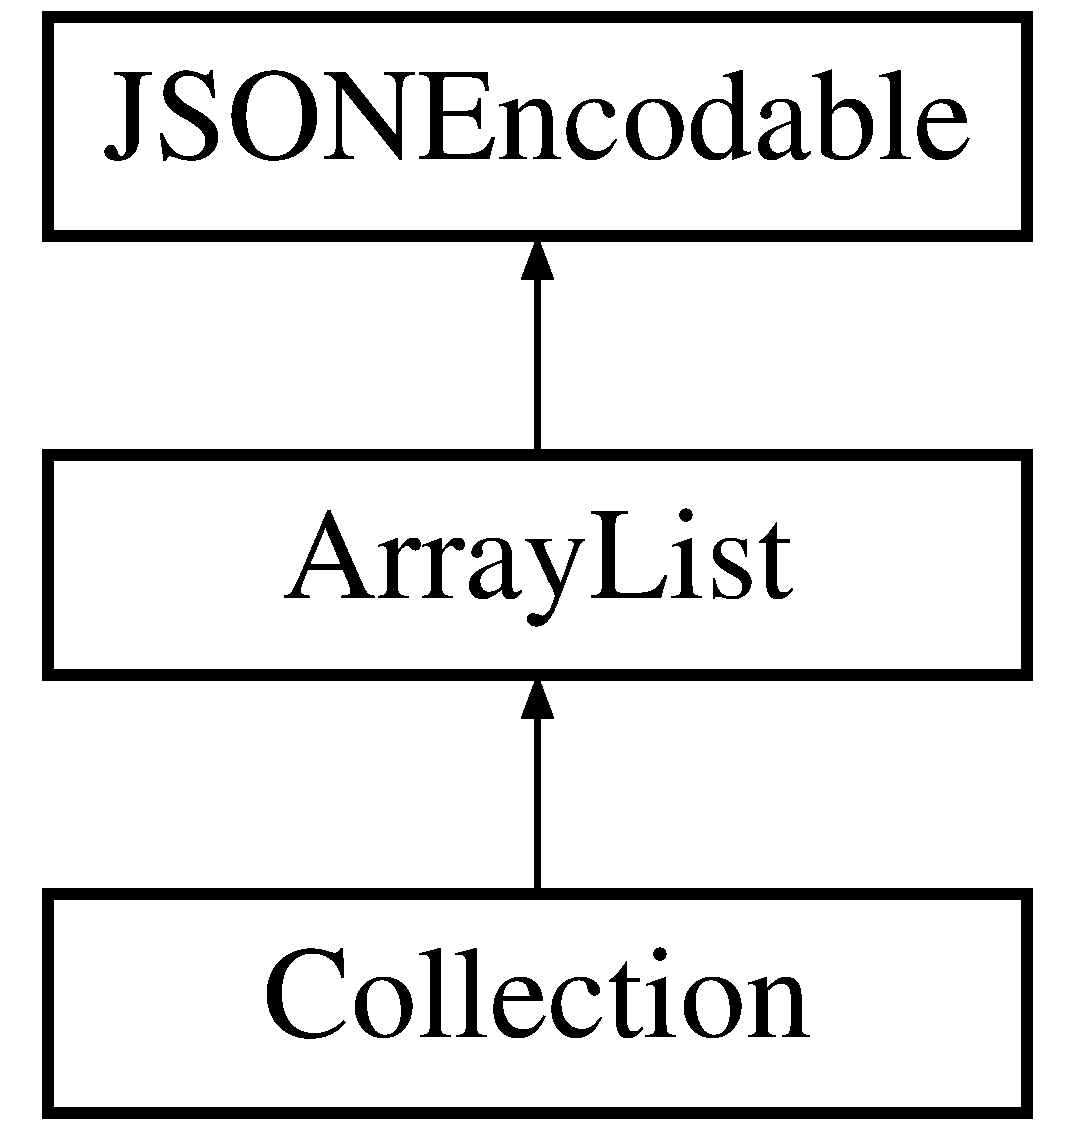
\includegraphics[height=4.000000cm]{classArrayList}
\end{center}
\end{figure}
\subsection*{Public Member Functions}
\begin{DoxyCompactItemize}
\item 
\hypertarget{classArrayList_a9d768c4cd89527c088c22f37682a3dd9}{
{\bfseries \_\-\_\-construct} (\$data=null)}
\label{classArrayList_a9d768c4cd89527c088c22f37682a3dd9}

\item 
\hyperlink{classArrayList_af3b2589a8217fd3940a2c5c02f013464}{implode} (\$glue)
\item 
\hypertarget{classArrayList_a431e2b6b4e80c2a394ed6650ca0cd704}{
{\bfseries explode} (\$glue)}
\label{classArrayList_a431e2b6b4e80c2a394ed6650ca0cd704}

\item 
\hypertarget{classArrayList_aab49ce13cee86e394f056cbb58a87c42}{
{\bfseries keys} ()}
\label{classArrayList_aab49ce13cee86e394f056cbb58a87c42}

\item 
\hyperlink{classArrayList_acfdc7b238672ea487ca21bd25725eef0}{merge} (\$other, \$overwrite=false)
\item 
\hypertarget{classArrayList_a0893e98494e2fa50e7e599e02702519e}{
{\bfseries usort} (\$callback)}
\label{classArrayList_a0893e98494e2fa50e7e599e02702519e}

\item 
\hyperlink{classArrayList_ad6b02815f556ca7a76494ed12b27aa96}{current} ()
\item 
\hypertarget{classArrayList_a87515f60ae4ebdd0539cfcadf2a5d0dc}{
{\bfseries rewind} ()}
\label{classArrayList_a87515f60ae4ebdd0539cfcadf2a5d0dc}

\item 
\hypertarget{classArrayList_ae2bb108208e1b5d29f93e0a7d8a21542}{
{\bfseries key} ()}
\label{classArrayList_ae2bb108208e1b5d29f93e0a7d8a21542}

\item 
\hypertarget{classArrayList_aa62b47db8550898b560734aca682d092}{
{\bfseries next} ()}
\label{classArrayList_aa62b47db8550898b560734aca682d092}

\item 
\hypertarget{classArrayList_a332cddf64ac35efc06c4c56593f38064}{
{\bfseries valid} ()}
\label{classArrayList_a332cddf64ac35efc06c4c56593f38064}

\item 
\hyperlink{classArrayList_a149d12c4042fe070f7579bce33eed2ce}{count} ()
\item 
\hyperlink{classArrayList_a18a60fa294bfba47839e27412f713ab6}{offsetExists} (\$offset)
\item 
\hypertarget{classArrayList_ae0353aa1d538eff8cfb70d0e41c3a1e5}{
{\bfseries offsetGet} (\$offset=null)}
\label{classArrayList_ae0353aa1d538eff8cfb70d0e41c3a1e5}

\item 
\hypertarget{classArrayList_a90473248c6f6b2fa58717cb2bedbc94e}{
{\bfseries offsetSet} (\$offset, \$value)}
\label{classArrayList_a90473248c6f6b2fa58717cb2bedbc94e}

\item 
\hypertarget{classArrayList_a32abe6ce9d3649778a3b146c953fad3b}{
{\bfseries offsetUnset} (\$offset)}
\label{classArrayList_a32abe6ce9d3649778a3b146c953fad3b}

\item 
\hyperlink{classArrayList_af8a43bf653ecd0dc477c89d525ca1695}{push} (\$item)
\item 
\hypertarget{classArrayList_ac1d51079cc61e1e94ad1766a1842a97f}{
{\bfseries pop} ()}
\label{classArrayList_ac1d51079cc61e1e94ad1766a1842a97f}

\item 
\hypertarget{classArrayList_a4d3b61218b90023d52486c6b3dbcf314}{
{\bfseries shift} ()}
\label{classArrayList_a4d3b61218b90023d52486c6b3dbcf314}

\item 
\hypertarget{classArrayList_a197cee959e624c083c4285754af05680}{
{\bfseries unshift} (\$item)}
\label{classArrayList_a197cee959e624c083c4285754af05680}

\item 
\hypertarget{classArrayList_ab98a7fb4149de5e31b39fe0bbe4d435e}{
{\bfseries get} (\$index=null)}
\label{classArrayList_ab98a7fb4149de5e31b39fe0bbe4d435e}

\item 
\hypertarget{classArrayList_a70cffc1017606dc401bacef19a4b2f42}{
{\bfseries set} (\$index, \$value)}
\label{classArrayList_a70cffc1017606dc401bacef19a4b2f42}

\item 
\hypertarget{classArrayList_a10020679f12e299af894de406eb4f34e}{
{\bfseries remove} (\$index)}
\label{classArrayList_a10020679f12e299af894de406eb4f34e}

\item 
\hypertarget{classArrayList_a04aef6ed21c038bf15e708a8dea8c7d1}{
{\bfseries reverse} ()}
\label{classArrayList_a04aef6ed21c038bf15e708a8dea8c7d1}

\end{DoxyCompactItemize}
\subsection*{Protected Attributes}
\begin{DoxyCompactItemize}
\item 
\hypertarget{classArrayList_aa2020764364f5af7bde0001145eb1e04}{
{\bfseries \$\_\-data} = array()}
\label{classArrayList_aa2020764364f5af7bde0001145eb1e04}

\end{DoxyCompactItemize}


\subsection{Detailed Description}
Handles all array-\/type structure that also require supplemental information or methods. This may get changed to simply extend ArrayObject 

\subsection{Member Function Documentation}
\hypertarget{classArrayList_a149d12c4042fe070f7579bce33eed2ce}{
\index{ArrayList@{ArrayList}!count@{count}}
\index{count@{count}!ArrayList@{ArrayList}}
\subsubsection[{count}]{\setlength{\rightskip}{0pt plus 5cm}ArrayList::count (
\begin{DoxyParamCaption}
{}
\end{DoxyParamCaption}
)}}
\label{classArrayList_a149d12c4042fe070f7579bce33eed2ce}
Countable method \hypertarget{classArrayList_ad6b02815f556ca7a76494ed12b27aa96}{
\index{ArrayList@{ArrayList}!current@{current}}
\index{current@{current}!ArrayList@{ArrayList}}
\subsubsection[{current}]{\setlength{\rightskip}{0pt plus 5cm}ArrayList::current (
\begin{DoxyParamCaption}
{}
\end{DoxyParamCaption}
)}}
\label{classArrayList_ad6b02815f556ca7a76494ed12b27aa96}
Iterator methods \hypertarget{classArrayList_af3b2589a8217fd3940a2c5c02f013464}{
\index{ArrayList@{ArrayList}!implode@{implode}}
\index{implode@{implode}!ArrayList@{ArrayList}}
\subsubsection[{implode}]{\setlength{\rightskip}{0pt plus 5cm}ArrayList::implode (
\begin{DoxyParamCaption}
\item[{\$}]{ glue}
\end{DoxyParamCaption}
)}}
\label{classArrayList_af3b2589a8217fd3940a2c5c02f013464}
Simulates implode/explode (requires all items to be castable as strings). \hypertarget{classArrayList_acfdc7b238672ea487ca21bd25725eef0}{
\index{ArrayList@{ArrayList}!merge@{merge}}
\index{merge@{merge}!ArrayList@{ArrayList}}
\subsubsection[{merge}]{\setlength{\rightskip}{0pt plus 5cm}ArrayList::merge (
\begin{DoxyParamCaption}
\item[{\$}]{ other, }
\item[{\$}]{ overwrite = {\ttfamily false}}
\end{DoxyParamCaption}
)}}
\label{classArrayList_acfdc7b238672ea487ca21bd25725eef0}
Merges another arraylist into this one \hypertarget{classArrayList_a18a60fa294bfba47839e27412f713ab6}{
\index{ArrayList@{ArrayList}!offsetExists@{offsetExists}}
\index{offsetExists@{offsetExists}!ArrayList@{ArrayList}}
\subsubsection[{offsetExists}]{\setlength{\rightskip}{0pt plus 5cm}ArrayList::offsetExists (
\begin{DoxyParamCaption}
\item[{\$}]{ offset}
\end{DoxyParamCaption}
)}}
\label{classArrayList_a18a60fa294bfba47839e27412f713ab6}
ArrayAccess methods \hypertarget{classArrayList_af8a43bf653ecd0dc477c89d525ca1695}{
\index{ArrayList@{ArrayList}!push@{push}}
\index{push@{push}!ArrayList@{ArrayList}}
\subsubsection[{push}]{\setlength{\rightskip}{0pt plus 5cm}ArrayList::push (
\begin{DoxyParamCaption}
\item[{\$}]{ item}
\end{DoxyParamCaption}
)}}
\label{classArrayList_af8a43bf653ecd0dc477c89d525ca1695}
Basic array methods 

Reimplemented in \hyperlink{classCollection_afa19de785c3fb54f187786782d082733}{Collection}.



The documentation for this class was generated from the following file:\begin{DoxyCompactItemize}
\item 
Library/ArrayList.php\end{DoxyCompactItemize}

\hypertarget{classCollection}{
\section{Collection Class Reference}
\label{classCollection}\index{Collection@{Collection}}
}
Inheritance diagram for Collection:\begin{figure}[H]
\begin{center}
\leavevmode
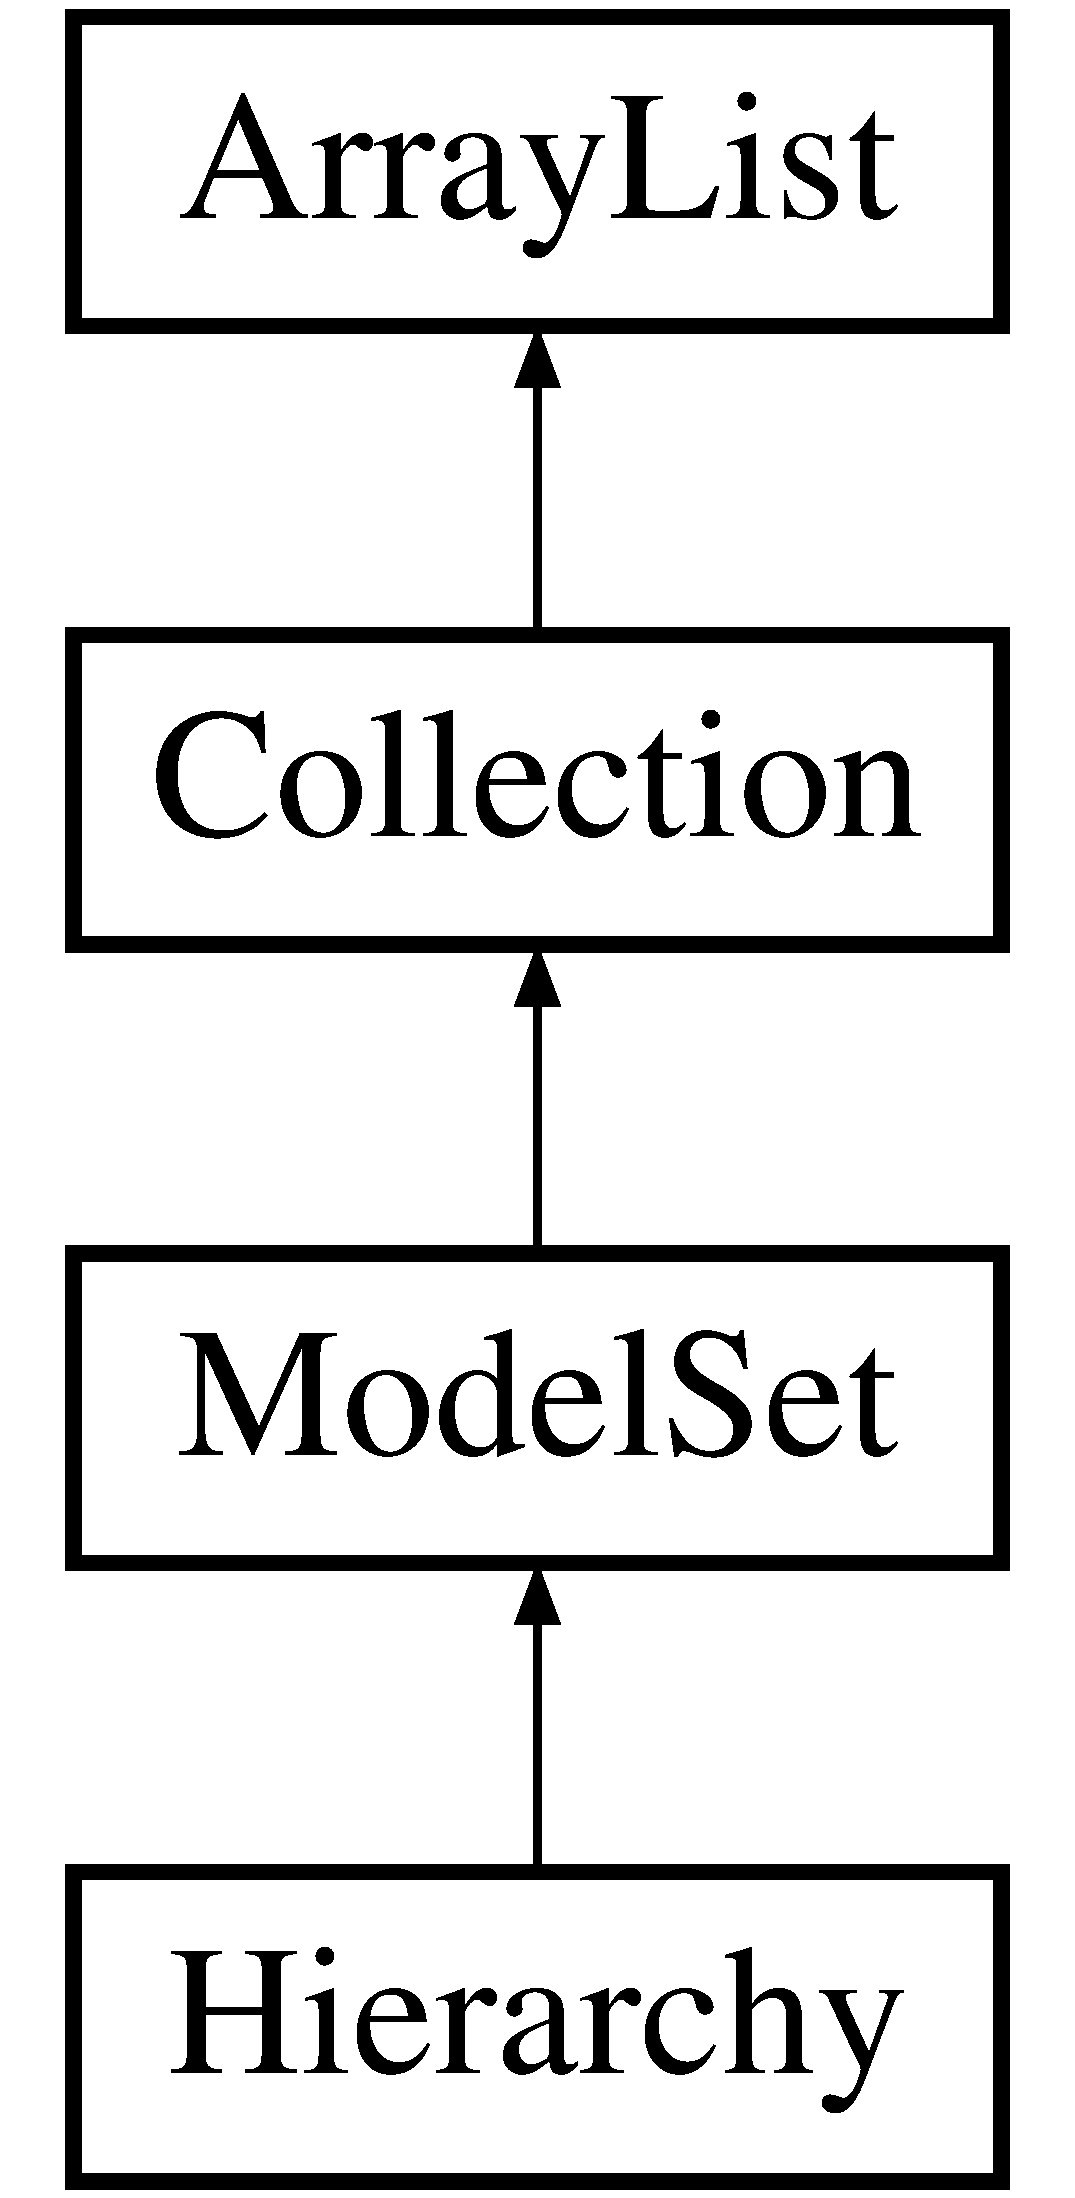
\includegraphics[height=4.000000cm]{classCollection}
\end{center}
\end{figure}
\subsection*{Public Member Functions}
\begin{DoxyCompactItemize}
\item 
\hypertarget{classCollection_a24944b0b4138f2d5ec0a1cbb9bc85ade}{
{\bfseries \_\-\_\-construct} (\$type, \$data=null)}
\label{classCollection_a24944b0b4138f2d5ec0a1cbb9bc85ade}

\item 
\hypertarget{classCollection_a1d8e8a80564ac93eb8d636e7877447ec}{
{\bfseries set} (\$index, \$value)}
\label{classCollection_a1d8e8a80564ac93eb8d636e7877447ec}

\item 
\hypertarget{classCollection_aebaa5b4f4f01e5bb8cd80a6b8d68358b}{
{\bfseries unshift} (\$item)}
\label{classCollection_aebaa5b4f4f01e5bb8cd80a6b8d68358b}

\item 
\hyperlink{classCollection_afa19de785c3fb54f187786782d082733}{push} (\$item)
\item 
\hypertarget{classCollection_ab889e651767d1598189ab61b4a3c75f8}{
{\bfseries welcomes} (\$item)}
\label{classCollection_ab889e651767d1598189ab61b4a3c75f8}

\item 
\hypertarget{classCollection_a3db7e9a0b39b65f39677b549364547f3}{
{\bfseries type} ()}
\label{classCollection_a3db7e9a0b39b65f39677b549364547f3}

\item 
\hyperlink{classCollection_a20622fcde06bbba3f05487f26773eef6}{\_\-\_\-get} (\$name)
\item 
\hyperlink{classCollection_a9e79c3f33f3780c717b06ba727484dcc}{\_\-\_\-set} (\$name, \$value)
\item 
\hyperlink{classCollection_aa4a0ddb57505aa399a273b061e997108}{\_\-\_\-call} (\$method, \$args)
\item 
\hyperlink{classCollection_a2ed1317fa00c1096a60a6877e1fa245f}{indexBy} (\$property)
\item 
\hyperlink{classCollection_a8d86dc7d75820b2646ee91f79317feec}{sortBy} (\$property, \$direction=ASC)
\end{DoxyCompactItemize}
\subsection*{Protected Attributes}
\begin{DoxyCompactItemize}
\item 
\hypertarget{classCollection_a4273177d393e56c83a13923c3bd6f499}{
{\bfseries \$\_\-type}}
\label{classCollection_a4273177d393e56c83a13923c3bd6f499}

\end{DoxyCompactItemize}


\subsection{Detailed Description}
Used for sets of objects that are intended to be iterated and counted like arrays, but allows storage of extra data that arrays do not. 

\subsection{Member Function Documentation}
\hypertarget{classCollection_aa4a0ddb57505aa399a273b061e997108}{
\index{Collection@{Collection}!\_\-\_\-call@{\_\-\_\-call}}
\index{\_\-\_\-call@{\_\-\_\-call}!Collection@{Collection}}
\subsubsection[{\_\-\_\-call}]{\setlength{\rightskip}{0pt plus 5cm}Collection::\_\-\_\-call (
\begin{DoxyParamCaption}
\item[{\$}]{ method, }
\item[{\$}]{ args}
\end{DoxyParamCaption}
)}}
\label{classCollection_aa4a0ddb57505aa399a273b061e997108}
Calling a method will return an array of the result of that method being called on all items in the collection. \hypertarget{classCollection_a20622fcde06bbba3f05487f26773eef6}{
\index{Collection@{Collection}!\_\-\_\-get@{\_\-\_\-get}}
\index{\_\-\_\-get@{\_\-\_\-get}!Collection@{Collection}}
\subsubsection[{\_\-\_\-get}]{\setlength{\rightskip}{0pt plus 5cm}Collection::\_\-\_\-get (
\begin{DoxyParamCaption}
\item[{\$}]{ name}
\end{DoxyParamCaption}
)}}
\label{classCollection_a20622fcde06bbba3f05487f26773eef6}
Getting a value from the collection will return an array of that value from each collection item. \hypertarget{classCollection_a9e79c3f33f3780c717b06ba727484dcc}{
\index{Collection@{Collection}!\_\-\_\-set@{\_\-\_\-set}}
\index{\_\-\_\-set@{\_\-\_\-set}!Collection@{Collection}}
\subsubsection[{\_\-\_\-set}]{\setlength{\rightskip}{0pt plus 5cm}Collection::\_\-\_\-set (
\begin{DoxyParamCaption}
\item[{\$}]{ name, }
\item[{\$}]{ value}
\end{DoxyParamCaption}
)}}
\label{classCollection_a9e79c3f33f3780c717b06ba727484dcc}
Setting a value to the collection will attempt to set that value in all collection items. \hypertarget{classCollection_a2ed1317fa00c1096a60a6877e1fa245f}{
\index{Collection@{Collection}!indexBy@{indexBy}}
\index{indexBy@{indexBy}!Collection@{Collection}}
\subsubsection[{indexBy}]{\setlength{\rightskip}{0pt plus 5cm}Collection::indexBy (
\begin{DoxyParamCaption}
\item[{\$}]{ property}
\end{DoxyParamCaption}
)}}
\label{classCollection_a2ed1317fa00c1096a60a6877e1fa245f}
Indexes the objects by the specified property. \hypertarget{classCollection_afa19de785c3fb54f187786782d082733}{
\index{Collection@{Collection}!push@{push}}
\index{push@{push}!Collection@{Collection}}
\subsubsection[{push}]{\setlength{\rightskip}{0pt plus 5cm}Collection::push (
\begin{DoxyParamCaption}
\item[{\$}]{ item}
\end{DoxyParamCaption}
)}}
\label{classCollection_afa19de785c3fb54f187786782d082733}
Basic array methods 

Reimplemented from \hyperlink{classArrayList_af8a43bf653ecd0dc477c89d525ca1695}{ArrayList}.

\hypertarget{classCollection_a8d86dc7d75820b2646ee91f79317feec}{
\index{Collection@{Collection}!sortBy@{sortBy}}
\index{sortBy@{sortBy}!Collection@{Collection}}
\subsubsection[{sortBy}]{\setlength{\rightskip}{0pt plus 5cm}Collection::sortBy (
\begin{DoxyParamCaption}
\item[{\$}]{ property, }
\item[{\$}]{ direction = {\ttfamily ASC}}
\end{DoxyParamCaption}
)}}
\label{classCollection_a8d86dc7d75820b2646ee91f79317feec}
Sorts objects in the collection by the specified property. 

The documentation for this class was generated from the following file:\begin{DoxyCompactItemize}
\item 
Library/Collection.php\end{DoxyCompactItemize}

\hypertarget{classComponent}{
\section{Component Class Reference}
\label{classComponent}\index{Component@{Component}}
}
Inheritance diagram for Component:\begin{figure}[H]
\begin{center}
\leavevmode
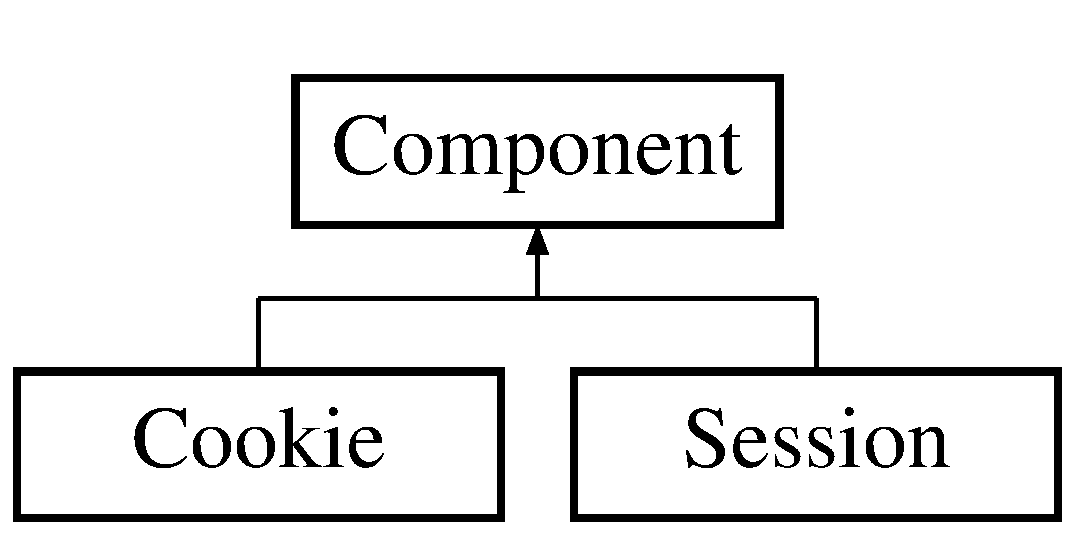
\includegraphics[height=2.000000cm]{classComponent}
\end{center}
\end{figure}
\subsection*{Public Member Functions}
\begin{DoxyCompactItemize}
\item 
\hypertarget{classComponent_aaa6259b967067c4616a8b33a92bbb616}{
{\bfseries \_\-\_\-construct} (\$controller)}
\label{classComponent_aaa6259b967067c4616a8b33a92bbb616}

\item 
\hypertarget{classComponent_ae72a2aff44cb477971a8649abba407cd}{
{\bfseries \_\-\_\-get} (\$name)}
\label{classComponent_ae72a2aff44cb477971a8649abba407cd}

\end{DoxyCompactItemize}
\subsection*{Protected Member Functions}
\begin{DoxyCompactItemize}
\item 
\hypertarget{classComponent_ae69207eea0ccf6cc855e74fa05b6db17}{
{\bfseries \_\-init} ()}
\label{classComponent_ae69207eea0ccf6cc855e74fa05b6db17}

\end{DoxyCompactItemize}
\subsection*{Protected Attributes}
\begin{DoxyCompactItemize}
\item 
\hypertarget{classComponent_a560d57b5dbdc6a452d39efd2a8effc49}{
{\bfseries \$\_\-Controller}}
\label{classComponent_a560d57b5dbdc6a452d39efd2a8effc49}

\end{DoxyCompactItemize}


\subsection{Detailed Description}
Base \hyperlink{classComponent}{Component} class for the \hyperlink{classFrawst}{Frawst} framework.

Components are modular extensions of controller (business) logic. 

The documentation for this class was generated from the following file:\begin{DoxyCompactItemize}
\item 
Component.php\end{DoxyCompactItemize}

\hypertarget{classConfig}{
\section{Config Class Reference}
\label{classConfig}\index{Config@{Config}}
}
\subsection*{Static Public Member Functions}
\begin{DoxyCompactItemize}
\item 
\hypertarget{classConfig_a25bd8da6939a4173a5eb6b55281c02da}{
static {\bfseries read} (\$dotPath)}
\label{classConfig_a25bd8da6939a4173a5eb6b55281c02da}

\end{DoxyCompactItemize}
\subsection*{Static Protected Attributes}
\begin{DoxyCompactItemize}
\item 
\hypertarget{classConfig_aec55d9da7c6ae27a0568e01b0060b9ed}{
static {\bfseries \$\_\-data} = array()}
\label{classConfig_aec55d9da7c6ae27a0568e01b0060b9ed}

\end{DoxyCompactItemize}


\subsection{Detailed Description}
\hyperlink{classConfig}{Config}

Reads variables from configuration files. \begin{Desc}
\item[\hyperlink{todo__todo000001}{Todo}]Make this instantiable \end{Desc}


The documentation for this class was generated from the following file:\begin{DoxyCompactItemize}
\item 
libs/Config.php\end{DoxyCompactItemize}

\hypertarget{classController}{
\section{Controller Class Reference}
\label{classController}\index{Controller@{Controller}}
}
Inheritance diagram for Controller:\begin{figure}[H]
\begin{center}
\leavevmode
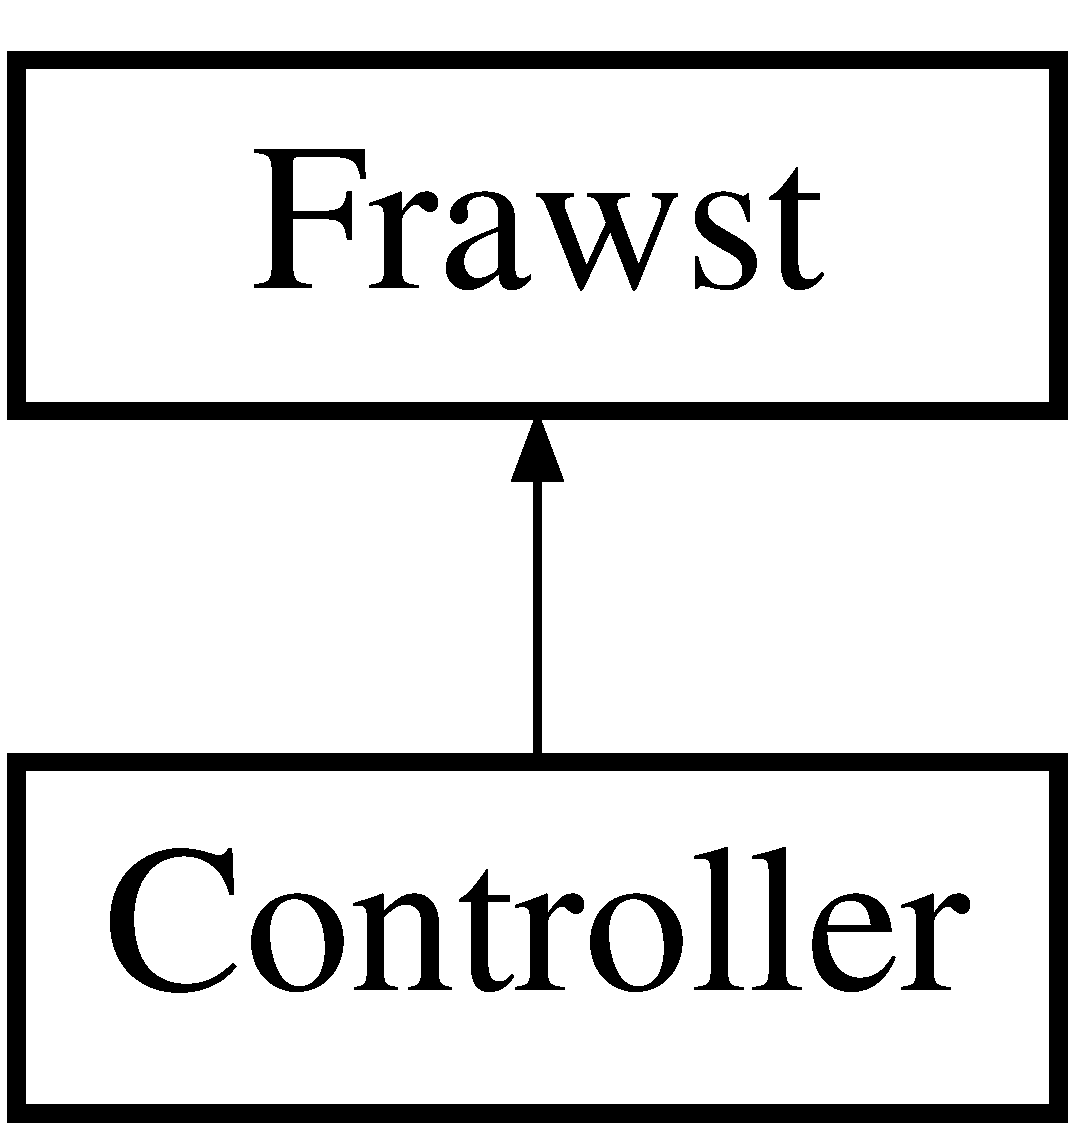
\includegraphics[height=2.000000cm]{classController}
\end{center}
\end{figure}
\subsection*{Public Member Functions}
\begin{DoxyCompactItemize}
\item 
\hyperlink{classController_ab91faf91a99b21a429324499f9ec9f70}{\_\-\_\-construct} (\$request)
\item 
\hyperlink{classController_ae031bdcdd680eafcc1f36f497db0cdcf}{\_\-\_\-get} (\$name)
\item 
\hyperlink{classController_a9f80ff7e29e17e2de1da86a2ccf4141e}{execute} ()
\end{DoxyCompactItemize}
\subsection*{Protected Member Functions}
\begin{DoxyCompactItemize}
\item 
\hyperlink{classController_ad39427afb53b12d4fc3b037cdd7d01b6}{\_\-before} ()
\item 
\hyperlink{classController_a7f25281d53ef0fed70ae0d687d2cea99}{\_\-after} (\$data)
\item 
\hyperlink{classController_ac425af9dbdb9979417c81a7c07ca6c28}{\_\-component} (\$name)
\end{DoxyCompactItemize}
\subsection*{Protected Attributes}
\begin{DoxyCompactItemize}
\item 
\hypertarget{classController_a9d857b6c224db9e835893cbb77b72028}{
{\bfseries \$\_\-components}}
\label{classController_a9d857b6c224db9e835893cbb77b72028}

\item 
\hypertarget{classController_a00a97dc8ec158668a2689614ee3ecd2b}{
{\bfseries \$\_\-data}}
\label{classController_a00a97dc8ec158668a2689614ee3ecd2b}

\item 
\hypertarget{classController_ad913df9bc5d91dcd80c26bc5e316e726}{
{\bfseries \$\_\-Request}}
\label{classController_ad913df9bc5d91dcd80c26bc5e316e726}

\end{DoxyCompactItemize}


\subsection{Detailed Description}
Base \hyperlink{classController}{Controller} class for the \hyperlink{classFrawst}{Frawst} framework. 

\subsection{Constructor \& Destructor Documentation}
\hypertarget{classController_ab91faf91a99b21a429324499f9ec9f70}{
\index{Controller@{Controller}!\_\-\_\-construct@{\_\-\_\-construct}}
\index{\_\-\_\-construct@{\_\-\_\-construct}!Controller@{Controller}}
\subsubsection[{\_\-\_\-construct}]{\setlength{\rightskip}{0pt plus 5cm}Controller::\_\-\_\-construct (
\begin{DoxyParamCaption}
\item[{\$}]{ request}
\end{DoxyParamCaption}
)}}
\label{classController_ab91faf91a99b21a429324499f9ec9f70}
Constructor. 
\begin{DoxyParams}{Parameters}
\item[{\em Frawst$\backslash$Request}]The request using the controller \end{DoxyParams}


\subsection{Member Function Documentation}
\hypertarget{classController_ae031bdcdd680eafcc1f36f497db0cdcf}{
\index{Controller@{Controller}!\_\-\_\-get@{\_\-\_\-get}}
\index{\_\-\_\-get@{\_\-\_\-get}!Controller@{Controller}}
\subsubsection[{\_\-\_\-get}]{\setlength{\rightskip}{0pt plus 5cm}Controller::\_\-\_\-get (
\begin{DoxyParamCaption}
\item[{\$}]{ name}
\end{DoxyParamCaption}
)}}
\label{classController_ae031bdcdd680eafcc1f36f497db0cdcf}
Read-\/only immitation. 
\begin{DoxyParams}{Parameters}
\item[{\em string}]\$name \end{DoxyParams}
\begin{DoxyReturn}{Returns}
mixed 
\end{DoxyReturn}
\hypertarget{classController_a7f25281d53ef0fed70ae0d687d2cea99}{
\index{Controller@{Controller}!\_\-after@{\_\-after}}
\index{\_\-after@{\_\-after}!Controller@{Controller}}
\subsubsection[{\_\-after}]{\setlength{\rightskip}{0pt plus 5cm}Controller::\_\-after (
\begin{DoxyParamCaption}
\item[{\$}]{ data}
\end{DoxyParamCaption}
)\hspace{0.3cm}{\ttfamily  \mbox{[}protected\mbox{]}}}}
\label{classController_a7f25281d53ef0fed70ae0d687d2cea99}
Invoked after execution. 
\begin{DoxyParams}{Parameters}
\item[{\em mixed}]\$data The value returned from execution \end{DoxyParams}
\begin{DoxyReturn}{Returns}
mixed The data that should be stored in the \hyperlink{classResponse}{Response} 
\end{DoxyReturn}
\hypertarget{classController_ad39427afb53b12d4fc3b037cdd7d01b6}{
\index{Controller@{Controller}!\_\-before@{\_\-before}}
\index{\_\-before@{\_\-before}!Controller@{Controller}}
\subsubsection[{\_\-before}]{\setlength{\rightskip}{0pt plus 5cm}Controller::\_\-before (
\begin{DoxyParamCaption}
{}
\end{DoxyParamCaption}
)\hspace{0.3cm}{\ttfamily  \mbox{[}protected\mbox{]}}}}
\label{classController_ad39427afb53b12d4fc3b037cdd7d01b6}
Invoked before execution. \begin{DoxyReturn}{Returns}
bool false if execution should not proceed, true otherwise 
\end{DoxyReturn}
\hypertarget{classController_ac425af9dbdb9979417c81a7c07ca6c28}{
\index{Controller@{Controller}!\_\-component@{\_\-component}}
\index{\_\-component@{\_\-component}!Controller@{Controller}}
\subsubsection[{\_\-component}]{\setlength{\rightskip}{0pt plus 5cm}Controller::\_\-component (
\begin{DoxyParamCaption}
\item[{\$}]{ name}
\end{DoxyParamCaption}
)\hspace{0.3cm}{\ttfamily  \mbox{[}protected\mbox{]}}}}
\label{classController_ac425af9dbdb9979417c81a7c07ca6c28}
Attempts to access a component. If the component class exists but has not yet been instantiated for this controller, instantiation will happen first. 
\begin{DoxyParams}{Parameters}
\item[{\em string}]\$name Name of the component \end{DoxyParams}
\begin{DoxyReturn}{Returns}
mixed The component object, or false if the component does not exist 
\end{DoxyReturn}
\hypertarget{classController_a9f80ff7e29e17e2de1da86a2ccf4141e}{
\index{Controller@{Controller}!execute@{execute}}
\index{execute@{execute}!Controller@{Controller}}
\subsubsection[{execute}]{\setlength{\rightskip}{0pt plus 5cm}Controller::execute (
\begin{DoxyParamCaption}
{}
\end{DoxyParamCaption}
)}}
\label{classController_a9f80ff7e29e17e2de1da86a2ccf4141e}
Executes the controller logic. \hyperlink{classController_ad39427afb53b12d4fc3b037cdd7d01b6}{\_\-before()} and \hyperlink{classController_a7f25281d53ef0fed70ae0d687d2cea99}{\_\-after()} are invoked before and after the method logic. \begin{DoxyReturn}{Returns}
mixed The data to be sent in the \hyperlink{classResponse}{Response} 
\end{DoxyReturn}


The documentation for this class was generated from the following file:\begin{DoxyCompactItemize}
\item 
libs/Controller.php\end{DoxyCompactItemize}

\hypertarget{classCookie}{
\section{Cookie Class Reference}
\label{classCookie}\index{Cookie@{Cookie}}
}
Inheritance diagram for Cookie:\begin{figure}[H]
\begin{center}
\leavevmode
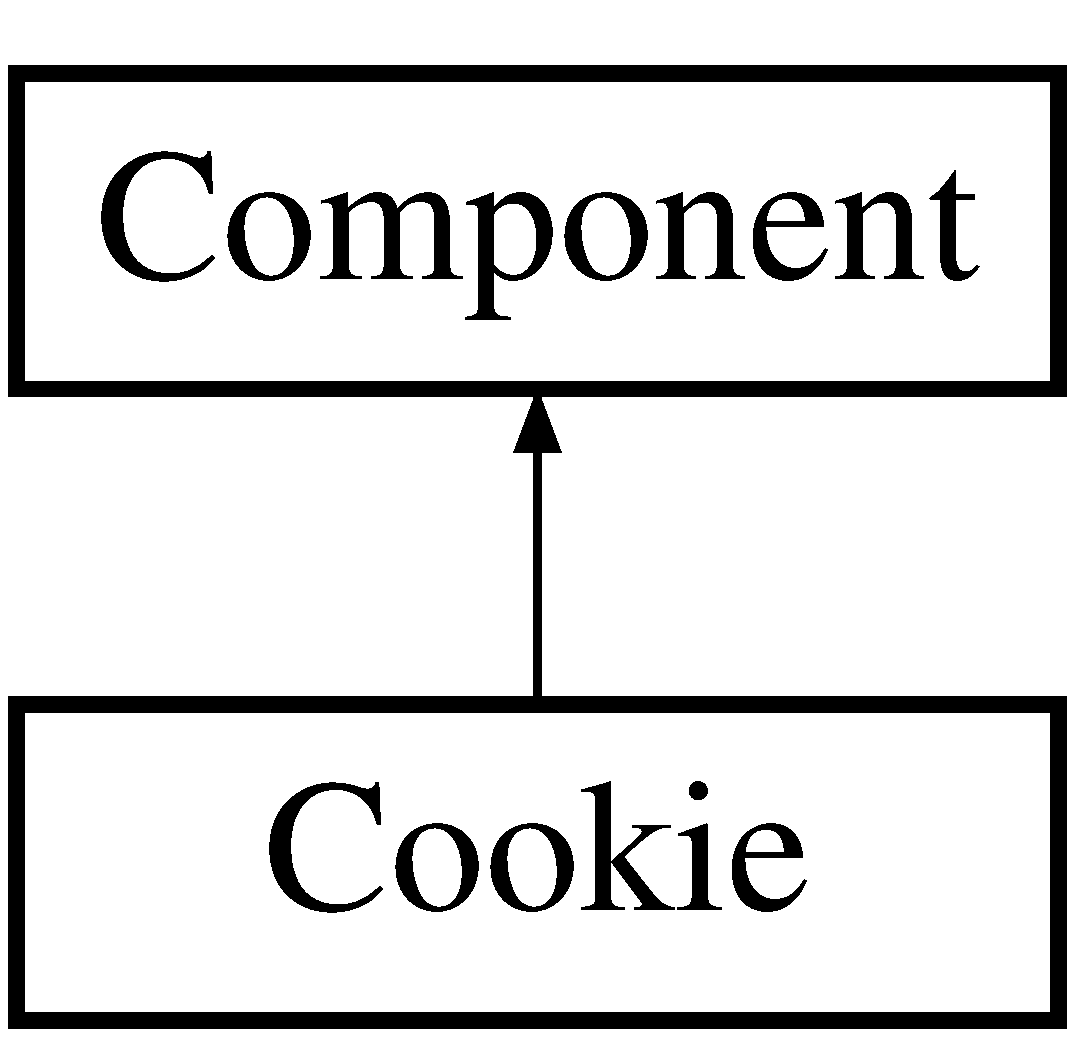
\includegraphics[height=2.000000cm]{classCookie}
\end{center}
\end{figure}
\subsection*{Public Member Functions}
\begin{DoxyCompactItemize}
\item 
\hypertarget{classCookie_a2d6eea6280981d7ab703772681f7a4aa}{
{\bfseries offsetSet} (\$offset, \$value)}
\label{classCookie_a2d6eea6280981d7ab703772681f7a4aa}

\item 
\hypertarget{classCookie_a17b6835c4e468e34741bd9ad4fa87fb5}{
{\bfseries offsetGet} (\$offset)}
\label{classCookie_a17b6835c4e468e34741bd9ad4fa87fb5}

\item 
\hypertarget{classCookie_aa473c0ae3cb07717be9b5b00aa59fe29}{
{\bfseries offsetExists} (\$offset)}
\label{classCookie_aa473c0ae3cb07717be9b5b00aa59fe29}

\item 
\hypertarget{classCookie_a076e18a6028d8cd5843060893e04e041}{
{\bfseries offsetUnset} (\$offset)}
\label{classCookie_a076e18a6028d8cd5843060893e04e041}

\item 
\hypertarget{classCookie_a2828d63c15838b350737e2be73be3ffa}{
{\bfseries \_\-\_\-construct} (\$name, \$value=null, \$expires=0, \$path=null, \$domain=null)}
\label{classCookie_a2828d63c15838b350737e2be73be3ffa}

\item 
\hypertarget{classCookie_a60f4d95767941d94c6fd06127f78af46}{
{\bfseries save} ()}
\label{classCookie_a60f4d95767941d94c6fd06127f78af46}

\item 
\hypertarget{classCookie_aaee9cc15f98661c022dc2728b48fa3a2}{
{\bfseries delete} ()}
\label{classCookie_aaee9cc15f98661c022dc2728b48fa3a2}

\end{DoxyCompactItemize}
\subsection*{Static Public Member Functions}
\begin{DoxyCompactItemize}
\item 
\hypertarget{classCookie_ad51a1a42a8cb4a60611e6dd1791478ac}{
static {\bfseries exists} (\$name)}
\label{classCookie_ad51a1a42a8cb4a60611e6dd1791478ac}

\end{DoxyCompactItemize}
\subsection*{Public Attributes}
\begin{DoxyCompactItemize}
\item 
\hypertarget{classCookie_ae670193bf994ae5869b31882154998d1}{
{\bfseries \$value}}
\label{classCookie_ae670193bf994ae5869b31882154998d1}

\item 
\hypertarget{classCookie_aefef959e4ccc496f73b90bafeabb7af2}{
{\bfseries \$expires}}
\label{classCookie_aefef959e4ccc496f73b90bafeabb7af2}

\item 
\hypertarget{classCookie_a25796543a5b84e9f81fd8ea355508d56}{
{\bfseries \$path}}
\label{classCookie_a25796543a5b84e9f81fd8ea355508d56}

\item 
\hypertarget{classCookie_a088cc3627624838d2eae7e72745a719b}{
{\bfseries \$domain}}
\label{classCookie_a088cc3627624838d2eae7e72745a719b}

\end{DoxyCompactItemize}
\subsection*{Protected Attributes}
\begin{DoxyCompactItemize}
\item 
\hypertarget{classCookie_add20beb35f6402602ba572988f4266aa}{
{\bfseries \$\_\-name}}
\label{classCookie_add20beb35f6402602ba572988f4266aa}

\end{DoxyCompactItemize}


The documentation for this class was generated from the following files:\begin{DoxyCompactItemize}
\item 
Component/Cookie.php\item 
Library/Cookie.php\end{DoxyCompactItemize}

\hypertarget{classData}{
\section{Data Class Reference}
\label{classData}\index{Data@{Data}}
}
Inheritance diagram for Data:\begin{figure}[H]
\begin{center}
\leavevmode
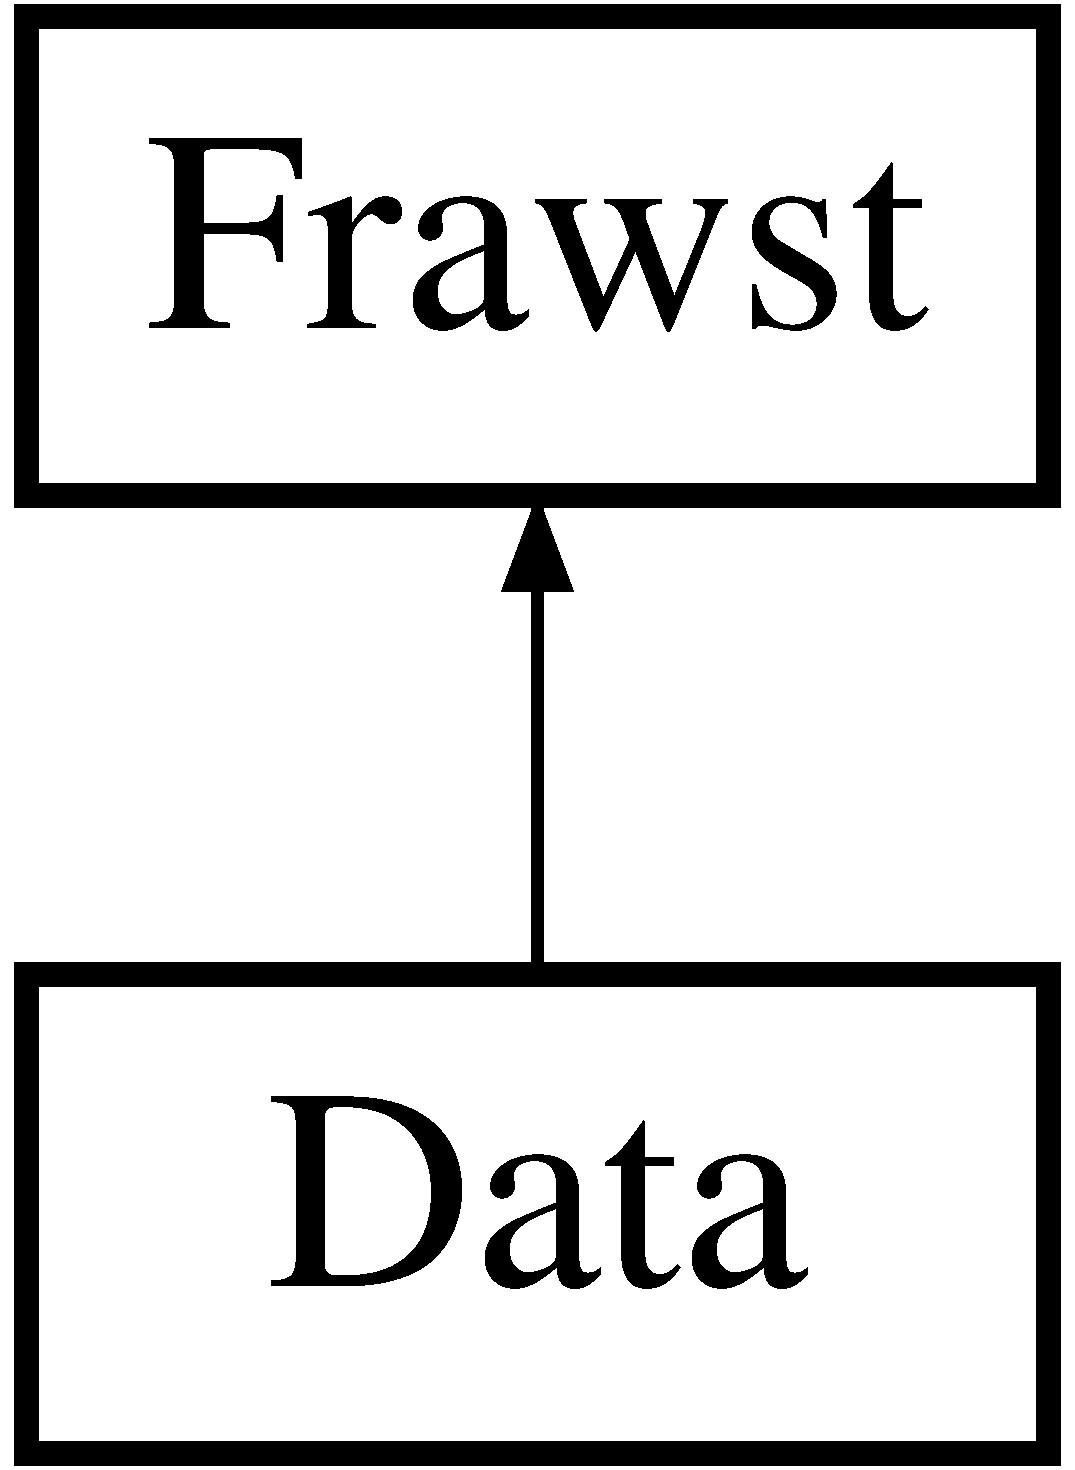
\includegraphics[height=2.000000cm]{classData}
\end{center}
\end{figure}


The documentation for this class was generated from the following file:\begin{DoxyCompactItemize}
\item 
libs/Exception/Data.php\end{DoxyCompactItemize}

\hypertarget{classDate}{
\section{Date Class Reference}
\label{classDate}\index{Date@{Date}}
}
\subsection*{Static Public Member Functions}
\begin{DoxyCompactItemize}
\item 
static \hyperlink{classDate_a9411511f91e820a9ffdedcbb4142fe32}{nice} (\$date, \$format= 'F j, Y')
\item 
static \hyperlink{classDate_a8a7c5375c96e43188434646202e71b07}{niceSpan} (\$seconds, \$precision=self::SECOND, \$cutoff=self::DAY, \$formats=array(), \$glue= ' ')
\end{DoxyCompactItemize}
\subsection*{Public Attributes}
\begin{DoxyCompactItemize}
\item 
\hypertarget{classDate_a8dfc17740f9b7a2f64a591a96f8a42fb}{
const {\bfseries SECOND} = 1}
\label{classDate_a8dfc17740f9b7a2f64a591a96f8a42fb}

\item 
\hypertarget{classDate_a7310a231d6b0235fc79589c878ca52c5}{
const {\bfseries MINUTE} = 60}
\label{classDate_a7310a231d6b0235fc79589c878ca52c5}

\item 
\hypertarget{classDate_aebd8725238ea4fab8803a489d083c66d}{
const {\bfseries HOUR} = 3600}
\label{classDate_aebd8725238ea4fab8803a489d083c66d}

\item 
\hypertarget{classDate_a1c78484633ffc685a1677c6b1185d5be}{
const {\bfseries DAY} = 86400}
\label{classDate_a1c78484633ffc685a1677c6b1185d5be}

\item 
\hypertarget{classDate_a834af4f51ff32608945ff6b571b57d06}{
const {\bfseries MONTH} = 2629744}
\label{classDate_a834af4f51ff32608945ff6b571b57d06}

\item 
\hypertarget{classDate_a88ff2c34643450905f490de48c0e4737}{
const {\bfseries YEAR} = 31556926}
\label{classDate_a88ff2c34643450905f490de48c0e4737}

\end{DoxyCompactItemize}


\subsection{Member Function Documentation}
\hypertarget{classDate_a9411511f91e820a9ffdedcbb4142fe32}{
\index{Date@{Date}!nice@{nice}}
\index{nice@{nice}!Date@{Date}}
\subsubsection[{nice}]{\setlength{\rightskip}{0pt plus 5cm}static Date::nice (
\begin{DoxyParamCaption}
\item[{\$}]{ date, }
\item[{\$}]{ format = {\ttfamily 'F~j}, }
\item[{Y'}]{}
\end{DoxyParamCaption}
)\hspace{0.3cm}{\ttfamily  \mbox{[}static\mbox{]}}}}
\label{classDate_a9411511f91e820a9ffdedcbb4142fe32}
Returns Today if the specified time falls during the current day, otherwise formats as specified. \hypertarget{classDate_a8a7c5375c96e43188434646202e71b07}{
\index{Date@{Date}!niceSpan@{niceSpan}}
\index{niceSpan@{niceSpan}!Date@{Date}}
\subsubsection[{niceSpan}]{\setlength{\rightskip}{0pt plus 5cm}static Date::niceSpan (
\begin{DoxyParamCaption}
\item[{\$}]{ seconds, }
\item[{\$}]{ precision = {\ttfamily self::SECOND}, }
\item[{\$}]{ cutoff = {\ttfamily self::DAY}, }
\item[{\$}]{ formats = {\ttfamily array()}, }
\item[{\$}]{ glue = {\ttfamily '~'}}
\end{DoxyParamCaption}
)\hspace{0.3cm}{\ttfamily  \mbox{[}static\mbox{]}}}}
\label{classDate_a8a7c5375c96e43188434646202e71b07}
Formats a time span.


\begin{DoxyParams}{Parameters}
\item[{\em seconds}]The number of seconds in the time span \item[{\em precision}]Smallest unit included \item[{\em cutoff}]If the span is $>$= this, only a single unit will be represented \item[{\em formats}]Formattings of each part \end{DoxyParams}


The documentation for this class was generated from the following file:\begin{DoxyCompactItemize}
\item 
Library/Date.php\end{DoxyCompactItemize}

\hypertarget{classFile}{
\section{File Class Reference}
\label{classFile}\index{File@{File}}
}
Inheritance diagram for File:\begin{figure}[H]
\begin{center}
\leavevmode
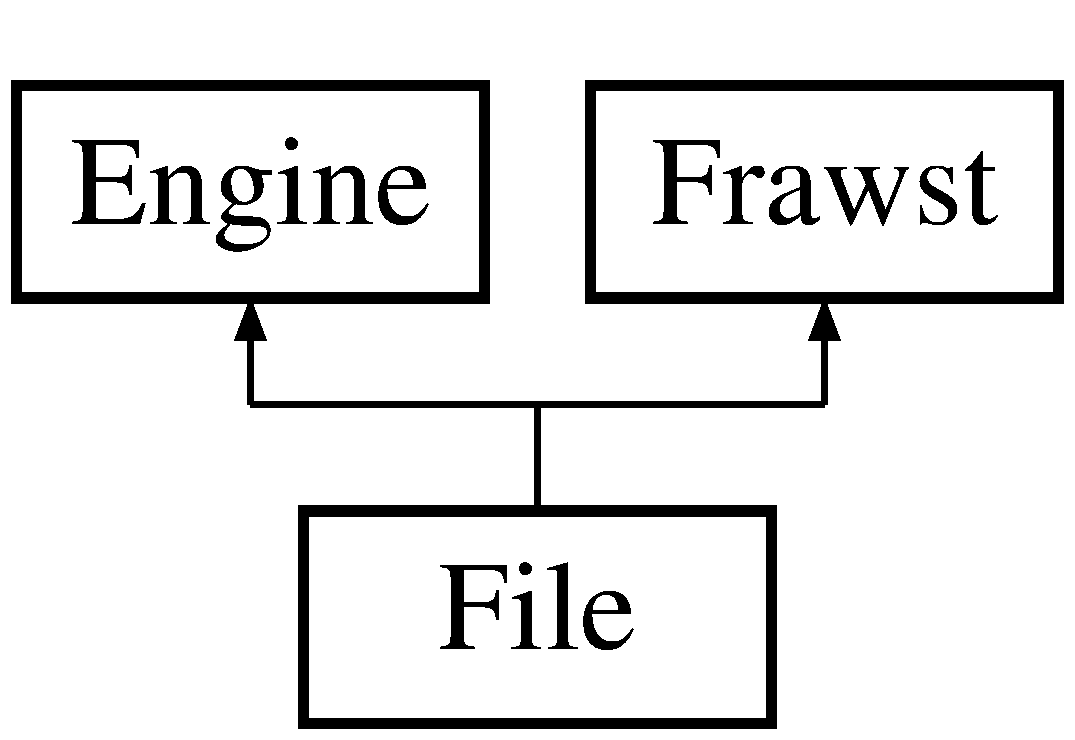
\includegraphics[height=2.000000cm]{classFile}
\end{center}
\end{figure}
\subsection*{Public Member Functions}
\begin{DoxyCompactItemize}
\item 
\hypertarget{classFile_a3c5141c5b72735f659cce3064b3a1218}{
{\bfseries \_\-\_\-construct} (\$config)}
\label{classFile_a3c5141c5b72735f659cce3064b3a1218}

\item 
\hypertarget{classFile_a8602a61364522be0f302e5a575a463db}{
{\bfseries expires} (\$name, \$time=null)}
\label{classFile_a8602a61364522be0f302e5a575a463db}

\item 
\hypertarget{classFile_a8253df2fba95c58851bc17e4f2dfd8d9}{
{\bfseries get} (\$name)}
\label{classFile_a8253df2fba95c58851bc17e4f2dfd8d9}

\item 
\hypertarget{classFile_a0f2b2116dd84ea00f15b86fa092263dd}{
{\bfseries exists} (\$name)}
\label{classFile_a0f2b2116dd84ea00f15b86fa092263dd}

\item 
\hypertarget{classFile_ada4df03846cee49c65296f7bd518bd3b}{
{\bfseries set} (\$name, \$value, \$life=0)}
\label{classFile_ada4df03846cee49c65296f7bd518bd3b}

\item 
\hypertarget{classFile_a9ec653c0f732bf4af8405b0ce82a040b}{
{\bfseries expire} (\$name)}
\label{classFile_a9ec653c0f732bf4af8405b0ce82a040b}

\end{DoxyCompactItemize}
\subsection*{Protected Attributes}
\begin{DoxyCompactItemize}
\item 
\hypertarget{classFile_ae3df9c154752d7a5892b5529cd58a59f}{
{\bfseries \$\_\-directory}}
\label{classFile_ae3df9c154752d7a5892b5529cd58a59f}

\item 
\hypertarget{classFile_a51d172324315d4db733bee91ee2f6109}{
{\bfseries \$\_\-data}}
\label{classFile_a51d172324315d4db733bee91ee2f6109}

\item 
\hypertarget{classFile_a947907f0953f4d5a88b8df5bf7402aa2}{
{\bfseries \$\_\-expire}}
\label{classFile_a947907f0953f4d5a88b8df5bf7402aa2}

\end{DoxyCompactItemize}


The documentation for this class was generated from the following files:\begin{DoxyCompactItemize}
\item 
Exception/File.php\item 
vendor/SimpleCache/Engine/File.php\end{DoxyCompactItemize}

\hypertarget{classFileMatrix}{
\section{FileMatrix Class Reference}
\label{classFileMatrix}\index{FileMatrix@{FileMatrix}}
}
Inheritance diagram for FileMatrix:\begin{figure}[H]
\begin{center}
\leavevmode
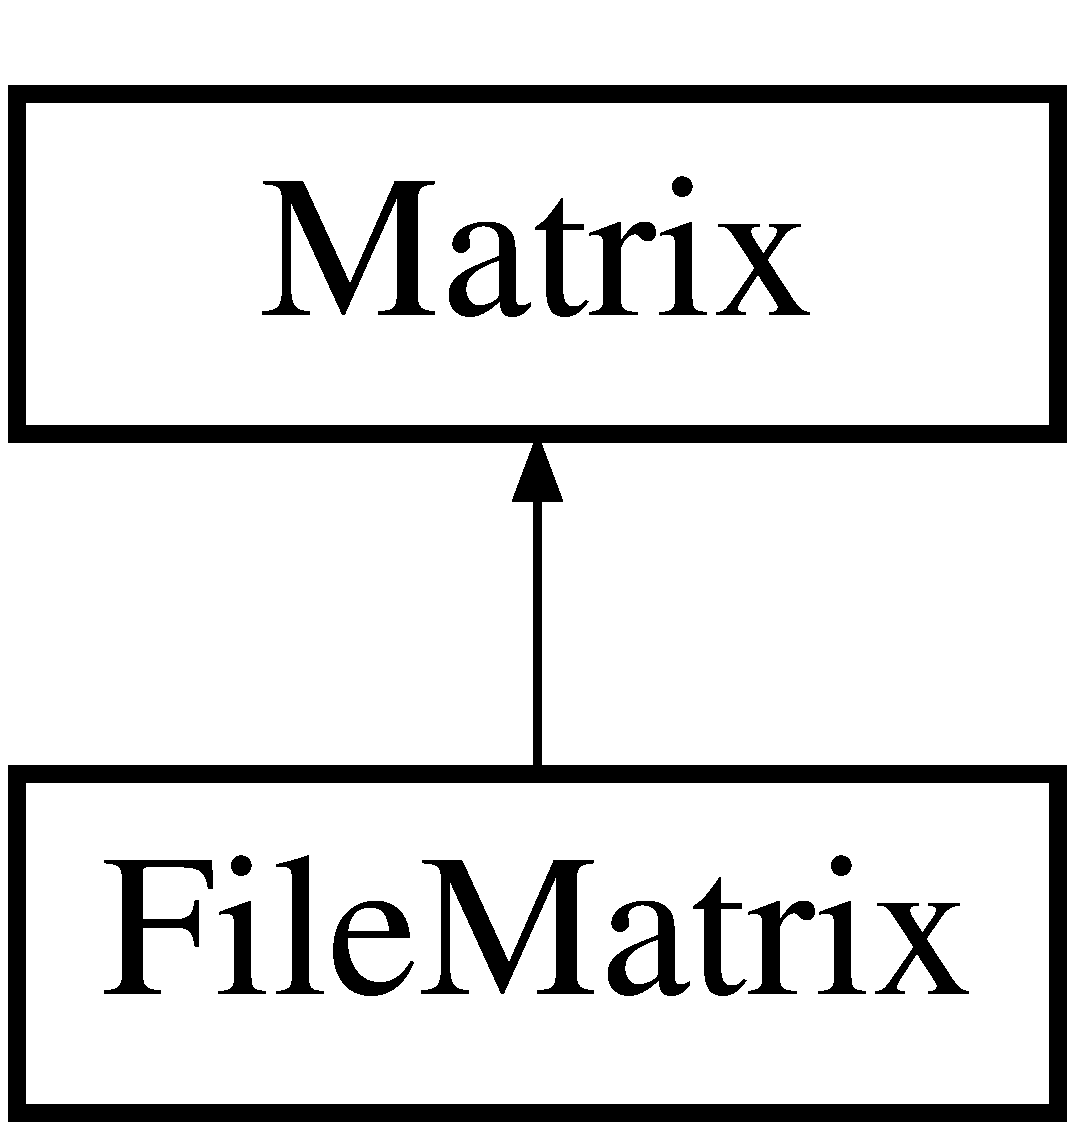
\includegraphics[height=2.000000cm]{classFileMatrix}
\end{center}
\end{figure}
\subsection*{Public Member Functions}
\begin{DoxyCompactItemize}
\item 
\hypertarget{classFileMatrix_a8fd49d801cf3714544267142030e0dec}{
{\bfseries \_\-\_\-construct} (\$directory, \$data=array())}
\label{classFileMatrix_a8fd49d801cf3714544267142030e0dec}

\item 
\hypertarget{classFileMatrix_aa553b9db2a4c33df0b034a86f04edaf6}{
{\bfseries offsetExists} (\$offset)}
\label{classFileMatrix_aa553b9db2a4c33df0b034a86f04edaf6}

\item 
\hyperlink{classFileMatrix_a0bd0b2818c4319b502c494d638525921}{offsetGet} (\$offset)
\item 
\hypertarget{classFileMatrix_a9e986f6aaa0e0871b5a0528025d6ccb9}{
{\bfseries offsetSet} (\$offset, \$value)}
\label{classFileMatrix_a9e986f6aaa0e0871b5a0528025d6ccb9}

\item 
\hypertarget{classFileMatrix_ac6479825abc7263f875afaf168740e98}{
{\bfseries offsetUnset} (\$offset)}
\label{classFileMatrix_ac6479825abc7263f875afaf168740e98}

\end{DoxyCompactItemize}
\subsection*{Protected Attributes}
\begin{DoxyCompactItemize}
\item 
\hypertarget{classFileMatrix_ab5f78792ad304b276f3b96ff9efdd762}{
{\bfseries \$\_\-directory}}
\label{classFileMatrix_ab5f78792ad304b276f3b96ff9efdd762}

\end{DoxyCompactItemize}


\subsection{Member Function Documentation}
\hypertarget{classFileMatrix_a0bd0b2818c4319b502c494d638525921}{
\index{FileMatrix@{FileMatrix}!offsetGet@{offsetGet}}
\index{offsetGet@{offsetGet}!FileMatrix@{FileMatrix}}
\subsubsection[{offsetGet}]{\setlength{\rightskip}{0pt plus 5cm}FileMatrix::offsetGet (
\begin{DoxyParamCaption}
\item[{\$}]{ offset}
\end{DoxyParamCaption}
)}}
\label{classFileMatrix_a0bd0b2818c4319b502c494d638525921}
Required for ArrayAccess 

Reimplemented from \hyperlink{classMatrix_a7d0cdba14c85aa64f8e58c7b355b471f}{Matrix}.



The documentation for this class was generated from the following file:\begin{DoxyCompactItemize}
\item 
Library/FileMatrix.php\end{DoxyCompactItemize}

\hypertarget{classForm}{
\section{Form Class Reference}
\label{classForm}\index{Form@{Form}}
}
Inheritance diagram for Form:\begin{figure}[H]
\begin{center}
\leavevmode
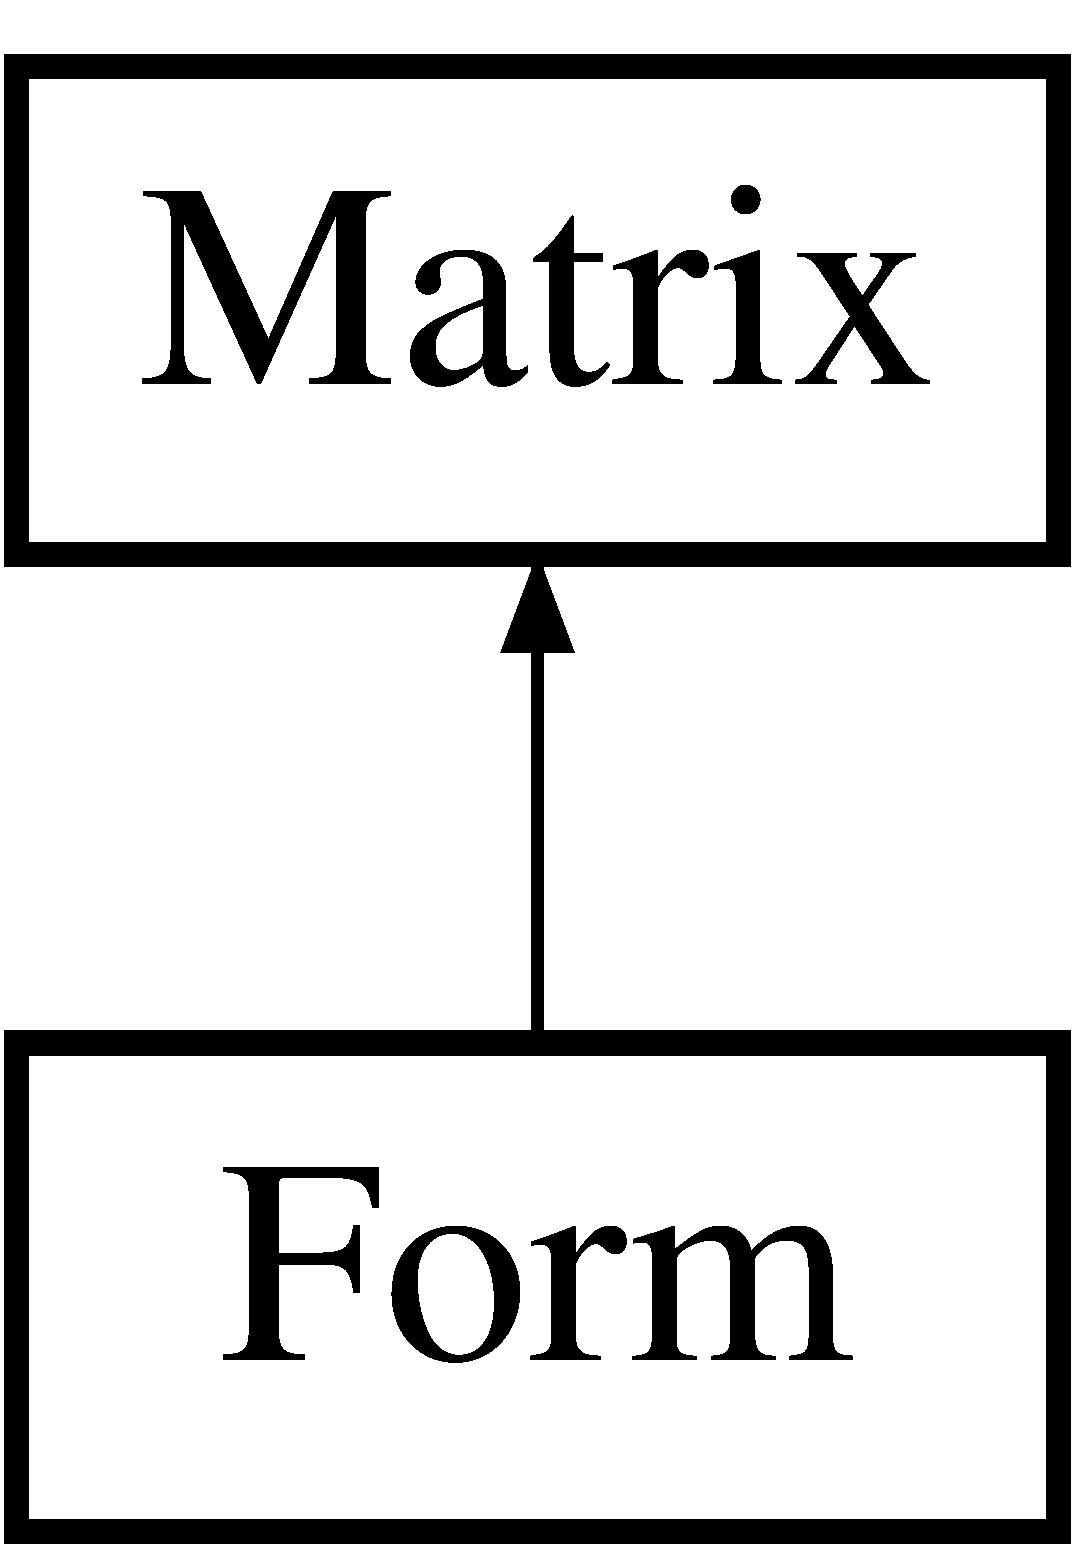
\includegraphics[height=2.000000cm]{classForm}
\end{center}
\end{figure}
\subsection*{Public Member Functions}
\begin{DoxyCompactItemize}
\item 
\hypertarget{classForm_a918137d720fb6740e8d91b5355023e3e}{
{\bfseries \_\-\_\-construct} (\$data=array())}
\label{classForm_a918137d720fb6740e8d91b5355023e3e}

\item 
\hypertarget{classForm_a0d2f1545bc27ebcaaab84baca3b2ec3d}{
{\bfseries setDefaults} (\$defaults)}
\label{classForm_a0d2f1545bc27ebcaaab84baca3b2ec3d}

\item 
\hypertarget{classForm_a4146c9fec58751931eeeafb6a5032109}{
{\bfseries setErrors} (\$errors)}
\label{classForm_a4146c9fec58751931eeeafb6a5032109}

\item 
\hypertarget{classForm_ad628bf69f4aacf56874e228f4dffe278}{
{\bfseries addErrors} (\$field, \$errors)}
\label{classForm_ad628bf69f4aacf56874e228f4dffe278}

\item 
\hypertarget{classForm_a76a626645b5dd91fea35238c40b73057}{
{\bfseries addError} (\$field, \$error)}
\label{classForm_a76a626645b5dd91fea35238c40b73057}

\item 
\hypertarget{classForm_a1cd7191ba1fab1817ea6bffab804f82d}{
{\bfseries errors} (\$field=null)}
\label{classForm_a1cd7191ba1fab1817ea6bffab804f82d}

\item 
\hyperlink{classForm_a30692b7cf24078d8ce209b98fd27aa80}{get} (\$field=null)
\item 
\hypertarget{classForm_a89ce95b4a8eacc465730fb5e240ff66d}{
{\bfseries validate} ()}
\label{classForm_a89ce95b4a8eacc465730fb5e240ff66d}

\item 
\hypertarget{classForm_a719fa0e86b18283faee39d7e0d69957d}{
{\bfseries valid} (\$field=null)}
\label{classForm_a719fa0e86b18283faee39d7e0d69957d}

\item 
\hypertarget{classForm_a29e82a4cae1e8a22abad773b8c2b2b02}{
{\bfseries \_\-\_\-get} (\$name)}
\label{classForm_a29e82a4cae1e8a22abad773b8c2b2b02}

\item 
\hypertarget{classForm_a1e913aa59b9ea8d8007c47f989558943}{
{\bfseries open} (\$formName, \$action=null, \$method= 'POST', \$attrs=array())}
\label{classForm_a1e913aa59b9ea8d8007c47f989558943}

\item 
\hypertarget{classForm_aaa8d1ff2d98b23893bfa66ae8766212a}{
{\bfseries close} ()}
\label{classForm_aaa8d1ff2d98b23893bfa66ae8766212a}

\item 
\hypertarget{classForm_a926ffa6cfcb6b0df448fdb3d084f3a85}{
{\bfseries errors} (\$field)}
\label{classForm_a926ffa6cfcb6b0df448fdb3d084f3a85}

\item 
\hypertarget{classForm_ad346f6535dce3b737a354ec158fc56b8}{
{\bfseries input} (\$name, \$attrs=array())}
\label{classForm_ad346f6535dce3b737a354ec158fc56b8}

\item 
\hyperlink{classForm_a3c7226192b6c4a6d098db567dc00fba1}{hidden} (\$name, \$attrs=array())
\item 
\hyperlink{classForm_a7856398bee38d7cc0a5e805079651725}{text} (\$name, \$attrs=array())
\item 
\hyperlink{classForm_a88fa3b1b21917530621c45e121c6e273}{password} (\$name, \$attrs=array())
\item 
\hyperlink{classForm_ab5a5c2d036613181c1fd69356bf9ac7f}{checkbox} (\$name, \$attrs=array())
\item 
\hyperlink{classForm_a3394ae873b4192b6f3827dae49bb3ee1}{radio} (\$name, \$value, \$attrs=array())
\item 
\hyperlink{classForm_a2ce53f56957c430f52afed0f7a8b900f}{textarea} (\$name, \$attrs=array())
\item 
\hyperlink{classForm_a4721ca44be121370629b04e364c70a41}{select} (\$name, \$options, \$attrs=array())
\item 
\hypertarget{classForm_a88892a17eb246d0309419b7289be9ceb}{
{\bfseries submit} (\$value=null, \$attrs=array())}
\label{classForm_a88892a17eb246d0309419b7289be9ceb}

\item 
\hyperlink{classForm_a66e9d055a0daa51aa1c5b4dd62f3f82b}{selectHour24} (\$name, \$attrs=array())
\item 
\hyperlink{classForm_ae1d9a2ca2ec79f9cf872014397447273}{selectMinute} (\$name, \$attrs=array())
\item 
\hyperlink{classForm_aea60ffaa701fea429e51ceddb3712298}{selectYesNo} (\$name, \$attrs=array())
\item 
\hypertarget{classForm_ab47a12ae2f9f2cb205de386aa259bbc8}{
{\bfseries \_\-\_\-call} (\$method, \$args)}
\label{classForm_ab47a12ae2f9f2cb205de386aa259bbc8}

\end{DoxyCompactItemize}
\subsection*{Static Public Member Functions}
\begin{DoxyCompactItemize}
\item 
static \hyperlink{classForm_afe6750a98993c81da710af555a6ec3f7}{name} ()
\item 
static \hyperlink{classForm_a51c909fa03f961faadc70d1f8121e656}{compatible} (\$data, \$allowExtraFields=false)
\end{DoxyCompactItemize}
\subsection*{Protected Attributes}
\begin{DoxyCompactItemize}
\item 
\hyperlink{classForm_a25f4ad782d570833cbd0320fd949651c}{\$\_\-defaults}
\item 
\hypertarget{classForm_a6588411906ebc9b77538fd35c66b6061}{
{\bfseries \$\_\-errors} = array()}
\label{classForm_a6588411906ebc9b77538fd35c66b6061}

\item 
\hypertarget{classForm_a99adb61969412070e68825ee27977a82}{
{\bfseries \$\_\-Form}}
\label{classForm_a99adb61969412070e68825ee27977a82}

\end{DoxyCompactItemize}
\subsection*{Static Protected Attributes}
\begin{DoxyCompactItemize}
\item 
\hypertarget{classForm_a2ae01dc28ade07ea33443d58e1f3ff35}{
static {\bfseries \$\_\-fields} = array()}
\label{classForm_a2ae01dc28ade07ea33443d58e1f3ff35}

\item 
\hypertarget{classForm_ae7b9bcff478aa176d7cbc6ad31cf0224}{
static {\bfseries \$\_\-validate} = array()}
\label{classForm_ae7b9bcff478aa176d7cbc6ad31cf0224}

\item 
\hypertarget{classForm_a10c62b840cbdcdab634fa121b935c03f}{
static {\bfseries \$\_\-requiredPresent} = array()}
\label{classForm_a10c62b840cbdcdab634fa121b935c03f}

\end{DoxyCompactItemize}


\subsection{Detailed Description}
Base \hyperlink{classFrawst}{Frawst} \hyperlink{classForm}{Form} class

This class can be extended to rigidly define properties of your application's FORMs. This allows separation of form validation from your controller logic, and prevents duplication of form processing if you use the same form in multiple areas of your site. It also helps protect against XSS by ensuring no additional fields are passed in (as long as you check for compatibility before using the form) and all required fields are present.

This class is NOT used to output form markup! For that, you can use the \hyperlink{classForm}{Form} helper. Simply pass the name of your \hyperlink{classForm}{Form} class in the open() method, and the fields will be (re)populated automatically. 

\subsection{Member Function Documentation}
\hypertarget{classForm_ab5a5c2d036613181c1fd69356bf9ac7f}{
\index{Form@{Form}!checkbox@{checkbox}}
\index{checkbox@{checkbox}!Form@{Form}}
\subsubsection[{checkbox}]{\setlength{\rightskip}{0pt plus 5cm}Form::checkbox (
\begin{DoxyParamCaption}
\item[{\$}]{ name, }
\item[{\$}]{ attrs = {\ttfamily array()}}
\end{DoxyParamCaption}
)}}
\label{classForm_ab5a5c2d036613181c1fd69356bf9ac7f}
Checkbox \hypertarget{classForm_a51c909fa03f961faadc70d1f8121e656}{
\index{Form@{Form}!compatible@{compatible}}
\index{compatible@{compatible}!Form@{Form}}
\subsubsection[{compatible}]{\setlength{\rightskip}{0pt plus 5cm}static Form::compatible (
\begin{DoxyParamCaption}
\item[{\$}]{ data, }
\item[{\$}]{ allowExtraFields = {\ttfamily false}}
\end{DoxyParamCaption}
)\hspace{0.3cm}{\ttfamily  \mbox{[}static\mbox{]}}}}
\label{classForm_a51c909fa03f961faadc70d1f8121e656}
Determines whether or not the given data is compatible with this form. 
\begin{DoxyParams}{Parameters}
\item[{\em array}]\$data \end{DoxyParams}
\begin{DoxyReturn}{Returns}
bool 
\end{DoxyReturn}
\hypertarget{classForm_a30692b7cf24078d8ce209b98fd27aa80}{
\index{Form@{Form}!get@{get}}
\index{get@{get}!Form@{Form}}
\subsubsection[{get}]{\setlength{\rightskip}{0pt plus 5cm}Form::get (
\begin{DoxyParamCaption}
\item[{\$}]{ field = {\ttfamily null}}
\end{DoxyParamCaption}
)}}
\label{classForm_a30692b7cf24078d8ce209b98fd27aa80}
If a value does not exist in the form data, use the default value instead. 

Reimplemented from \hyperlink{classMatrix}{Matrix}.

\hypertarget{classForm_a3c7226192b6c4a6d098db567dc00fba1}{
\index{Form@{Form}!hidden@{hidden}}
\index{hidden@{hidden}!Form@{Form}}
\subsubsection[{hidden}]{\setlength{\rightskip}{0pt plus 5cm}Form::hidden (
\begin{DoxyParamCaption}
\item[{\$}]{ name, }
\item[{\$}]{ attrs = {\ttfamily array()}}
\end{DoxyParamCaption}
)}}
\label{classForm_a3c7226192b6c4a6d098db567dc00fba1}
Hidden \hypertarget{classForm_afe6750a98993c81da710af555a6ec3f7}{
\index{Form@{Form}!name@{name}}
\index{name@{name}!Form@{Form}}
\subsubsection[{name}]{\setlength{\rightskip}{0pt plus 5cm}static Form::name (
\begin{DoxyParamCaption}
{}
\end{DoxyParamCaption}
)\hspace{0.3cm}{\ttfamily  \mbox{[}static\mbox{]}}}}
\label{classForm_afe6750a98993c81da710af555a6ec3f7}
Returns the form name \hypertarget{classForm_a88fa3b1b21917530621c45e121c6e273}{
\index{Form@{Form}!password@{password}}
\index{password@{password}!Form@{Form}}
\subsubsection[{password}]{\setlength{\rightskip}{0pt plus 5cm}Form::password (
\begin{DoxyParamCaption}
\item[{\$}]{ name, }
\item[{\$}]{ attrs = {\ttfamily array()}}
\end{DoxyParamCaption}
)}}
\label{classForm_a88fa3b1b21917530621c45e121c6e273}
Password \hypertarget{classForm_a3394ae873b4192b6f3827dae49bb3ee1}{
\index{Form@{Form}!radio@{radio}}
\index{radio@{radio}!Form@{Form}}
\subsubsection[{radio}]{\setlength{\rightskip}{0pt plus 5cm}Form::radio (
\begin{DoxyParamCaption}
\item[{\$}]{ name, }
\item[{\$}]{ value, }
\item[{\$}]{ attrs = {\ttfamily array()}}
\end{DoxyParamCaption}
)}}
\label{classForm_a3394ae873b4192b6f3827dae49bb3ee1}
Radio \hypertarget{classForm_a4721ca44be121370629b04e364c70a41}{
\index{Form@{Form}!select@{select}}
\index{select@{select}!Form@{Form}}
\subsubsection[{select}]{\setlength{\rightskip}{0pt plus 5cm}Form::select (
\begin{DoxyParamCaption}
\item[{\$}]{ name, }
\item[{\$}]{ options, }
\item[{\$}]{ attrs = {\ttfamily array()}}
\end{DoxyParamCaption}
)}}
\label{classForm_a4721ca44be121370629b04e364c70a41}
Select \hypertarget{classForm_a66e9d055a0daa51aa1c5b4dd62f3f82b}{
\index{Form@{Form}!selectHour24@{selectHour24}}
\index{selectHour24@{selectHour24}!Form@{Form}}
\subsubsection[{selectHour24}]{\setlength{\rightskip}{0pt plus 5cm}Form::selectHour24 (
\begin{DoxyParamCaption}
\item[{\$}]{ name, }
\item[{\$}]{ attrs = {\ttfamily array()}}
\end{DoxyParamCaption}
)}}
\label{classForm_a66e9d055a0daa51aa1c5b4dd62f3f82b}
Select box for 24 hours \hypertarget{classForm_ae1d9a2ca2ec79f9cf872014397447273}{
\index{Form@{Form}!selectMinute@{selectMinute}}
\index{selectMinute@{selectMinute}!Form@{Form}}
\subsubsection[{selectMinute}]{\setlength{\rightskip}{0pt plus 5cm}Form::selectMinute (
\begin{DoxyParamCaption}
\item[{\$}]{ name, }
\item[{\$}]{ attrs = {\ttfamily array()}}
\end{DoxyParamCaption}
)}}
\label{classForm_ae1d9a2ca2ec79f9cf872014397447273}
Select box for 60 minutes \hypertarget{classForm_aea60ffaa701fea429e51ceddb3712298}{
\index{Form@{Form}!selectYesNo@{selectYesNo}}
\index{selectYesNo@{selectYesNo}!Form@{Form}}
\subsubsection[{selectYesNo}]{\setlength{\rightskip}{0pt plus 5cm}Form::selectYesNo (
\begin{DoxyParamCaption}
\item[{\$}]{ name, }
\item[{\$}]{ attrs = {\ttfamily array()}}
\end{DoxyParamCaption}
)}}
\label{classForm_aea60ffaa701fea429e51ceddb3712298}
Yes/no select box (returns 1 for yes, 0 for no) \hypertarget{classForm_a7856398bee38d7cc0a5e805079651725}{
\index{Form@{Form}!text@{text}}
\index{text@{text}!Form@{Form}}
\subsubsection[{text}]{\setlength{\rightskip}{0pt plus 5cm}Form::text (
\begin{DoxyParamCaption}
\item[{\$}]{ name, }
\item[{\$}]{ attrs = {\ttfamily array()}}
\end{DoxyParamCaption}
)}}
\label{classForm_a7856398bee38d7cc0a5e805079651725}
Text \hypertarget{classForm_a2ce53f56957c430f52afed0f7a8b900f}{
\index{Form@{Form}!textarea@{textarea}}
\index{textarea@{textarea}!Form@{Form}}
\subsubsection[{textarea}]{\setlength{\rightskip}{0pt plus 5cm}Form::textarea (
\begin{DoxyParamCaption}
\item[{\$}]{ name, }
\item[{\$}]{ attrs = {\ttfamily array()}}
\end{DoxyParamCaption}
)}}
\label{classForm_a2ce53f56957c430f52afed0f7a8b900f}
Textarea 

\subsection{Member Data Documentation}
\hypertarget{classForm_a25f4ad782d570833cbd0320fd949651c}{
\index{Form@{Form}!\$\_\-defaults@{\$\_\-defaults}}
\index{\$\_\-defaults@{\$\_\-defaults}!Form@{Form}}
\subsubsection[{\$\_\-defaults}]{\setlength{\rightskip}{0pt plus 5cm}Form::\$\_\-defaults\hspace{0.3cm}{\ttfamily  \mbox{[}protected\mbox{]}}}}
\label{classForm_a25f4ad782d570833cbd0320fd949651c}
Default data for repopulating form fields. Keys should be in expanded format.  array 

The documentation for this class was generated from the following files:\begin{DoxyCompactItemize}
\item 
Form.php\item 
Helper/Form.php\end{DoxyCompactItemize}

\hypertarget{classFrawst}{
\section{Frawst Class Reference}
\label{classFrawst}\index{Frawst@{Frawst}}
}
Inheritance diagram for Frawst:\begin{figure}[H]
\begin{center}
\leavevmode
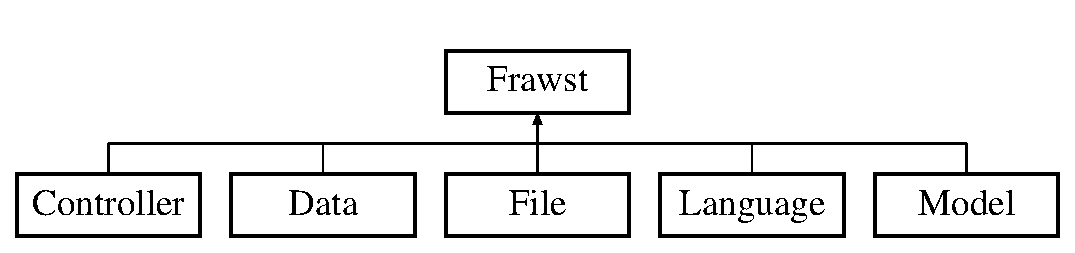
\includegraphics[height=2.000000cm]{classFrawst}
\end{center}
\end{figure}


The documentation for this class was generated from the following file:\begin{DoxyCompactItemize}
\item 
libs/Exception/Frawst.php\end{DoxyCompactItemize}

\hypertarget{classHelper}{
\section{Helper Class Reference}
\label{classHelper}\index{Helper@{Helper}}
}
Inheritance diagram for Helper:\begin{figure}[H]
\begin{center}
\leavevmode
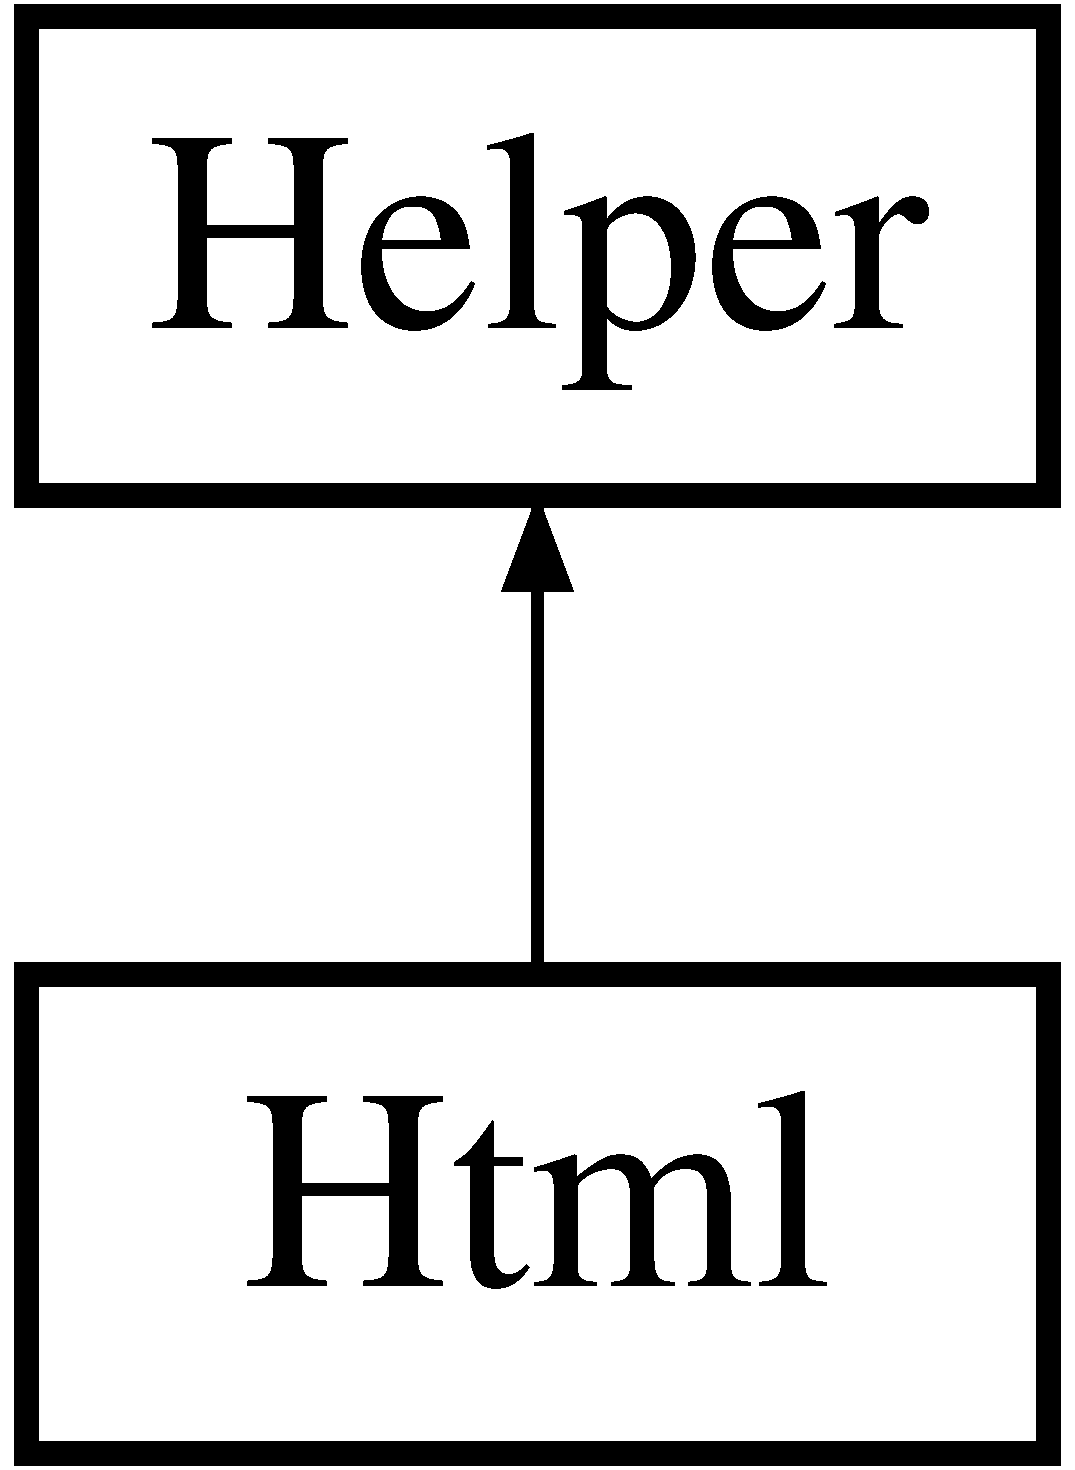
\includegraphics[height=2.000000cm]{classHelper}
\end{center}
\end{figure}
\subsection*{Public Member Functions}
\begin{DoxyCompactItemize}
\item 
\hypertarget{classHelper_aaf7c48c91d7e53584b2f2d7e4cc655f2}{
{\bfseries \_\-\_\-construct} (\$view)}
\label{classHelper_aaf7c48c91d7e53584b2f2d7e4cc655f2}

\item 
\hypertarget{classHelper_af701de06437a148a3d0633924b723ee9}{
{\bfseries \_\-\_\-get} (\$name)}
\label{classHelper_af701de06437a148a3d0633924b723ee9}

\end{DoxyCompactItemize}
\subsection*{Static Public Member Functions}
\begin{DoxyCompactItemize}
\item 
\hypertarget{classHelper_a585a3be9064e2011a3f02b9e77ae1176}{
static {\bfseries parseAttributes} (\$attrs)}
\label{classHelper_a585a3be9064e2011a3f02b9e77ae1176}

\end{DoxyCompactItemize}
\subsection*{Protected Member Functions}
\begin{DoxyCompactItemize}
\item 
\hypertarget{classHelper_adbf673fb3f7c3b1ecd20e4815ed97af1}{
{\bfseries \_\-init} ()}
\label{classHelper_adbf673fb3f7c3b1ecd20e4815ed97af1}

\end{DoxyCompactItemize}
\subsection*{Protected Attributes}
\begin{DoxyCompactItemize}
\item 
\hypertarget{classHelper_a700e3c0f47edc5c9f927e5b2b6a0fbf3}{
{\bfseries \$\_\-View}}
\label{classHelper_a700e3c0f47edc5c9f927e5b2b6a0fbf3}

\end{DoxyCompactItemize}


The documentation for this class was generated from the following file:\begin{DoxyCompactItemize}
\item 
libs/Helper.php\end{DoxyCompactItemize}

\hypertarget{classHierarchy}{
\section{Hierarchy Class Reference}
\label{classHierarchy}\index{Hierarchy@{Hierarchy}}
}
Inheritance diagram for Hierarchy:\begin{figure}[H]
\begin{center}
\leavevmode
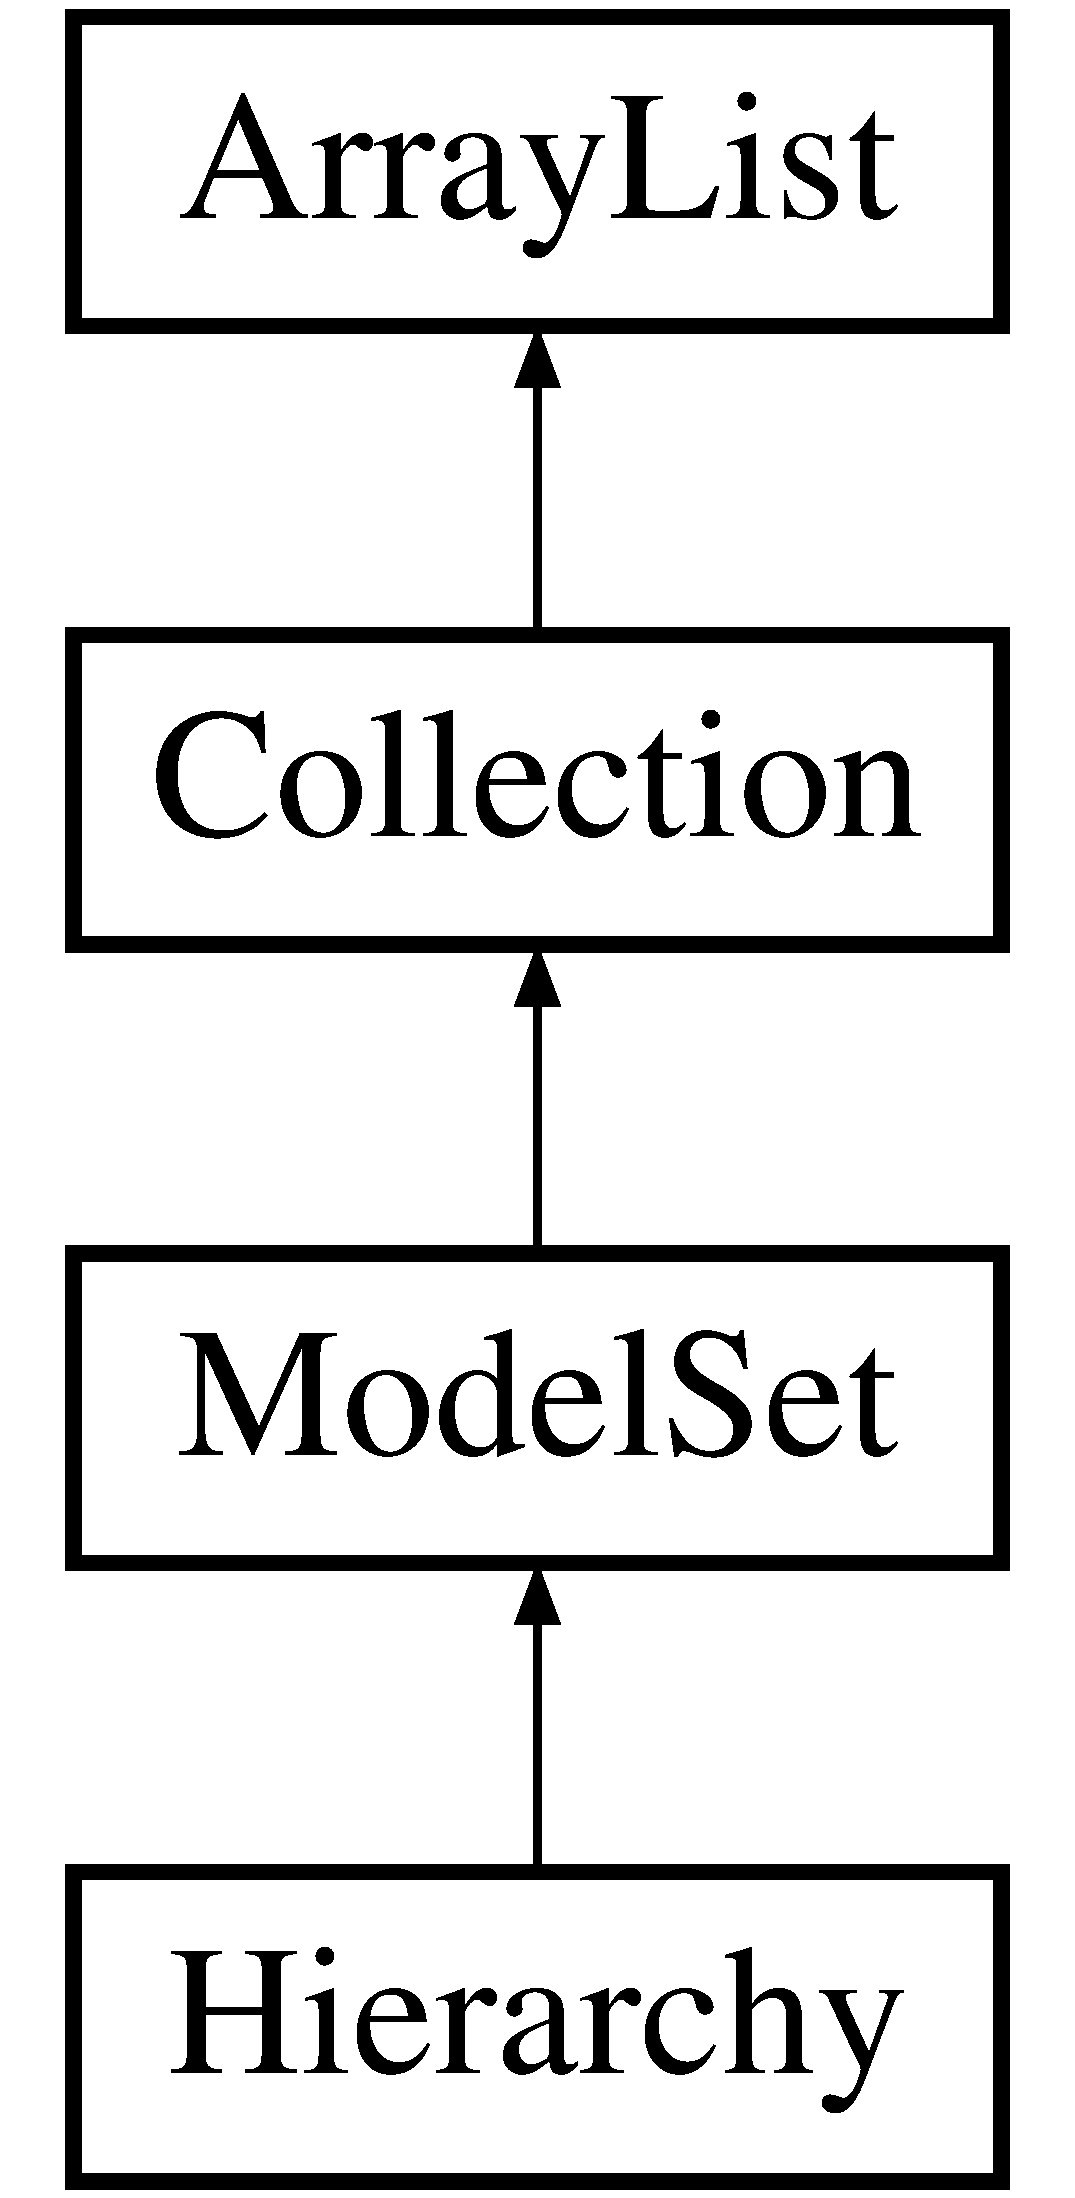
\includegraphics[height=4.000000cm]{classHierarchy}
\end{center}
\end{figure}
\subsection*{Public Member Functions}
\begin{DoxyCompactItemize}
\item 
\hyperlink{classHierarchy_a6bd1635911af5bd6472b060f177c841a}{\_\-\_\-construct} (\$type, \$roots=array())
\item 
\hyperlink{classHierarchy_a51c0b25ea641b1de5c72dca9a8a992c5}{childrenOf} (\$id, \$deep=false)
\item 
\hyperlink{classHierarchy_a7334e9be19629ef54f19e71ed3cf413b}{parentOf} (\$id)
\item 
\hyperlink{classHierarchy_ad54d88d65797331b1e6aebdd2a61c23b}{pathTo} (\$id, \$includeThis=true)
\end{DoxyCompactItemize}
\subsection*{Protected Attributes}
\begin{DoxyCompactItemize}
\item 
\hypertarget{classHierarchy_a8e4a8dea319d86aa81f82b0526be4bcc}{
{\bfseries \$\_\-structure}}
\label{classHierarchy_a8e4a8dea319d86aa81f82b0526be4bcc}

\item 
\hypertarget{classHierarchy_a92e8aa798f924f01a4cf4bd98dc56908}{
{\bfseries \$\_\-lookup}}
\label{classHierarchy_a92e8aa798f924f01a4cf4bd98dc56908}

\end{DoxyCompactItemize}


\subsection{Detailed Description}
Hierarchy-\/based model collection class to allow for easy hierarchy management and caching (automatically pulls all children recursively). Assumes your model has a self-\/referencing hasMany relationship aliased \char`\"{}Children.\char`\"{} 

\subsection{Constructor \& Destructor Documentation}
\hypertarget{classHierarchy_a6bd1635911af5bd6472b060f177c841a}{
\index{Hierarchy@{Hierarchy}!\_\-\_\-construct@{\_\-\_\-construct}}
\index{\_\-\_\-construct@{\_\-\_\-construct}!Hierarchy@{Hierarchy}}
\subsubsection[{\_\-\_\-construct}]{\setlength{\rightskip}{0pt plus 5cm}Hierarchy::\_\-\_\-construct (
\begin{DoxyParamCaption}
\item[{\$}]{ type, }
\item[{\$}]{ roots = {\ttfamily array()}}
\end{DoxyParamCaption}
)}}
\label{classHierarchy_a6bd1635911af5bd6472b060f177c841a}
If a \hyperlink{classModelSet}{ModelSet} is passed as the first parameter, the type will be automatically pulled from the \hyperlink{classModelSet}{ModelSet}. 

Reimplemented from \hyperlink{classModelSet}{ModelSet}.



\subsection{Member Function Documentation}
\hypertarget{classHierarchy_a51c0b25ea641b1de5c72dca9a8a992c5}{
\index{Hierarchy@{Hierarchy}!childrenOf@{childrenOf}}
\index{childrenOf@{childrenOf}!Hierarchy@{Hierarchy}}
\subsubsection[{childrenOf}]{\setlength{\rightskip}{0pt plus 5cm}Hierarchy::childrenOf (
\begin{DoxyParamCaption}
\item[{\$}]{ id, }
\item[{\$}]{ deep = {\ttfamily false}}
\end{DoxyParamCaption}
)}}
\label{classHierarchy_a51c0b25ea641b1de5c72dca9a8a992c5}
Gets the children of the specified model. If \$deep is true, will get a recursive list of children. \hypertarget{classHierarchy_a7334e9be19629ef54f19e71ed3cf413b}{
\index{Hierarchy@{Hierarchy}!parentOf@{parentOf}}
\index{parentOf@{parentOf}!Hierarchy@{Hierarchy}}
\subsubsection[{parentOf}]{\setlength{\rightskip}{0pt plus 5cm}Hierarchy::parentOf (
\begin{DoxyParamCaption}
\item[{\$}]{ id}
\end{DoxyParamCaption}
)}}
\label{classHierarchy_a7334e9be19629ef54f19e71ed3cf413b}
Returns the parent of the specified model. \hypertarget{classHierarchy_ad54d88d65797331b1e6aebdd2a61c23b}{
\index{Hierarchy@{Hierarchy}!pathTo@{pathTo}}
\index{pathTo@{pathTo}!Hierarchy@{Hierarchy}}
\subsubsection[{pathTo}]{\setlength{\rightskip}{0pt plus 5cm}Hierarchy::pathTo (
\begin{DoxyParamCaption}
\item[{\$}]{ id, }
\item[{\$}]{ includeThis = {\ttfamily true}}
\end{DoxyParamCaption}
)}}
\label{classHierarchy_ad54d88d65797331b1e6aebdd2a61c23b}
Returns the path to the specified model. 

The documentation for this class was generated from the following file:\begin{DoxyCompactItemize}
\item 
Library/Hierarchy.php\end{DoxyCompactItemize}

\hypertarget{classHtml}{
\section{Html Class Reference}
\label{classHtml}\index{Html@{Html}}
}
Inheritance diagram for Html:\begin{figure}[H]
\begin{center}
\leavevmode
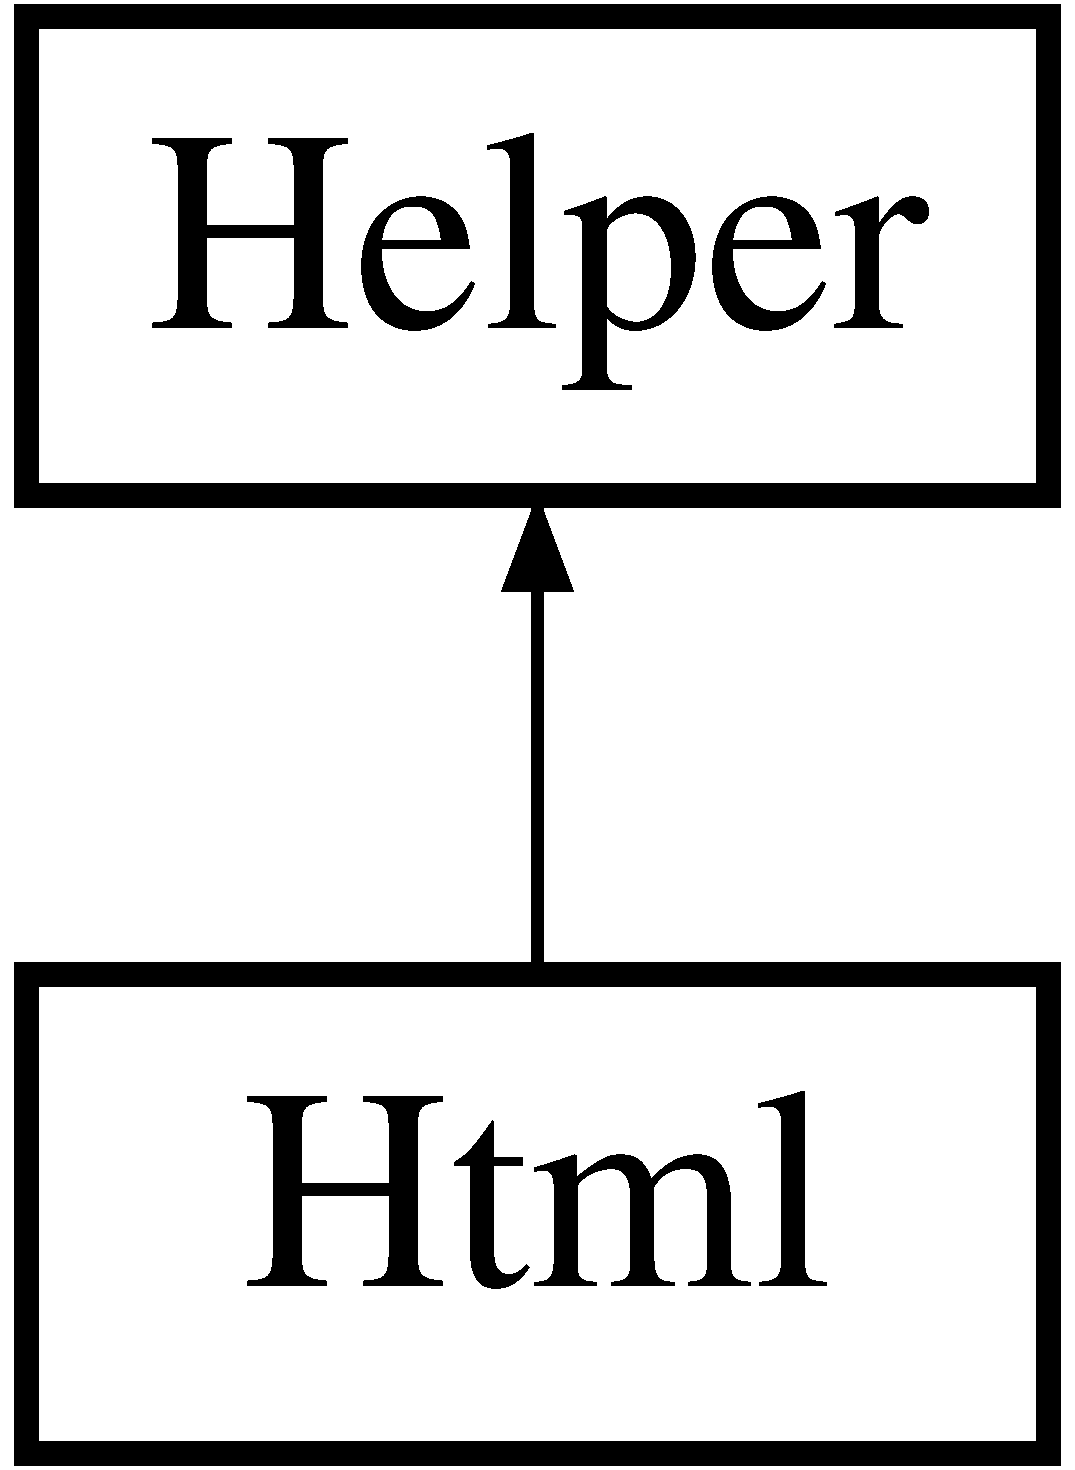
\includegraphics[height=2.000000cm]{classHtml}
\end{center}
\end{figure}
\subsection*{Public Member Functions}
\begin{DoxyCompactItemize}
\item 
\hypertarget{classHtml_ad501c8f543ea6378ea2d2bac46574844}{
{\bfseries image} (\$path, \$attrs=array())}
\label{classHtml_ad501c8f543ea6378ea2d2bac46574844}

\item 
\hypertarget{classHtml_a045fc72e96c8dbbb67cee4c5fecf317c}{
{\bfseries link} (\$uri, \$content, \$attrs=array())}
\label{classHtml_a045fc72e96c8dbbb67cee4c5fecf317c}

\item 
\hypertarget{classHtml_a5861d9dea8c77d50d35aa9ca0193f733}{
{\bfseries appLink} (\$route, \$content, \$attrs=array())}
\label{classHtml_a5861d9dea8c77d50d35aa9ca0193f733}

\item 
\hypertarget{classHtml_aeac0bac8fb00b00b933fe988f83cdb2e}{
{\bfseries sanitize} (\$string)}
\label{classHtml_aeac0bac8fb00b00b933fe988f83cdb2e}

\item 
\hypertarget{classHtml_acfbddc05d7d04905b0850a2e40e56ec2}{
{\bfseries slug} (\$string)}
\label{classHtml_acfbddc05d7d04905b0850a2e40e56ec2}

\item 
\hypertarget{classHtml_a18f421b5e12a71b28004d43e8102355f}{
{\bfseries paragraphs} (\$string)}
\label{classHtml_a18f421b5e12a71b28004d43e8102355f}

\end{DoxyCompactItemize}
\subsection*{Protected Attributes}
\begin{DoxyCompactItemize}
\item 
{\bfseries \$\_\-tags}
\end{DoxyCompactItemize}


\subsection{Member Data Documentation}
\hypertarget{classHtml_ae391dd5f6e8e263626f8ebdfd56e7e88}{
\index{Html@{Html}!\$\_\-tags@{\$\_\-tags}}
\index{\$\_\-tags@{\$\_\-tags}!Html@{Html}}
\subsubsection[{\$\_\-tags}]{\setlength{\rightskip}{0pt plus 5cm}Html::\$\_\-tags\hspace{0.3cm}{\ttfamily  \mbox{[}protected\mbox{]}}}}
\label{classHtml_ae391dd5f6e8e263626f8ebdfd56e7e88}
{\bfseries Initial value:}
\begin{DoxyCode}
 array(
                        'image' => '<img src="%s" %s>',
                        'link' => '<a href="%s" %s>%s</a>'
                )
\end{DoxyCode}


The documentation for this class was generated from the following file:\begin{DoxyCompactItemize}
\item 
Helper/Html.php\end{DoxyCompactItemize}

\hypertarget{classInflector}{
\section{Inflector Class Reference}
\label{classInflector}\index{Inflector@{Inflector}}
}
\subsection*{Static Public Member Functions}
\begin{DoxyCompactItemize}
\item 
\hypertarget{classInflector_a908104f472ffc12abdbf413907ac79e8}{
static {\bfseries upperFirst} (\$str)}
\label{classInflector_a908104f472ffc12abdbf413907ac79e8}

\item 
static \hyperlink{classInflector_a8a88a95ac17f430c6f12b84eb1248bf7}{camelCase} (\$str)
\item 
static \hyperlink{classInflector_a28be98649c8abe82e4c6dd59d8a52251}{underscore} (\$string)
\item 
static \hyperlink{classInflector_abae1c2ef023e5a0648a7a0daabba51e5}{camelBack} (\$str)
\item 
\hypertarget{classInflector_a896c15c7c8c0b1a90f56fc296c081d1f}{
static {\bfseries isUpper} (\$str)}
\label{classInflector_a896c15c7c8c0b1a90f56fc296c081d1f}

\item 
\hypertarget{classInflector_a2f6b727703c6e6e04a389154b4e74acb}{
static {\bfseries isLower} (\$str)}
\label{classInflector_a2f6b727703c6e6e04a389154b4e74acb}

\item 
\hypertarget{classInflector_afc39bbe1faba49520a80158fbdf9f2e2}{
static {\bfseries slug} (\$str)}
\label{classInflector_afc39bbe1faba49520a80158fbdf9f2e2}

\end{DoxyCompactItemize}
\subsection*{Static Protected Attributes}
\begin{DoxyCompactItemize}
\item 
\hypertarget{classInflector_aa9f0be1fd13b8c885df0f932d9b08ffb}{
static {\bfseries \$\_\-camelBack} = array()}
\label{classInflector_aa9f0be1fd13b8c885df0f932d9b08ffb}

\item 
\hypertarget{classInflector_a94b4787f78be8ac2b218e5d68278c55c}{
static {\bfseries \$\_\-underscore} = array()}
\label{classInflector_a94b4787f78be8ac2b218e5d68278c55c}

\end{DoxyCompactItemize}


\subsection{Detailed Description}
Provides various tools for manipulating strings. 

\subsection{Member Function Documentation}
\hypertarget{classInflector_abae1c2ef023e5a0648a7a0daabba51e5}{
\index{Inflector@{Inflector}!camelBack@{camelBack}}
\index{camelBack@{camelBack}!Inflector@{Inflector}}
\subsubsection[{camelBack}]{\setlength{\rightskip}{0pt plus 5cm}static Inflector::camelBack (
\begin{DoxyParamCaption}
\item[{\$}]{ str}
\end{DoxyParamCaption}
)\hspace{0.3cm}{\ttfamily  \mbox{[}static\mbox{]}}}}
\label{classInflector_abae1c2ef023e5a0648a7a0daabba51e5}
Same as camelCase, only leaves the first letter in lower-\/case (most often used for model properties).


\begin{DoxyParams}{Parameters}
\item[{\em string}]\$str The underscore string to be formatted. \end{DoxyParams}
\begin{DoxyReturn}{Returns}
string The formatted string. 
\end{DoxyReturn}
\hypertarget{classInflector_a8a88a95ac17f430c6f12b84eb1248bf7}{
\index{Inflector@{Inflector}!camelCase@{camelCase}}
\index{camelCase@{camelCase}!Inflector@{Inflector}}
\subsubsection[{camelCase}]{\setlength{\rightskip}{0pt plus 5cm}static Inflector::camelCase (
\begin{DoxyParamCaption}
\item[{\$}]{ str}
\end{DoxyParamCaption}
)\hspace{0.3cm}{\ttfamily  \mbox{[}static\mbox{]}}}}
\label{classInflector_a8a88a95ac17f430c6f12b84eb1248bf7}
Converts lower-\/case underscored words to CamelCase.


\begin{DoxyParams}{Parameters}
\item[{\em string}]\$str String to be CamelCased. \end{DoxyParams}
\begin{DoxyReturn}{Returns}
string The CamelCased string. 
\end{DoxyReturn}
\hypertarget{classInflector_a28be98649c8abe82e4c6dd59d8a52251}{
\index{Inflector@{Inflector}!underscore@{underscore}}
\index{underscore@{underscore}!Inflector@{Inflector}}
\subsubsection[{underscore}]{\setlength{\rightskip}{0pt plus 5cm}static Inflector::underscore (
\begin{DoxyParamCaption}
\item[{\$}]{ string}
\end{DoxyParamCaption}
)\hspace{0.3cm}{\ttfamily  \mbox{[}static\mbox{]}}}}
\label{classInflector_a28be98649c8abe82e4c6dd59d8a52251}
Converts CamelCase words to underscore format. This might be faster as a regex... don't feel like benchmarking right now.


\begin{DoxyParams}{Parameters}
\item[{\em string}]\$str String to be converted to underscore. \end{DoxyParams}
\begin{DoxyReturn}{Returns}
string The underscore formatted string. 
\end{DoxyReturn}


The documentation for this class was generated from the following file:\begin{DoxyCompactItemize}
\item 
libs/Library/Inflector.php\end{DoxyCompactItemize}

\hypertarget{interfaceJSONEncodable}{
\section{JSONEncodable Interface Reference}
\label{interfaceJSONEncodable}\index{JSONEncodable@{JSONEncodable}}
}
Inheritance diagram for JSONEncodable:\begin{figure}[H]
\begin{center}
\leavevmode
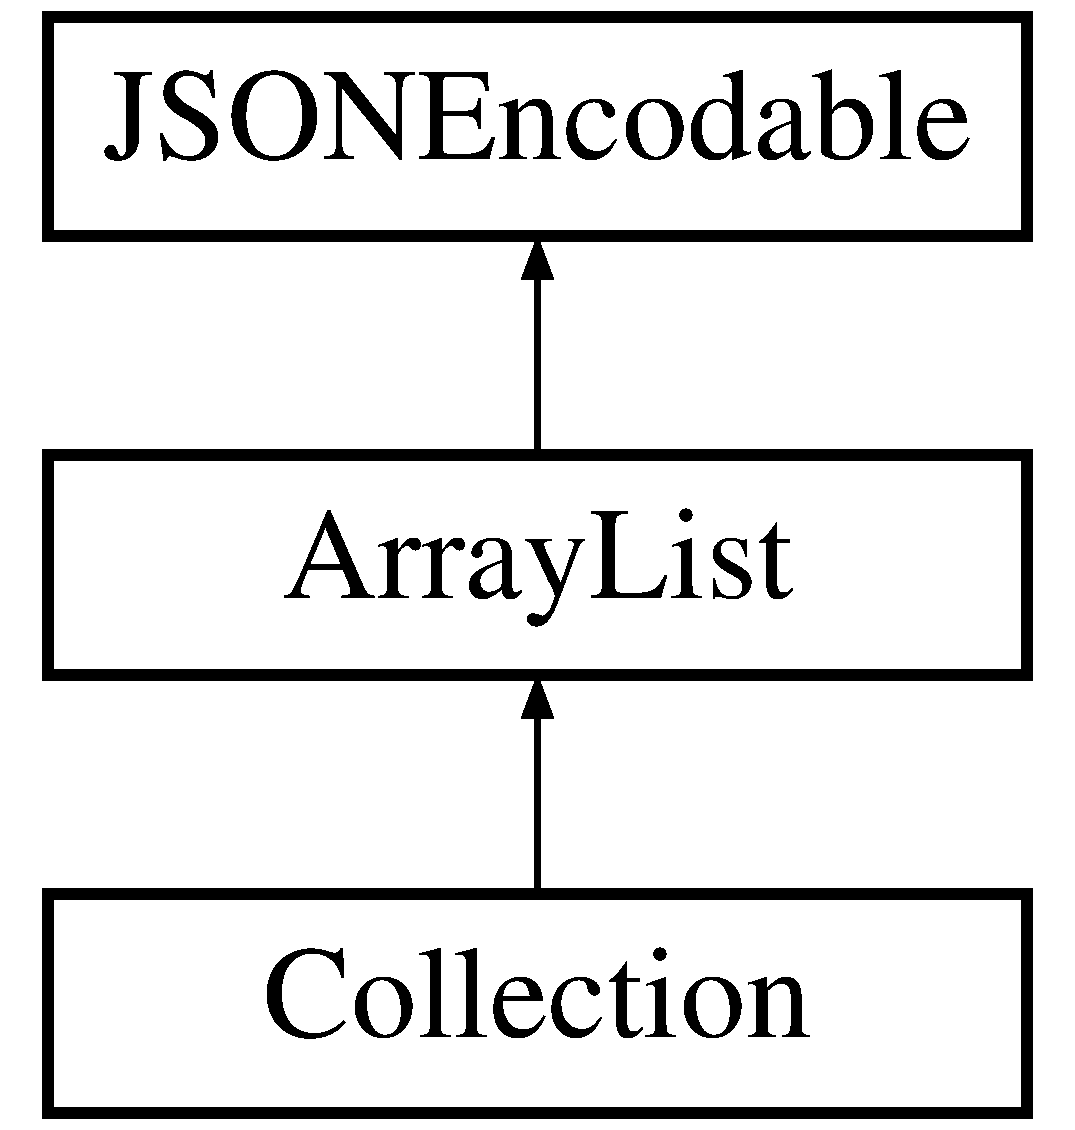
\includegraphics[height=3.000000cm]{interfaceJSONEncodable}
\end{center}
\end{figure}
\subsection*{Public Member Functions}
\begin{DoxyCompactItemize}
\item 
\hyperlink{interfaceJSONEncodable_ab9dcc56991715c542fbec7f1db0b177e}{toJSON} ()
\end{DoxyCompactItemize}


\subsection{Detailed Description}
This interface can be implemented to give more flexible JSON encoding to objects. An implementing class supplies a toJSON function that will return data to be json\_\-encode'd instead of the object itself. This can be particularly useful when protected/private properties need to be available in the encoded JSON. 

\subsection{Member Function Documentation}
\hypertarget{interfaceJSONEncodable_ab9dcc56991715c542fbec7f1db0b177e}{
\index{JSONEncodable@{JSONEncodable}!toJSON@{toJSON}}
\index{toJSON@{toJSON}!JSONEncodable@{JSONEncodable}}
\subsubsection[{toJSON}]{\setlength{\rightskip}{0pt plus 5cm}JSONEncodable::toJSON (
\begin{DoxyParamCaption}
{}
\end{DoxyParamCaption}
)}}
\label{interfaceJSONEncodable_ab9dcc56991715c542fbec7f1db0b177e}
\begin{DoxyReturn}{Returns}
mixed The data to be JSON-\/encoded 
\end{DoxyReturn}


Implemented in \hyperlink{classArrayList_ae15f74916c7173d961d6cc850776e1ae}{ArrayList}.



The documentation for this interface was generated from the following file:\begin{DoxyCompactItemize}
\item 
libs/Library/JSONEncodable.php\end{DoxyCompactItemize}

\hypertarget{classLanguage}{
\section{Language Class Reference}
\label{classLanguage}\index{Language@{Language}}
}
Inheritance diagram for Language:\begin{figure}[H]
\begin{center}
\leavevmode
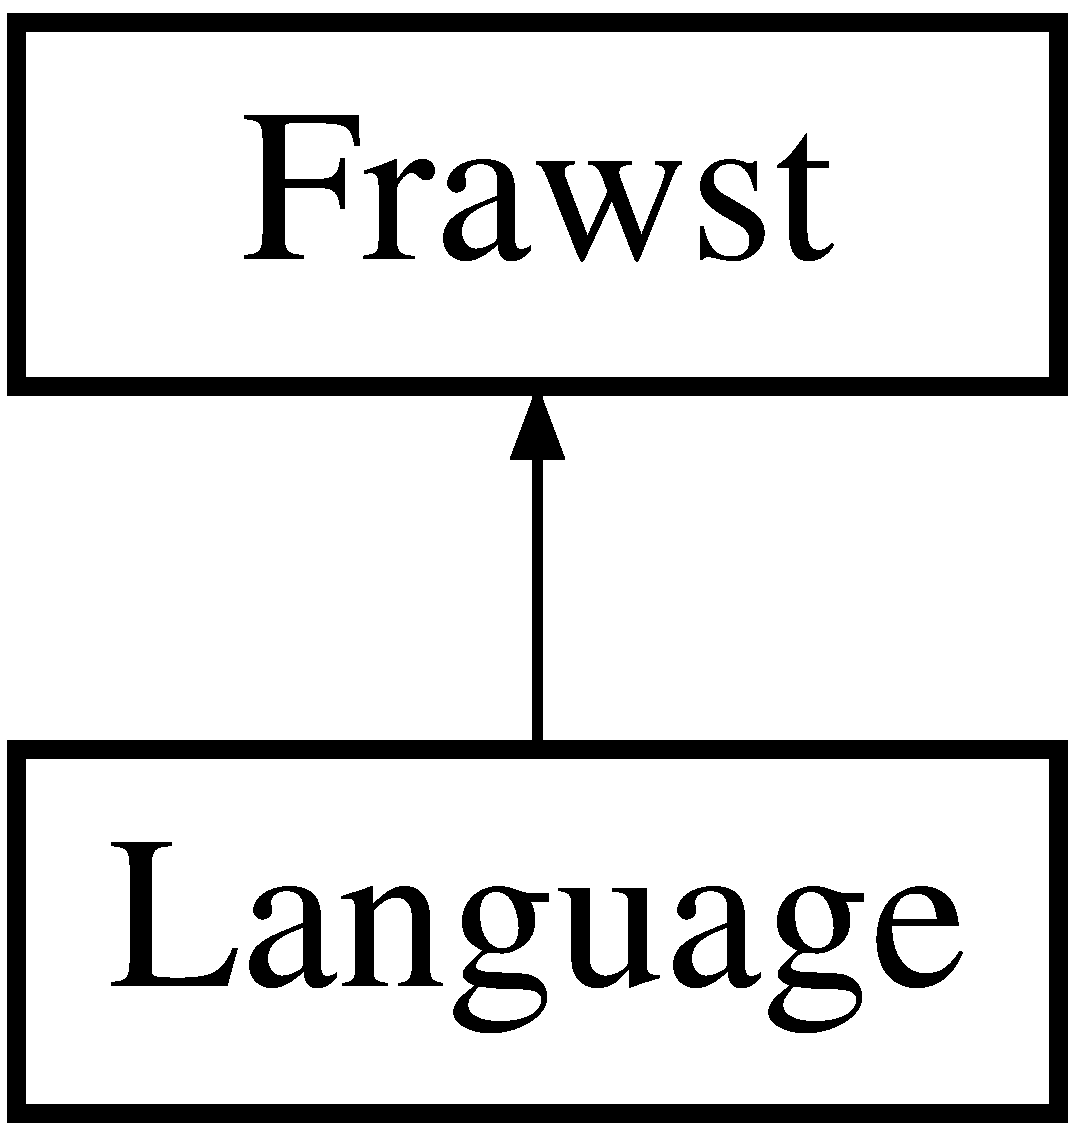
\includegraphics[height=2.000000cm]{classLanguage}
\end{center}
\end{figure}
\subsection*{Public Member Functions}
\begin{DoxyCompactItemize}
\item 
\hypertarget{classLanguage_aef959d5bc3a037220968ede228e9c8aa}{
{\bfseries \_\-\_\-construct} (\$message, \$code, \$severity, \$file, \$line)}
\label{classLanguage_aef959d5bc3a037220968ede228e9c8aa}

\end{DoxyCompactItemize}
\subsection*{Public Attributes}
\begin{DoxyCompactItemize}
\item 
\hypertarget{classLanguage_a2c142670d03c9e998b1223638fbbba3d}{
{\bfseries \$severity}}
\label{classLanguage_a2c142670d03c9e998b1223638fbbba3d}

\end{DoxyCompactItemize}


The documentation for this class was generated from the following file:\begin{DoxyCompactItemize}
\item 
libs/Exception/Language.php\end{DoxyCompactItemize}

\hypertarget{classLoader}{
\section{Loader Class Reference}
\label{classLoader}\index{Loader@{Loader}}
}
\subsection*{Static Public Member Functions}
\begin{DoxyCompactItemize}
\item 
static \hyperlink{classLoader_ad2dd2d67999331fbbc1adcc786b86bb3}{addPath} (\$path, \$pathType= '$\ast$', \$scope= 'priority')
\item 
static \hyperlink{classLoader_ac191c049e61b27b6bab8e5eeb8c969b2}{importPath} (\$class, \$scope=null)
\item 
static \hyperlink{classLoader_af5c5c67c31cb51fed22fd6989e5a91f0}{import} (\$class, \$scope=null)
\item 
static \hyperlink{classLoader_a24b740e80d2e38839ff3955415f43f6e}{getPaths} (\$name= '$\ast$', \$scope=null)
\end{DoxyCompactItemize}
\subsection*{Static Protected Attributes}
\begin{DoxyCompactItemize}
\item 
static {\bfseries \$\_\-paths}
\end{DoxyCompactItemize}


\subsection{Member Function Documentation}
\hypertarget{classLoader_ad2dd2d67999331fbbc1adcc786b86bb3}{
\index{Loader@{Loader}!addPath@{addPath}}
\index{addPath@{addPath}!Loader@{Loader}}
\subsubsection[{addPath}]{\setlength{\rightskip}{0pt plus 5cm}static Loader::addPath (
\begin{DoxyParamCaption}
\item[{\$}]{ path, }
\item[{\$}]{ pathType = {\ttfamily '$\ast$'}, }
\item[{\$}]{ scope = {\ttfamily 'priority'}}
\end{DoxyParamCaption}
)\hspace{0.3cm}{\ttfamily  \mbox{[}static\mbox{]}}}}
\label{classLoader_ad2dd2d67999331fbbc1adcc786b86bb3}
Adds a path to the loader.


\begin{DoxyParams}{Parameters}
\item[{\em string}]\$path An actual filesystem path \item[{\em string}]\$pathType The namespace covered by the path, $\ast$ = global namespace \item[{\em string}]\$scope The loading priority of the path. \end{DoxyParams}
\hypertarget{classLoader_a24b740e80d2e38839ff3955415f43f6e}{
\index{Loader@{Loader}!getPaths@{getPaths}}
\index{getPaths@{getPaths}!Loader@{Loader}}
\subsubsection[{getPaths}]{\setlength{\rightskip}{0pt plus 5cm}static Loader::getPaths (
\begin{DoxyParamCaption}
\item[{\$}]{ name = {\ttfamily '$\ast$'}, }
\item[{\$}]{ scope = {\ttfamily null}}
\end{DoxyParamCaption}
)\hspace{0.3cm}{\ttfamily  \mbox{[}static\mbox{]}}}}
\label{classLoader_a24b740e80d2e38839ff3955415f43f6e}
Generates an array of paths that will be checked for the given namespace, in order of their priority. 
\begin{DoxyParams}{Parameters}
\item[{\em string}]\$name The namespace to check \item[{\em string}]\$scope The scope to check, defaults to all scopes \end{DoxyParams}
\begin{DoxyReturn}{Returns}
array Array of loader paths for the given namespace, in the order they will be checked 
\end{DoxyReturn}
\hypertarget{classLoader_af5c5c67c31cb51fed22fd6989e5a91f0}{
\index{Loader@{Loader}!import@{import}}
\index{import@{import}!Loader@{Loader}}
\subsubsection[{import}]{\setlength{\rightskip}{0pt plus 5cm}static Loader::import (
\begin{DoxyParamCaption}
\item[{\$}]{ class, }
\item[{\$}]{ scope = {\ttfamily null}}
\end{DoxyParamCaption}
)\hspace{0.3cm}{\ttfamily  \mbox{[}static\mbox{]}}}}
\label{classLoader_af5c5c67c31cb51fed22fd6989e5a91f0}
Loads libraries using importPath


\begin{DoxyParams}{Parameters}
\item[{\em string}]\$class The name of the class to load \item[{\em string}]\$scope The scope to look in. If null, all scopes will be checked. \end{DoxyParams}
\begin{DoxyReturn}{Returns}
True if the library exists and is loaded, false otherwise. 
\end{DoxyReturn}
\hypertarget{classLoader_ac191c049e61b27b6bab8e5eeb8c969b2}{
\index{Loader@{Loader}!importPath@{importPath}}
\index{importPath@{importPath}!Loader@{Loader}}
\subsubsection[{importPath}]{\setlength{\rightskip}{0pt plus 5cm}static Loader::importPath (
\begin{DoxyParamCaption}
\item[{\$}]{ class, }
\item[{\$}]{ scope = {\ttfamily null}}
\end{DoxyParamCaption}
)\hspace{0.3cm}{\ttfamily  \mbox{[}static\mbox{]}}}}
\label{classLoader_ac191c049e61b27b6bab8e5eeb8c969b2}
Gets the path of a library based on added paths. Paths will be checked in order or priority, then order added, then specificity. For example, if a path is added as such:

\hyperlink{classLoader_ad2dd2d67999331fbbc1adcc786b86bb3}{Loader::addPath}('/app/includes/Some/Path', 'Some', 'app');

And the class  is loaded, priority paths will be tested first, followed by app paths and finally core paths. Paths with type Some will be checked first for a file called SomeClass.php. If not found, paths with type Some will be checked for a file called Path/SomeClass.php. Finally, paths with type $\ast$ will be checked for a file called Some/Path/SomeClass.php


\begin{DoxyParams}{Parameters}
\item[{\em string}]\$class The name of the class to be checked \item[{\em scope}]The scope to check. If null, all scopes will be checked. \end{DoxyParams}
\begin{DoxyReturn}{Returns}
The path to the requested library if it is found, or null. 
\end{DoxyReturn}


\subsection{Member Data Documentation}
\hypertarget{classLoader_ab18d27798c939ce8bd22c0146e129071}{
\index{Loader@{Loader}!\$\_\-paths@{\$\_\-paths}}
\index{\$\_\-paths@{\$\_\-paths}!Loader@{Loader}}
\subsubsection[{\$\_\-paths}]{\setlength{\rightskip}{0pt plus 5cm}Loader::\$\_\-paths\hspace{0.3cm}{\ttfamily  \mbox{[}static, protected\mbox{]}}}}
\label{classLoader_ab18d27798c939ce8bd22c0146e129071}
{\bfseries Initial value:}
\begin{DoxyCode}
 array(
                        'priority' => array(),
                        'app' => array(),
                        'core' => array()
                )
\end{DoxyCode}


The documentation for this class was generated from the following file:\begin{DoxyCompactItemize}
\item 
libs/Loader.php\end{DoxyCompactItemize}

\hypertarget{classMatrix}{
\section{Matrix Class Reference}
\label{classMatrix}\index{Matrix@{Matrix}}
}
Inheritance diagram for Matrix:\begin{figure}[H]
\begin{center}
\leavevmode
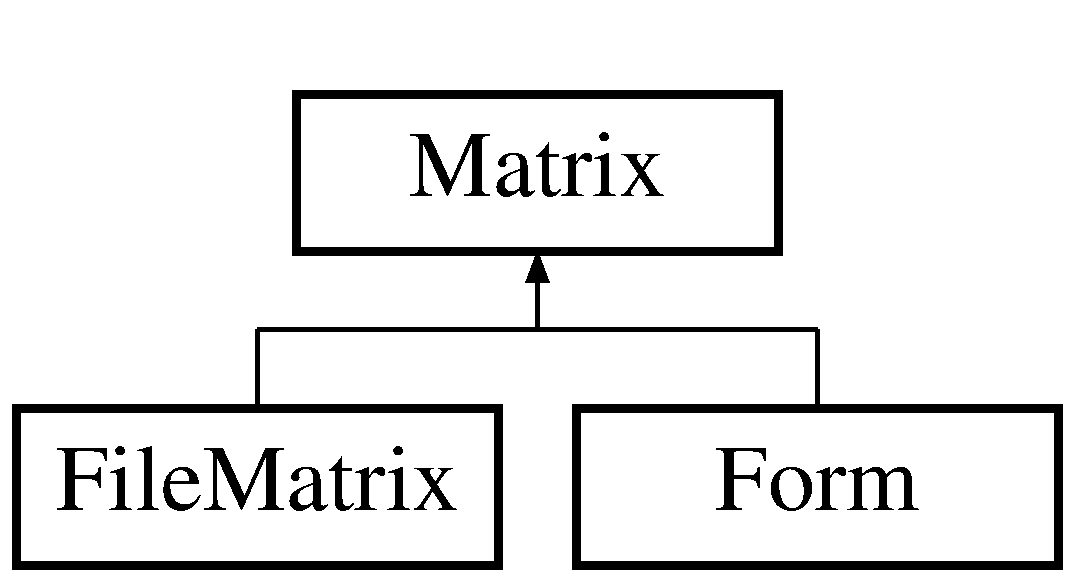
\includegraphics[height=2.000000cm]{classMatrix}
\end{center}
\end{figure}
\subsection*{Public Member Functions}
\begin{DoxyCompactItemize}
\item 
\hypertarget{classMatrix_a637568c15f5a0bc394e1455ffd25e890}{
{\bfseries \_\-\_\-construct} (\$data=array())}
\label{classMatrix_a637568c15f5a0bc394e1455ffd25e890}

\item 
\hyperlink{classMatrix_a7d0cdba14c85aa64f8e58c7b355b471f}{offsetGet} (\$offset)
\item 
\hypertarget{classMatrix_ae93338a5117b65f2c061ea077319288c}{
{\bfseries offsetSet} (\$offset, \$value)}
\label{classMatrix_ae93338a5117b65f2c061ea077319288c}

\item 
\hypertarget{classMatrix_ae202c265c3a009502e5a4bdcec57770e}{
{\bfseries offsetExists} (\$offset)}
\label{classMatrix_ae202c265c3a009502e5a4bdcec57770e}

\item 
\hypertarget{classMatrix_a26657ae4c8383f450b526f4130f4c7fd}{
{\bfseries offsetUnset} (\$offset)}
\label{classMatrix_a26657ae4c8383f450b526f4130f4c7fd}

\item 
\hypertarget{classMatrix_aa089db69c0551ab73632aeebd21fdd6c}{
{\bfseries get} (\$index=null)}
\label{classMatrix_aa089db69c0551ab73632aeebd21fdd6c}

\item 
\hypertarget{classMatrix_ab455113ea3edb53f69640adc25f56339}{
{\bfseries set} (\$index, \$value)}
\label{classMatrix_ab455113ea3edb53f69640adc25f56339}

\item 
\hypertarget{classMatrix_af536864d271ee38364bc21f823ef47cf}{
{\bfseries exists} (\$index)}
\label{classMatrix_af536864d271ee38364bc21f823ef47cf}

\item 
\hypertarget{classMatrix_aa222cc0275be3792a02411ed914e71a9}{
{\bfseries remove} (\$index)}
\label{classMatrix_aa222cc0275be3792a02411ed914e71a9}

\item 
\hypertarget{classMatrix_a97ff70dca372b9477030830150bafb74}{
{\bfseries push} (\$index, \$value)}
\label{classMatrix_a97ff70dca372b9477030830150bafb74}

\item 
\hypertarget{classMatrix_a5dbb608acffa263203b35cf5c48af596}{
{\bfseries merge} (\$index, \$array, \$recursive=false)}
\label{classMatrix_a5dbb608acffa263203b35cf5c48af596}

\end{DoxyCompactItemize}
\subsection*{Static Public Member Functions}
\begin{DoxyCompactItemize}
\item 
static \hyperlink{classMatrix_adcb5796c89a9d7eefa4acddcf83d9f20}{flatten} (\$array, \$path=null)
\item 
static \hyperlink{classMatrix_a9c51d19338f9d1e97ace7ae995292535}{expand} (\$flat)
\item 
static \hyperlink{classMatrix_ad7595b6aea73dc25a90dd72b03b99e2f}{dotToBracket} (\$dotPath, \$bracketFirst=false)
\item 
static \hyperlink{classMatrix_abf6a9524c9bb05d70b1fa94616f1fc7d}{bracketToDot} (\$bracketPath)
\item 
static \hyperlink{classMatrix_aa305f72d6665a0d17b77dafede90f208}{pathExists} (\&\$array, \$path)
\item 
static \& \hyperlink{classMatrix_aefa3e899317cb70f2ce981476c50b7ab}{pathGet} (\&\$array, \$path)
\item 
static \hyperlink{classMatrix_ad35901e861ff1f6af31d1d8745b1fc06}{pathSet} (\&\$array, \$path, \$value)
\item 
static \hyperlink{classMatrix_a7896e5ce4f773288a183e6cfe80fab56}{pathUnset} (\&\$array, \$path)
\item 
\hypertarget{classMatrix_a64b21313015529a5e9b7b6bfc0ae2283}{
static {\bfseries pathPush} (\&\$array, \$path, \$value)}
\label{classMatrix_a64b21313015529a5e9b7b6bfc0ae2283}

\item 
\hypertarget{classMatrix_a16344696c4a96a1a77f1aebb46bdecf6}{
static {\bfseries pathMerge} (\&\$array, \$path, \$merge, \$recursive=false)}
\label{classMatrix_a16344696c4a96a1a77f1aebb46bdecf6}

\end{DoxyCompactItemize}
\subsection*{Protected Attributes}
\begin{DoxyCompactItemize}
\item 
\hypertarget{classMatrix_afe54914d1576a306f59167b42c78c48c}{
{\bfseries \$\_\-data} = array()}
\label{classMatrix_afe54914d1576a306f59167b42c78c48c}

\end{DoxyCompactItemize}


\subsection{Member Function Documentation}
\hypertarget{classMatrix_abf6a9524c9bb05d70b1fa94616f1fc7d}{
\index{Matrix@{Matrix}!bracketToDot@{bracketToDot}}
\index{bracketToDot@{bracketToDot}!Matrix@{Matrix}}
\subsubsection[{bracketToDot}]{\setlength{\rightskip}{0pt plus 5cm}static Matrix::bracketToDot (
\begin{DoxyParamCaption}
\item[{\$}]{ bracketPath}
\end{DoxyParamCaption}
)\hspace{0.3cm}{\ttfamily  \mbox{[}static\mbox{]}}}}
\label{classMatrix_abf6a9524c9bb05d70b1fa94616f1fc7d}
Converts a bracket-\/separated path to a dot-\/separated path: 'User\mbox{[}name\mbox{]}\mbox{[}length\mbox{]}' -\/$>$ 'User.name.length' 
\begin{DoxyParams}{Parameters}
\item[{\em string}]\$bracketPath The bracket-\/separated path \end{DoxyParams}
\begin{DoxyReturn}{Returns}
string The dot-\/separated path 
\end{DoxyReturn}
\hypertarget{classMatrix_ad7595b6aea73dc25a90dd72b03b99e2f}{
\index{Matrix@{Matrix}!dotToBracket@{dotToBracket}}
\index{dotToBracket@{dotToBracket}!Matrix@{Matrix}}
\subsubsection[{dotToBracket}]{\setlength{\rightskip}{0pt plus 5cm}static Matrix::dotToBracket (
\begin{DoxyParamCaption}
\item[{\$}]{ dotPath, }
\item[{\$}]{ bracketFirst = {\ttfamily false}}
\end{DoxyParamCaption}
)\hspace{0.3cm}{\ttfamily  \mbox{[}static\mbox{]}}}}
\label{classMatrix_ad7595b6aea73dc25a90dd72b03b99e2f}
Parses a dot-\/separated path to a bracket-\/separated (array-\/style) path: 'User.name.length' -\/$>$ 'User\mbox{[}name\mbox{]}\mbox{[}length\mbox{]}' 
\begin{DoxyParams}{Parameters}
\item[{\em string}]\$dotPath The dot-\/separated path \item[{\em bool}]\$bracketFirst Whether or not to put brackets around the first component of the path. \end{DoxyParams}
\begin{DoxyReturn}{Returns}
string The bracket-\/separated path. 
\end{DoxyReturn}
\hypertarget{classMatrix_a9c51d19338f9d1e97ace7ae995292535}{
\index{Matrix@{Matrix}!expand@{expand}}
\index{expand@{expand}!Matrix@{Matrix}}
\subsubsection[{expand}]{\setlength{\rightskip}{0pt plus 5cm}static Matrix::expand (
\begin{DoxyParamCaption}
\item[{\$}]{ flat}
\end{DoxyParamCaption}
)\hspace{0.3cm}{\ttfamily  \mbox{[}static\mbox{]}}}}
\label{classMatrix_a9c51d19338f9d1e97ace7ae995292535}
Expands a flattened array to an n-\/dimensional matrix. \hypertarget{classMatrix_adcb5796c89a9d7eefa4acddcf83d9f20}{
\index{Matrix@{Matrix}!flatten@{flatten}}
\index{flatten@{flatten}!Matrix@{Matrix}}
\subsubsection[{flatten}]{\setlength{\rightskip}{0pt plus 5cm}static Matrix::flatten (
\begin{DoxyParamCaption}
\item[{\$}]{ array, }
\item[{\$}]{ path = {\ttfamily null}}
\end{DoxyParamCaption}
)\hspace{0.3cm}{\ttfamily  \mbox{[}static\mbox{]}}}}
\label{classMatrix_adcb5796c89a9d7eefa4acddcf83d9f20}
Returns a flattened version of the data (one-\/dimensional array with dot-\/separated paths as its keys). \hypertarget{classMatrix_a7d0cdba14c85aa64f8e58c7b355b471f}{
\index{Matrix@{Matrix}!offsetGet@{offsetGet}}
\index{offsetGet@{offsetGet}!Matrix@{Matrix}}
\subsubsection[{offsetGet}]{\setlength{\rightskip}{0pt plus 5cm}Matrix::offsetGet (
\begin{DoxyParamCaption}
\item[{\$}]{ offset}
\end{DoxyParamCaption}
)}}
\label{classMatrix_a7d0cdba14c85aa64f8e58c7b355b471f}
Required for ArrayAccess 

Reimplemented in \hyperlink{classFileMatrix_a0bd0b2818c4319b502c494d638525921}{FileMatrix}.

\hypertarget{classMatrix_aa305f72d6665a0d17b77dafede90f208}{
\index{Matrix@{Matrix}!pathExists@{pathExists}}
\index{pathExists@{pathExists}!Matrix@{Matrix}}
\subsubsection[{pathExists}]{\setlength{\rightskip}{0pt plus 5cm}static Matrix::pathExists (
\begin{DoxyParamCaption}
\item[{\&\$}]{ array, }
\item[{\$}]{ path}
\end{DoxyParamCaption}
)\hspace{0.3cm}{\ttfamily  \mbox{[}static\mbox{]}}}}
\label{classMatrix_aa305f72d6665a0d17b77dafede90f208}
Verifies that a value exists at the specified dot-\/separated path. 
\begin{DoxyParams}{Parameters}
\item[{\em array}]\$array The array to search \item[{\em string}]\$path The path to search for \end{DoxyParams}
\begin{DoxyReturn}{Returns}
bool True if the path is set, false otherwise 
\end{DoxyReturn}
\hypertarget{classMatrix_aefa3e899317cb70f2ce981476c50b7ab}{
\index{Matrix@{Matrix}!pathGet@{pathGet}}
\index{pathGet@{pathGet}!Matrix@{Matrix}}
\subsubsection[{pathGet}]{\setlength{\rightskip}{0pt plus 5cm}static\& Matrix::pathGet (
\begin{DoxyParamCaption}
\item[{\&\$}]{ array, }
\item[{\$}]{ path}
\end{DoxyParamCaption}
)\hspace{0.3cm}{\ttfamily  \mbox{[}static\mbox{]}}}}
\label{classMatrix_aefa3e899317cb70f2ce981476c50b7ab}
Finds the value at a point in a multi-\/dimensional array indicated by a dot-\/separated path; 
\begin{DoxyParams}{Parameters}
\item[{\em array}]\$array The array to search \item[{\em string}]\$path The dot-\/separated path to search for \end{DoxyParams}
\begin{DoxyReturn}{Returns}
mixed The value at the given location, by reference 
\end{DoxyReturn}
\hypertarget{classMatrix_ad35901e861ff1f6af31d1d8745b1fc06}{
\index{Matrix@{Matrix}!pathSet@{pathSet}}
\index{pathSet@{pathSet}!Matrix@{Matrix}}
\subsubsection[{pathSet}]{\setlength{\rightskip}{0pt plus 5cm}static Matrix::pathSet (
\begin{DoxyParamCaption}
\item[{\&\$}]{ array, }
\item[{\$}]{ path, }
\item[{\$}]{ value}
\end{DoxyParamCaption}
)\hspace{0.3cm}{\ttfamily  \mbox{[}static\mbox{]}}}}
\label{classMatrix_ad35901e861ff1f6af31d1d8745b1fc06}
Sets a value to an array at index indicated by a dot-\/separated path, by reference. 
\begin{DoxyParams}{Parameters}
\item[{\em array}]\$array The array to set to \item[{\em string}]\$path The dot-\/separated path to set to \item[{\em mixed}]\$value The value to set \end{DoxyParams}
\hypertarget{classMatrix_a7896e5ce4f773288a183e6cfe80fab56}{
\index{Matrix@{Matrix}!pathUnset@{pathUnset}}
\index{pathUnset@{pathUnset}!Matrix@{Matrix}}
\subsubsection[{pathUnset}]{\setlength{\rightskip}{0pt plus 5cm}static Matrix::pathUnset (
\begin{DoxyParamCaption}
\item[{\&\$}]{ array, }
\item[{\$}]{ path}
\end{DoxyParamCaption}
)\hspace{0.3cm}{\ttfamily  \mbox{[}static\mbox{]}}}}
\label{classMatrix_a7896e5ce4f773288a183e6cfe80fab56}
Unsets the specified dot-\/separated path. 
\begin{DoxyParams}{Parameters}
\item[{\em array}]\$array The array to unset from \item[{\em string}]\$path The path to unset \end{DoxyParams}


The documentation for this class was generated from the following file:\begin{DoxyCompactItemize}
\item 
Library/Matrix.php\end{DoxyCompactItemize}

\hypertarget{classModel}{
\section{Model Class Reference}
\label{classModel}\index{Model@{Model}}
}
Inheritance diagram for Model:\begin{figure}[H]
\begin{center}
\leavevmode
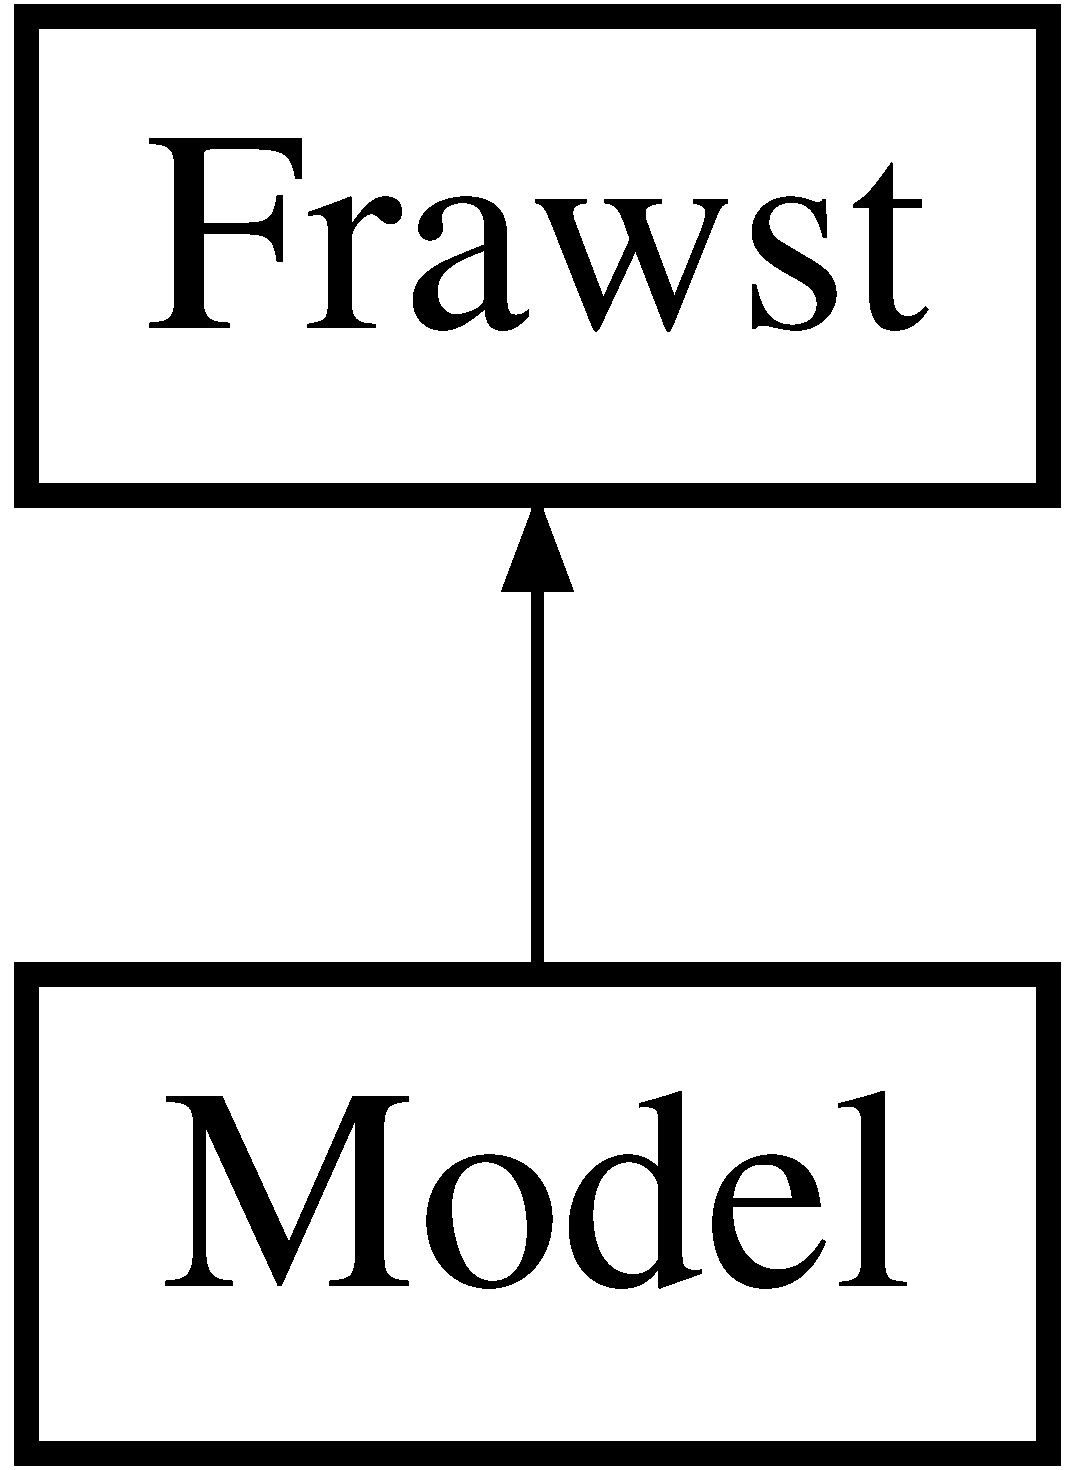
\includegraphics[height=2.000000cm]{classModel}
\end{center}
\end{figure}


The documentation for this class was generated from the following file:\begin{DoxyCompactItemize}
\item 
libs/Exception/Model.php\end{DoxyCompactItemize}

\hypertarget{classRequest}{
\section{Request Class Reference}
\label{classRequest}\index{Request@{Request}}
}
\subsection*{Public Member Functions}
\begin{DoxyCompactItemize}
\item 
\hyperlink{classRequest_af7216dd02f55fac9786612a098c6195e}{\_\-\_\-construct} (\$route, \$data=array(), \$method= 'GET', \$headers=array(), \$persist=array())
\item 
\hyperlink{classRequest_ad14cb0c1c2913fc4d86a19bfd4383dbc}{\_\-\_\-get} (\$name)
\item 
\hyperlink{classRequest_a30b1590321b7e93b6894e0ec557e46d5}{headers} ()
\item 
\hyperlink{classRequest_ac7de8477459542e9ff545cd292b7914e}{header} (\$name)
\item 
\hyperlink{classRequest_a5057f0fabb69a4c19af6e218b7b9bb7d}{isAjax} ()
\item 
\hyperlink{classRequest_aa97ca0a4c1ab78c7595a82fc8b2ec57f}{path} (\$route=null)
\item 
\hyperlink{classRequest_aeaba1ad044124a11cd68866603ce1fef}{route} (\$params=false)
\item 
\hyperlink{classRequest_a18ea75feddb5285b8097a52c78f17b2d}{subRequest} (\$route, \$data=array(), \$method= 'GET')
\item 
\hyperlink{classRequest_a7eafeed4dd7521aa654f70663d663dcf}{execute} ()
\item 
\hyperlink{classRequest_aac8d4b96b9b900a7edf41ca657ea0b6d}{method} ()
\item 
\hypertarget{classRequest_a67c4deda799d1c1d4839ed4f7830fa55}{
{\bfseries params} ()}
\label{classRequest_a67c4deda799d1c1d4839ed4f7830fa55}

\item 
\hyperlink{classRequest_a07e525938b1a92175ffe01808e070ec8}{get} (\$key=null, \$default=null)
\item 
\hyperlink{classRequest_a5439c158517f97674d201dcfe5dad11d}{post} (\$key=null, \$default=null)
\item 
\hyperlink{classRequest_af523fe9032ce728bcb27156eae258c0d}{put} (\$key=null, \$default=null)
\item 
\hyperlink{classRequest_a4a342ba4c5656bb467e43605287a8e2a}{delete} (\$key=null, \$default=null)
\item 
\hyperlink{classRequest_ac6dea526aea1f35a9f939b4b768397d8}{data} (\$key=null, \$default=null)
\item 
\hyperlink{classRequest_aa906be06b4d1c1d722727efc04d300e7}{form} (\$formName=null)
\item 
\hyperlink{classRequest_a096cae394f50b2f9be98354272c2c32e}{persist} (\$key, \$value=null)
\item 
\hyperlink{classRequest_a134ffcd200dcc73daf24b378ca056ba7}{getRuntime} ()
\end{DoxyCompactItemize}
\subsection*{Protected Attributes}
\begin{DoxyCompactItemize}
\item 
\hypertarget{classRequest_a79c93bbc226b36f8f59c3b856eb72120}{
{\bfseries \$\_\-startTime}}
\label{classRequest_a79c93bbc226b36f8f59c3b856eb72120}

\item 
\hypertarget{classRequest_ad6193d720d21be89331319dd09985c58}{
{\bfseries \$\_\-Controller}}
\label{classRequest_ad6193d720d21be89331319dd09985c58}

\item 
\hypertarget{classRequest_a81f4270e02a1a9243c32b4fb37b360a7}{
{\bfseries \$\_\-Route}}
\label{classRequest_a81f4270e02a1a9243c32b4fb37b360a7}

\item 
\hypertarget{classRequest_a52b9fd804e2fd8038f325fa7601274d2}{
{\bfseries \$\_\-headers}}
\label{classRequest_a52b9fd804e2fd8038f325fa7601274d2}

\item 
\hypertarget{classRequest_a2555f1eb5ec20322e0032fe1d0359687}{
{\bfseries \$\_\-method}}
\label{classRequest_a2555f1eb5ec20322e0032fe1d0359687}

\item 
\hypertarget{classRequest_aad7894a284ec13d0c720a9c18db06151}{
{\bfseries \$\_\-data}}
\label{classRequest_aad7894a284ec13d0c720a9c18db06151}

\item 
\hypertarget{classRequest_aba57a9def753ffdf8e5c037372df974b}{
{\bfseries \$\_\-Form}}
\label{classRequest_aba57a9def753ffdf8e5c037372df974b}

\item 
\hypertarget{classRequest_aa885eff8edc7e0361676bff6528915f6}{
{\bfseries \$\_\-Response}}
\label{classRequest_aa885eff8edc7e0361676bff6528915f6}

\item 
\hyperlink{classRequest_a6529301fb8d03a3724f00c0f625accce}{\$\_\-persist}
\end{DoxyCompactItemize}


\subsection{Detailed Description}
\hyperlink{classFrawst}{Frawst} \hyperlink{classRequest}{Request} Handler

A \hyperlink{classRequest}{Request} object simulates an HTTP request to a particular route in your application. 

\subsection{Constructor \& Destructor Documentation}
\hypertarget{classRequest_af7216dd02f55fac9786612a098c6195e}{
\index{Request@{Request}!\_\-\_\-construct@{\_\-\_\-construct}}
\index{\_\-\_\-construct@{\_\-\_\-construct}!Request@{Request}}
\subsubsection[{\_\-\_\-construct}]{\setlength{\rightskip}{0pt plus 5cm}Request::\_\-\_\-construct (
\begin{DoxyParamCaption}
\item[{\$}]{ route, }
\item[{\$}]{ data = {\ttfamily array()}, }
\item[{\$}]{ method = {\ttfamily 'GET'}, }
\item[{\$}]{ headers = {\ttfamily array()}, }
\item[{\$}]{ persist = {\ttfamily array()}}
\end{DoxyParamCaption}
)}}
\label{classRequest_af7216dd02f55fac9786612a098c6195e}
Constructor 
\begin{DoxyParams}{Parameters}
\item[{\em mixed}]\$route \item[{\em array}]\$data \item[{\em string}]\$method \item[{\em array}]\$headers \item[{\em array}]\$persist \end{DoxyParams}


\subsection{Member Function Documentation}
\hypertarget{classRequest_ad14cb0c1c2913fc4d86a19bfd4383dbc}{
\index{Request@{Request}!\_\-\_\-get@{\_\-\_\-get}}
\index{\_\-\_\-get@{\_\-\_\-get}!Request@{Request}}
\subsubsection[{\_\-\_\-get}]{\setlength{\rightskip}{0pt plus 5cm}Request::\_\-\_\-get (
\begin{DoxyParamCaption}
\item[{\$}]{ name}
\end{DoxyParamCaption}
)}}
\label{classRequest_ad14cb0c1c2913fc4d86a19bfd4383dbc}
Hacked to give the illusion of public readonly properties 
\begin{DoxyParams}{Parameters}
\item[{\em string}]\$name \end{DoxyParams}
\begin{DoxyReturn}{Returns}
object A read-\/only property 
\end{DoxyReturn}
\hypertarget{classRequest_ac6dea526aea1f35a9f939b4b768397d8}{
\index{Request@{Request}!data@{data}}
\index{data@{data}!Request@{Request}}
\subsubsection[{data}]{\setlength{\rightskip}{0pt plus 5cm}Request::data (
\begin{DoxyParamCaption}
\item[{\$}]{ key = {\ttfamily null}, }
\item[{\$}]{ default = {\ttfamily null}}
\end{DoxyParamCaption}
)}}
\label{classRequest_ac6dea526aea1f35a9f939b4b768397d8}
Returns request data 
\begin{DoxyParams}{Parameters}
\item[{\em string}]\$key A dot-\/style associative array index \item[{\em string}]\$default The value to return if the specified index was not found \end{DoxyParams}
\begin{DoxyReturn}{Returns}
mixed 
\end{DoxyReturn}
\hypertarget{classRequest_a4a342ba4c5656bb467e43605287a8e2a}{
\index{Request@{Request}!delete@{delete}}
\index{delete@{delete}!Request@{Request}}
\subsubsection[{delete}]{\setlength{\rightskip}{0pt plus 5cm}Request::delete (
\begin{DoxyParamCaption}
\item[{\$}]{ key = {\ttfamily null}, }
\item[{\$}]{ default = {\ttfamily null}}
\end{DoxyParamCaption}
)}}
\label{classRequest_a4a342ba4c5656bb467e43605287a8e2a}
Returns DELETE data. See \hyperlink{classRequest_ac6dea526aea1f35a9f939b4b768397d8}{Request::data()} for argument/return docs 
\begin{DoxyParams}{Parameters}
\item[{\em string}]\$key \item[{\em string}]\$default \end{DoxyParams}
\begin{DoxyReturn}{Returns}
array 
\end{DoxyReturn}
\hypertarget{classRequest_a7eafeed4dd7521aa654f70663d663dcf}{
\index{Request@{Request}!execute@{execute}}
\index{execute@{execute}!Request@{Request}}
\subsubsection[{execute}]{\setlength{\rightskip}{0pt plus 5cm}Request::execute (
\begin{DoxyParamCaption}
{}
\end{DoxyParamCaption}
)}}
\label{classRequest_a7eafeed4dd7521aa654f70663d663dcf}
Executes the controller action and sets the return data to this Request's response object. \begin{DoxyReturn}{Returns}
mixed The response object for this \hyperlink{classRequest}{Request} 
\end{DoxyReturn}
\hypertarget{classRequest_aa906be06b4d1c1d722727efc04d300e7}{
\index{Request@{Request}!form@{form}}
\index{form@{form}!Request@{Request}}
\subsubsection[{form}]{\setlength{\rightskip}{0pt plus 5cm}Request::form (
\begin{DoxyParamCaption}
\item[{\$}]{ formName = {\ttfamily null}}
\end{DoxyParamCaption}
)}}
\label{classRequest_aa906be06b4d1c1d722727efc04d300e7}
Returns a \hyperlink{classForm}{Form} object using the request data, if it is compatible. 
\begin{DoxyParams}{Parameters}
\item[{\em string}]\$formName The name of the form. If not provided, will check for a \_\-\_\-\_\-FORMNAME key in the request data. \end{DoxyParams}
\begin{DoxyReturn}{Returns}
\hyperlink{classFrawst}{Frawst} 
\end{DoxyReturn}
\hypertarget{classRequest_a07e525938b1a92175ffe01808e070ec8}{
\index{Request@{Request}!get@{get}}
\index{get@{get}!Request@{Request}}
\subsubsection[{get}]{\setlength{\rightskip}{0pt plus 5cm}Request::get (
\begin{DoxyParamCaption}
\item[{\$}]{ key = {\ttfamily null}, }
\item[{\$}]{ default = {\ttfamily null}}
\end{DoxyParamCaption}
)}}
\label{classRequest_a07e525938b1a92175ffe01808e070ec8}
Returns GET data. See \hyperlink{classRequest_ac6dea526aea1f35a9f939b4b768397d8}{Request::data()} for argument/return docs 
\begin{DoxyParams}{Parameters}
\item[{\em string}]\$key \item[{\em string}]\$default \end{DoxyParams}
\begin{DoxyReturn}{Returns}
array 
\end{DoxyReturn}
\hypertarget{classRequest_a134ffcd200dcc73daf24b378ca056ba7}{
\index{Request@{Request}!getRuntime@{getRuntime}}
\index{getRuntime@{getRuntime}!Request@{Request}}
\subsubsection[{getRuntime}]{\setlength{\rightskip}{0pt plus 5cm}Request::getRuntime (
\begin{DoxyParamCaption}
{}
\end{DoxyParamCaption}
)}}
\label{classRequest_a134ffcd200dcc73daf24b378ca056ba7}
\begin{DoxyReturn}{Returns}
float The runtime elapsed for this request. 
\end{DoxyReturn}
\hypertarget{classRequest_ac7de8477459542e9ff545cd292b7914e}{
\index{Request@{Request}!header@{header}}
\index{header@{header}!Request@{Request}}
\subsubsection[{header}]{\setlength{\rightskip}{0pt plus 5cm}Request::header (
\begin{DoxyParamCaption}
\item[{\$}]{ name}
\end{DoxyParamCaption}
)}}
\label{classRequest_ac7de8477459542e9ff545cd292b7914e}
Gets the value of a request header 
\begin{DoxyParams}{Parameters}
\item[{\em string}]\$name \end{DoxyParams}
\begin{DoxyReturn}{Returns}
string The value of the request header, or null if not set 
\end{DoxyReturn}
\hypertarget{classRequest_a30b1590321b7e93b6894e0ec557e46d5}{
\index{Request@{Request}!headers@{headers}}
\index{headers@{headers}!Request@{Request}}
\subsubsection[{headers}]{\setlength{\rightskip}{0pt plus 5cm}Request::headers (
\begin{DoxyParamCaption}
{}
\end{DoxyParamCaption}
)}}
\label{classRequest_a30b1590321b7e93b6894e0ec557e46d5}
\begin{DoxyReturn}{Returns}
array Associative array of request headers 
\end{DoxyReturn}
\hypertarget{classRequest_a5057f0fabb69a4c19af6e218b7b9bb7d}{
\index{Request@{Request}!isAjax@{isAjax}}
\index{isAjax@{isAjax}!Request@{Request}}
\subsubsection[{isAjax}]{\setlength{\rightskip}{0pt plus 5cm}Request::isAjax (
\begin{DoxyParamCaption}
{}
\end{DoxyParamCaption}
)}}
\label{classRequest_a5057f0fabb69a4c19af6e218b7b9bb7d}
Whether or not this request will be rendered as AJAX (layoutless) \begin{DoxyReturn}{Returns}
bool 
\end{DoxyReturn}
\hypertarget{classRequest_aac8d4b96b9b900a7edf41ca657ea0b6d}{
\index{Request@{Request}!method@{method}}
\index{method@{method}!Request@{Request}}
\subsubsection[{method}]{\setlength{\rightskip}{0pt plus 5cm}Request::method (
\begin{DoxyParamCaption}
{}
\end{DoxyParamCaption}
)}}
\label{classRequest_aac8d4b96b9b900a7edf41ca657ea0b6d}
\begin{DoxyReturn}{Returns}
string The request method (POST, GET, etc.) 
\end{DoxyReturn}
\hypertarget{classRequest_aa97ca0a4c1ab78c7595a82fc8b2ec57f}{
\index{Request@{Request}!path@{path}}
\index{path@{path}!Request@{Request}}
\subsubsection[{path}]{\setlength{\rightskip}{0pt plus 5cm}Request::path (
\begin{DoxyParamCaption}
\item[{\$}]{ route = {\ttfamily null}}
\end{DoxyParamCaption}
)}}
\label{classRequest_aa97ca0a4c1ab78c7595a82fc8b2ec57f}
Returns the full path from the web root to the given route 
\begin{DoxyParams}{Parameters}
\item[{\em string}]\$route If null, will use the current route with parameters \end{DoxyParams}
\begin{DoxyReturn}{Returns}
string The path relative to the web root 
\end{DoxyReturn}
\hypertarget{classRequest_a096cae394f50b2f9be98354272c2c32e}{
\index{Request@{Request}!persist@{persist}}
\index{persist@{persist}!Request@{Request}}
\subsubsection[{persist}]{\setlength{\rightskip}{0pt plus 5cm}Request::persist (
\begin{DoxyParamCaption}
\item[{\$}]{ key, }
\item[{\$}]{ value = {\ttfamily null}}
\end{DoxyParamCaption}
)}}
\label{classRequest_a096cae394f50b2f9be98354272c2c32e}
Get and set persistent data (passed on to sub-\/requests) 
\begin{DoxyParams}{Parameters}
\item[{\em string}]\$key A key for the data being set or retrieved \item[{\em mixed}]\$value The value being persisted \end{DoxyParams}
\begin{DoxyReturn}{Returns}
mixed The value stored under the persisted value 
\end{DoxyReturn}
\hypertarget{classRequest_a5439c158517f97674d201dcfe5dad11d}{
\index{Request@{Request}!post@{post}}
\index{post@{post}!Request@{Request}}
\subsubsection[{post}]{\setlength{\rightskip}{0pt plus 5cm}Request::post (
\begin{DoxyParamCaption}
\item[{\$}]{ key = {\ttfamily null}, }
\item[{\$}]{ default = {\ttfamily null}}
\end{DoxyParamCaption}
)}}
\label{classRequest_a5439c158517f97674d201dcfe5dad11d}
Returns POST data. See \hyperlink{classRequest_ac6dea526aea1f35a9f939b4b768397d8}{Request::data()} for argument/return docs 
\begin{DoxyParams}{Parameters}
\item[{\em string}]\$key \item[{\em string}]\$default \end{DoxyParams}
\begin{DoxyReturn}{Returns}
array 
\end{DoxyReturn}
\hypertarget{classRequest_af523fe9032ce728bcb27156eae258c0d}{
\index{Request@{Request}!put@{put}}
\index{put@{put}!Request@{Request}}
\subsubsection[{put}]{\setlength{\rightskip}{0pt plus 5cm}Request::put (
\begin{DoxyParamCaption}
\item[{\$}]{ key = {\ttfamily null}, }
\item[{\$}]{ default = {\ttfamily null}}
\end{DoxyParamCaption}
)}}
\label{classRequest_af523fe9032ce728bcb27156eae258c0d}
Returns PUT data. See \hyperlink{classRequest_ac6dea526aea1f35a9f939b4b768397d8}{Request::data()} for argument/return docs 
\begin{DoxyParams}{Parameters}
\item[{\em string}]\$key \item[{\em string}]\$default \end{DoxyParams}
\begin{DoxyReturn}{Returns}
array 
\end{DoxyReturn}
\hypertarget{classRequest_aeaba1ad044124a11cd68866603ce1fef}{
\index{Request@{Request}!route@{route}}
\index{route@{route}!Request@{Request}}
\subsubsection[{route}]{\setlength{\rightskip}{0pt plus 5cm}Request::route (
\begin{DoxyParamCaption}
\item[{\$}]{ params = {\ttfamily false}}
\end{DoxyParamCaption}
)}}
\label{classRequest_aeaba1ad044124a11cd68866603ce1fef}
Returns the resolved route of the current request. 
\begin{DoxyParams}{Parameters}
\item[{\em bool}]\$params If true, request parameters will also be appended \end{DoxyParams}
\begin{DoxyReturn}{Returns}
string The resolved route 
\end{DoxyReturn}
\hypertarget{classRequest_a18ea75feddb5285b8097a52c78f17b2d}{
\index{Request@{Request}!subRequest@{subRequest}}
\index{subRequest@{subRequest}!Request@{Request}}
\subsubsection[{subRequest}]{\setlength{\rightskip}{0pt plus 5cm}Request::subRequest (
\begin{DoxyParamCaption}
\item[{\$}]{ route, }
\item[{\$}]{ data = {\ttfamily array()}, }
\item[{\$}]{ method = {\ttfamily 'GET'}}
\end{DoxyParamCaption}
)}}
\label{classRequest_a18ea75feddb5285b8097a52c78f17b2d}
Creates a sub-\/request with the same persistent data and headers as this request, in AJAX mode. 
\begin{DoxyParams}{Parameters}
\item[{\em string}]\$route \end{DoxyParams}
\begin{DoxyReturn}{Returns}
\hyperlink{classFrawst}{Frawst} The sub-\/request object 
\end{DoxyReturn}


\subsection{Member Data Documentation}
\hypertarget{classRequest_a6529301fb8d03a3724f00c0f625accce}{
\index{Request@{Request}!\$\_\-persist@{\$\_\-persist}}
\index{\$\_\-persist@{\$\_\-persist}!Request@{Request}}
\subsubsection[{\$\_\-persist}]{\setlength{\rightskip}{0pt plus 5cm}Request::\$\_\-persist\hspace{0.3cm}{\ttfamily  \mbox{[}protected\mbox{]}}}}
\label{classRequest_a6529301fb8d03a3724f00c0f625accce}
Persistent data to be sent to sub-\/requests. 

The documentation for this class was generated from the following file:\begin{DoxyCompactItemize}
\item 
Request.php\end{DoxyCompactItemize}

\hypertarget{classResponse}{
\section{Response Class Reference}
\label{classResponse}\index{Response@{Response}}
}
\subsection*{Public Member Functions}
\begin{DoxyCompactItemize}
\item 
\hyperlink{classResponse_a0b56fd29658dadcf8b08be1912a59c0e}{\_\-\_\-construct} (\$request)
\item 
\hyperlink{classResponse_a784441c53f2d035af9cf8736006aa914}{\_\-\_\-get} (\$name)
\item 
\hyperlink{classResponse_ac4311e7d9dcec3bcdb0d55807303e7c1}{data} (\$data=null)
\item 
\hyperlink{classResponse_a007132b026abc70f7085d153c2359969}{headers} ()
\item 
\hyperlink{classResponse_ae29e05652ee532c0e1fe33f1ea91b679}{header} (\$name, \$value=null)
\item 
\hyperlink{classResponse_ab821b9432e79a01873aebee827876f8e}{redirect} (\$to= '', \$external=false)
\item 
\hyperlink{classResponse_afe4adc06ad1212cdea51f1312ad58249}{render} (\$viewClass= '\hyperlink{classFrawst}{Frawst}$\backslash$$\backslash$\hyperlink{classView}{View}$\backslash$$\backslash$\hyperlink{classAppView}{AppView}')
\item 
\hyperlink{classResponse_ab15393b225938861debc57f2fce6481e}{send} (\$viewClass= '\hyperlink{classFrawst}{Frawst}$\backslash$$\backslash$\hyperlink{classView}{View}$\backslash$$\backslash$\hyperlink{classAppView}{AppView}')
\end{DoxyCompactItemize}
\subsection*{Protected Attributes}
\begin{DoxyCompactItemize}
\item 
\hypertarget{classResponse_aafda453f4de1b5633e6ef8b6d030ff6c}{
{\bfseries \$\_\-Request}}
\label{classResponse_aafda453f4de1b5633e6ef8b6d030ff6c}

\item 
\hypertarget{classResponse_a75e54e1efc790425d2569a4d0cc53b2c}{
{\bfseries \$\_\-data}}
\label{classResponse_a75e54e1efc790425d2569a4d0cc53b2c}

\item 
\hypertarget{classResponse_addb9138dcbc2c3d6ae35b037b11347eb}{
{\bfseries \$\_\-headers} = array()}
\label{classResponse_addb9138dcbc2c3d6ae35b037b11347eb}

\item 
\hypertarget{classResponse_ab48f20c310eba02881ad7575eb0b3c58}{
{\bfseries \$\_\-redirect}}
\label{classResponse_ab48f20c310eba02881ad7575eb0b3c58}

\item 
\hypertarget{classResponse_a77099aff672d68b84d44220b62ba0169}{
{\bfseries \$\_\-View}}
\label{classResponse_a77099aff672d68b84d44220b62ba0169}

\end{DoxyCompactItemize}


\subsection{Detailed Description}
Handles a response to a \hyperlink{classRequest}{Request}. In charge of response headers, redirection, and rendering of a \hyperlink{classView}{View} if necessary. 

\subsection{Constructor \& Destructor Documentation}
\hypertarget{classResponse_a0b56fd29658dadcf8b08be1912a59c0e}{
\index{Response@{Response}!\_\-\_\-construct@{\_\-\_\-construct}}
\index{\_\-\_\-construct@{\_\-\_\-construct}!Response@{Response}}
\subsubsection[{\_\-\_\-construct}]{\setlength{\rightskip}{0pt plus 5cm}Response::\_\-\_\-construct (
\begin{DoxyParamCaption}
\item[{\$}]{ request}
\end{DoxyParamCaption}
)}}
\label{classResponse_a0b56fd29658dadcf8b08be1912a59c0e}
Constructor. 
\begin{DoxyParams}{Parameters}
\item[{\em Frawst$\backslash$Request}]\hyperlink{classRequest}{Request} that is being responded to \end{DoxyParams}


\subsection{Member Function Documentation}
\hypertarget{classResponse_a784441c53f2d035af9cf8736006aa914}{
\index{Response@{Response}!\_\-\_\-get@{\_\-\_\-get}}
\index{\_\-\_\-get@{\_\-\_\-get}!Response@{Response}}
\subsubsection[{\_\-\_\-get}]{\setlength{\rightskip}{0pt plus 5cm}Response::\_\-\_\-get (
\begin{DoxyParamCaption}
\item[{\$}]{ name}
\end{DoxyParamCaption}
)}}
\label{classResponse_a784441c53f2d035af9cf8736006aa914}
Read-\/only immitation. 
\begin{DoxyParams}{Parameters}
\item[{\em string}]\$name \end{DoxyParams}
\begin{DoxyReturn}{Returns}
mixed 
\end{DoxyReturn}
\hypertarget{classResponse_ac4311e7d9dcec3bcdb0d55807303e7c1}{
\index{Response@{Response}!data@{data}}
\index{data@{data}!Response@{Response}}
\subsubsection[{data}]{\setlength{\rightskip}{0pt plus 5cm}Response::data (
\begin{DoxyParamCaption}
\item[{\$}]{ data = {\ttfamily null}}
\end{DoxyParamCaption}
)}}
\label{classResponse_ac4311e7d9dcec3bcdb0d55807303e7c1}
Returns the response data. Will set the data first, if provided. 
\begin{DoxyParams}{Parameters}
\item[{\em mixed}]\$data If not null, data will be set to this. \end{DoxyParams}
\begin{DoxyReturn}{Returns}
mixed \hyperlink{classResponse}{Response} data 
\end{DoxyReturn}
\hypertarget{classResponse_ae29e05652ee532c0e1fe33f1ea91b679}{
\index{Response@{Response}!header@{header}}
\index{header@{header}!Response@{Response}}
\subsubsection[{header}]{\setlength{\rightskip}{0pt plus 5cm}Response::header (
\begin{DoxyParamCaption}
\item[{\$}]{ name, }
\item[{\$}]{ value = {\ttfamily null}}
\end{DoxyParamCaption}
)}}
\label{classResponse_ae29e05652ee532c0e1fe33f1ea91b679}
Returns the value of a response header. Will set the value first, if provided. 
\begin{DoxyParams}{Parameters}
\item[{\em string}]\$name The name of the header \item[{\em string}]\$value The value to set the header to \end{DoxyParams}
\begin{DoxyReturn}{Returns}
string The response header value or null if not set 
\end{DoxyReturn}
\hypertarget{classResponse_a007132b026abc70f7085d153c2359969}{
\index{Response@{Response}!headers@{headers}}
\index{headers@{headers}!Response@{Response}}
\subsubsection[{headers}]{\setlength{\rightskip}{0pt plus 5cm}Response::headers (
\begin{DoxyParamCaption}
{}
\end{DoxyParamCaption}
)}}
\label{classResponse_a007132b026abc70f7085d153c2359969}
\begin{DoxyReturn}{Returns}
array Associative array of response headers 
\end{DoxyReturn}
\hypertarget{classResponse_ab821b9432e79a01873aebee827876f8e}{
\index{Response@{Response}!redirect@{redirect}}
\index{redirect@{redirect}!Response@{Response}}
\subsubsection[{redirect}]{\setlength{\rightskip}{0pt plus 5cm}Response::redirect (
\begin{DoxyParamCaption}
\item[{\$}]{ to = {\ttfamily ''}, }
\item[{\$}]{ external = {\ttfamily false}}
\end{DoxyParamCaption}
)}}
\label{classResponse_ab821b9432e79a01873aebee827876f8e}
Queues the \hyperlink{classResponse}{Response} for redirection. Will NOT occur immediately, so it is important to break or return in the calling context if further execution is not desired. This is so that sub-\/requests do not unexpectedly redirect the entire top-\/level request.

HTTP redirection occurs when \hyperlink{classResponse_ab15393b225938861debc57f2fce6481e}{send()} is invoked, before rendering. If the redirect is internal and \hyperlink{classResponse_afe4adc06ad1212cdea51f1312ad58249}{render()} is invoked instead of \hyperlink{classResponse_ab15393b225938861debc57f2fce6481e}{send()}, a sub-\/ request will be created to the target route, and the rendering of that request will be returned instead.


\begin{DoxyParams}{Parameters}
\item[{\em string}]\$to The destination route or (if external) URI \item[{\em bool}]\$external If specifying a URI instead of an internal route, set this to true. \end{DoxyParams}
\begin{DoxyReturn}{Returns}
bool false 
\end{DoxyReturn}
\hypertarget{classResponse_afe4adc06ad1212cdea51f1312ad58249}{
\index{Response@{Response}!render@{render}}
\index{render@{render}!Response@{Response}}
\subsubsection[{render}]{\setlength{\rightskip}{0pt plus 5cm}Response::render (
\begin{DoxyParamCaption}
\item[{\$}]{ viewClass = {\ttfamily '{\bf Frawst}$\backslash$$\backslash${\bf View}$\backslash$$\backslash${\bf AppView}'}}
\end{DoxyParamCaption}
)}}
\label{classResponse_afe4adc06ad1212cdea51f1312ad58249}
Renders the view. If internally redirected, will render a sub-\/request. \begin{DoxyReturn}{Returns}
string The rendered view 
\end{DoxyReturn}
\hypertarget{classResponse_ab15393b225938861debc57f2fce6481e}{
\index{Response@{Response}!send@{send}}
\index{send@{send}!Response@{Response}}
\subsubsection[{send}]{\setlength{\rightskip}{0pt plus 5cm}Response::send (
\begin{DoxyParamCaption}
\item[{\$}]{ viewClass = {\ttfamily '{\bf Frawst}$\backslash$$\backslash${\bf View}$\backslash$$\backslash${\bf AppView}'}}
\end{DoxyParamCaption}
)}}
\label{classResponse_ab15393b225938861debc57f2fce6481e}
Sends any response headers to the browser, along with the view rendering.

Headers are sent after the view is rendered and before it is outputted, in case the headers are changed from within the view. The only exception is the Location (redirect) header, which will be sent first since rendering a redirected request would be a waste of time.


\begin{DoxyParams}{Parameters}
\item[{\em strint}]\$viewClass The name of the class to use for rendering the view \end{DoxyParams}


The documentation for this class was generated from the following file:\begin{DoxyCompactItemize}
\item 
Response.php\end{DoxyCompactItemize}

\hypertarget{classRoute}{
\section{Route Class Reference}
\label{classRoute}\index{Route@{Route}}
}
\subsection*{Public Member Functions}
\begin{DoxyCompactItemize}
\item 
\hyperlink{classRoute_a84933c8ee82f1e6f131b31a886eb45df}{\_\-\_\-construct} (\$route, \$customRoute=false)
\item 
\hyperlink{classRoute_a35a64db30f3a4fca7bf9d7c93609e6e7}{controllerClass} ()
\item 
\hyperlink{classRoute_ae03c1aa3164e2d41ef2d0d49a971af77}{params} ()
\item 
\hyperlink{classRoute_a97e57ba763516caf32fb7ecfb5e78a1d}{reconstruct} (\$params=true)
\end{DoxyCompactItemize}
\subsection*{Protected Member Functions}
\begin{DoxyCompactItemize}
\item 
\hyperlink{classRoute_a803115e927944fa64e86dedfa410cbdd}{\_\-dispatch} ()
\end{DoxyCompactItemize}
\subsection*{Protected Attributes}
\begin{DoxyCompactItemize}
\item 
\hypertarget{classRoute_a0f02597a98e8300aa3f1f3db9e7d78df}{
{\bfseries \$\_\-originalRoute}}
\label{classRoute_a0f02597a98e8300aa3f1f3db9e7d78df}

\item 
\hypertarget{classRoute_a88b214a66d19b32401b3e4757b0c8377}{
{\bfseries \$\_\-route}}
\label{classRoute_a88b214a66d19b32401b3e4757b0c8377}

\item 
\hypertarget{classRoute_a2d7b485f67afe8e0e175f9c94d9c9b4b}{
{\bfseries \$\_\-controllers}}
\label{classRoute_a2d7b485f67afe8e0e175f9c94d9c9b4b}

\item 
\hypertarget{classRoute_a62ebbc1f5dd9bde011be85d0f695261a}{
{\bfseries \$\_\-controllerClass}}
\label{classRoute_a62ebbc1f5dd9bde011be85d0f695261a}

\item 
\hypertarget{classRoute_af46f1787647f8577faa313e7d2c4e3f2}{
{\bfseries \$\_\-params}}
\label{classRoute_af46f1787647f8577faa313e7d2c4e3f2}

\end{DoxyCompactItemize}


\subsection{Detailed Description}
\hyperlink{classFrawst}{Frawst} routing class. 

\subsection{Constructor \& Destructor Documentation}
\hypertarget{classRoute_a84933c8ee82f1e6f131b31a886eb45df}{
\index{Route@{Route}!\_\-\_\-construct@{\_\-\_\-construct}}
\index{\_\-\_\-construct@{\_\-\_\-construct}!Route@{Route}}
\subsubsection[{\_\-\_\-construct}]{\setlength{\rightskip}{0pt plus 5cm}Route::\_\-\_\-construct (
\begin{DoxyParamCaption}
\item[{\$}]{ route, }
\item[{\$}]{ customRoute = {\ttfamily false}}
\end{DoxyParamCaption}
)}}
\label{classRoute_a84933c8ee82f1e6f131b31a886eb45df}
Constructor. 
\begin{DoxyParams}{Parameters}
\item[{\em string}]\$route The route to parse \item[{\em bool}]\$customRoute If set to true, will check the route against any specified custom routing rules. \end{DoxyParams}


\subsection{Member Function Documentation}
\hypertarget{classRoute_a803115e927944fa64e86dedfa410cbdd}{
\index{Route@{Route}!\_\-dispatch@{\_\-dispatch}}
\index{\_\-dispatch@{\_\-dispatch}!Route@{Route}}
\subsubsection[{\_\-dispatch}]{\setlength{\rightskip}{0pt plus 5cm}Route::\_\-dispatch (
\begin{DoxyParamCaption}
{}
\end{DoxyParamCaption}
)\hspace{0.3cm}{\ttfamily  \mbox{[}protected\mbox{]}}}}
\label{classRoute_a803115e927944fa64e86dedfa410cbdd}
Determines the controller and parameters based on the route. 
\begin{DoxyParams}{Parameters}
\item[{\em string}]\$route \end{DoxyParams}
\hypertarget{classRoute_a35a64db30f3a4fca7bf9d7c93609e6e7}{
\index{Route@{Route}!controllerClass@{controllerClass}}
\index{controllerClass@{controllerClass}!Route@{Route}}
\subsubsection[{controllerClass}]{\setlength{\rightskip}{0pt plus 5cm}Route::controllerClass (
\begin{DoxyParamCaption}
{}
\end{DoxyParamCaption}
)}}
\label{classRoute_a35a64db30f3a4fca7bf9d7c93609e6e7}
\begin{DoxyReturn}{Returns}
string Class name of the bottom-\/level controller 
\end{DoxyReturn}
\hypertarget{classRoute_ae03c1aa3164e2d41ef2d0d49a971af77}{
\index{Route@{Route}!params@{params}}
\index{params@{params}!Route@{Route}}
\subsubsection[{params}]{\setlength{\rightskip}{0pt plus 5cm}Route::params (
\begin{DoxyParamCaption}
{}
\end{DoxyParamCaption}
)}}
\label{classRoute_ae03c1aa3164e2d41ef2d0d49a971af77}
\begin{DoxyReturn}{Returns}
array Parameters for this route 
\end{DoxyReturn}
\hypertarget{classRoute_a97e57ba763516caf32fb7ecfb5e78a1d}{
\index{Route@{Route}!reconstruct@{reconstruct}}
\index{reconstruct@{reconstruct}!Route@{Route}}
\subsubsection[{reconstruct}]{\setlength{\rightskip}{0pt plus 5cm}Route::reconstruct (
\begin{DoxyParamCaption}
\item[{\$}]{ params = {\ttfamily true}}
\end{DoxyParamCaption}
)}}
\label{classRoute_a97e57ba763516caf32fb7ecfb5e78a1d}
Reconstructs the route with the full controller stack. 
\begin{DoxyParams}{Parameters}
\item[{\em bool}]\$params Whether or not to append the parameters to the route \end{DoxyParams}
\begin{DoxyReturn}{Returns}
string The reconstructed route 
\end{DoxyReturn}


The documentation for this class was generated from the following file:\begin{DoxyCompactItemize}
\item 
Route.php\end{DoxyCompactItemize}

\hypertarget{classSanitize}{
\section{Sanitize Class Reference}
\label{classSanitize}\index{Sanitize@{Sanitize}}
}
\subsection*{Static Public Member Functions}
\begin{DoxyCompactItemize}
\item 
\hypertarget{classSanitize_a3f1f2431b4602a6881873ca42f047a4f}{
static {\bfseries excerpt} (\$string, \$words)}
\label{classSanitize_a3f1f2431b4602a6881873ca42f047a4f}

\item 
\hypertarget{classSanitize_a13659f258620d59d81105274d8835fcb}{
static {\bfseries paragraphs} (\$str)}
\label{classSanitize_a13659f258620d59d81105274d8835fcb}

\item 
\hypertarget{classSanitize_a047f2a14dea5335b577e06759eebbec0}{
static {\bfseries html} (\$str)}
\label{classSanitize_a047f2a14dea5335b577e06759eebbec0}

\item 
\hypertarget{classSanitize_a2f114a1a37387353d4a28378a6fcb685}{
static {\bfseries truncateWords} (\$phrase, \$max\_\-words, \$ellipsis=1)}
\label{classSanitize_a2f114a1a37387353d4a28378a6fcb685}

\end{DoxyCompactItemize}


The documentation for this class was generated from the following file:\begin{DoxyCompactItemize}
\item 
Library/Sanitize.php\end{DoxyCompactItemize}

\hypertarget{classSecurity}{
\section{Security Class Reference}
\label{classSecurity}\index{Security@{Security}}
}
\subsection*{Static Public Member Functions}
\begin{DoxyCompactItemize}
\item 
static \hyperlink{classSecurity_a8c40107049054e3b49c9af065d6f06bb}{unique} ()
\item 
static \hyperlink{classSecurity_a87f2dc3c881edffaf55bb7dcfcc7d9f5}{hash} (\$string, \$salt=null)
\item 
static \hyperlink{classSecurity_aedcdd63d848d967a4d33b1b2a802c742}{makeToken} (\$salt= '')
\item 
static \hyperlink{classSecurity_ad34f92a1aafbd96e7af9ce283f919d81}{checkToken} (\$token, \$salt= '', \$timeframe=null)
\end{DoxyCompactItemize}


\subsection{Member Function Documentation}
\hypertarget{classSecurity_ad34f92a1aafbd96e7af9ce283f919d81}{
\index{Security@{Security}!checkToken@{checkToken}}
\index{checkToken@{checkToken}!Security@{Security}}
\subsubsection[{checkToken}]{\setlength{\rightskip}{0pt plus 5cm}static Security::checkToken (
\begin{DoxyParamCaption}
\item[{\$}]{ token, }
\item[{\$}]{ salt = {\ttfamily ''}, }
\item[{\$}]{ timeframe = {\ttfamily null}}
\end{DoxyParamCaption}
)\hspace{0.3cm}{\ttfamily  \mbox{[}static\mbox{]}}}}
\label{classSecurity_ad34f92a1aafbd96e7af9ce283f919d81}
Checks a security token for validity. 
\begin{DoxyParams}{Parameters}
\item[{\em string}]\$token \item[{\em string}]\$salt The salt string that was used to make the token \item[{\em int}]\$timeframe The timeframe for which the token is valid after being created. If 0 (default), tokens will not expire until the session does. \end{DoxyParams}
\begin{DoxyReturn}{Returns}
bool True if the token is valid, false if not 
\end{DoxyReturn}
\hypertarget{classSecurity_a87f2dc3c881edffaf55bb7dcfcc7d9f5}{
\index{Security@{Security}!hash@{hash}}
\index{hash@{hash}!Security@{Security}}
\subsubsection[{hash}]{\setlength{\rightskip}{0pt plus 5cm}static Security::hash (
\begin{DoxyParamCaption}
\item[{\$}]{ string, }
\item[{\$}]{ salt = {\ttfamily null}}
\end{DoxyParamCaption}
)\hspace{0.3cm}{\ttfamily  \mbox{[}static\mbox{]}}}}
\label{classSecurity_a87f2dc3c881edffaf55bb7dcfcc7d9f5}
Creates a SHA1 hash of a given string, automatically appending the configured security salt. 
\begin{DoxyParams}{Parameters}
\item[{\em string}]\$string The string to be hashed \item[{\em string}]\$salt The salt to be used. If omitted, the salt in \hyperlink{classFrawst}{Frawst} config will be used. \end{DoxyParams}
\begin{DoxyReturn}{Returns}
string 
\end{DoxyReturn}
\hypertarget{classSecurity_aedcdd63d848d967a4d33b1b2a802c742}{
\index{Security@{Security}!makeToken@{makeToken}}
\index{makeToken@{makeToken}!Security@{Security}}
\subsubsection[{makeToken}]{\setlength{\rightskip}{0pt plus 5cm}static Security::makeToken (
\begin{DoxyParamCaption}
\item[{\$}]{ salt = {\ttfamily ''}}
\end{DoxyParamCaption}
)\hspace{0.3cm}{\ttfamily  \mbox{[}static\mbox{]}}}}
\label{classSecurity_aedcdd63d848d967a4d33b1b2a802c742}
Creates a general-\/purpose security token associated with the client's session ID and the current microtime. This token can be used to protect against CSRF, ensuring malicious unauthorized requests do not succeed. 
\begin{DoxyParams}{Parameters}
\item[{\em string}]\$salt A salt to be used (in addition to the configured salt) to differentiate tokens with different origins. For example, if you include a form name as the salt when creating and checking a token, it ensures the token was not from a different form. \end{DoxyParams}
\begin{DoxyReturn}{Returns}
string 
\end{DoxyReturn}
\hypertarget{classSecurity_a8c40107049054e3b49c9af065d6f06bb}{
\index{Security@{Security}!unique@{unique}}
\index{unique@{unique}!Security@{Security}}
\subsubsection[{unique}]{\setlength{\rightskip}{0pt plus 5cm}static Security::unique (
\begin{DoxyParamCaption}
{}
\end{DoxyParamCaption}
)\hspace{0.3cm}{\ttfamily  \mbox{[}static\mbox{]}}}}
\label{classSecurity_a8c40107049054e3b49c9af065d6f06bb}
\begin{DoxyReturn}{Returns}
a unique identifier 
\end{DoxyReturn}


The documentation for this class was generated from the following file:\begin{DoxyCompactItemize}
\item 
libs/Library/Security.php\end{DoxyCompactItemize}

\hypertarget{classSerialize}{
\section{Serialize Class Reference}
\label{classSerialize}\index{Serialize@{Serialize}}
}
\subsection*{Static Public Member Functions}
\begin{DoxyCompactItemize}
\item 
static \hyperlink{classSerialize_aa315f53f9a533f087af8c01cf9d18b8e}{getSerialClass} (\$serial)
\item 
static \hyperlink{classSerialize_af8e93bb937969b273883d9385021b324}{toJSON} (\$data, \$opts=0, \$do\_\-encode=true)
\end{DoxyCompactItemize}


\subsection{Detailed Description}
This houses any serialization-\/oriented methods. 

\subsection{Member Function Documentation}
\hypertarget{classSerialize_aa315f53f9a533f087af8c01cf9d18b8e}{
\index{Serialize@{Serialize}!getSerialClass@{getSerialClass}}
\index{getSerialClass@{getSerialClass}!Serialize@{Serialize}}
\subsubsection[{getSerialClass}]{\setlength{\rightskip}{0pt plus 5cm}static Serialize::getSerialClass (
\begin{DoxyParamCaption}
\item[{\$}]{ serial}
\end{DoxyParamCaption}
)\hspace{0.3cm}{\ttfamily  \mbox{[}static\mbox{]}}}}
\label{classSerialize_aa315f53f9a533f087af8c01cf9d18b8e}
Safely determines the type or classname of a serialized entity without unserializing (or instantiating) it. 
\begin{DoxyParams}{Parameters}
\item[{\em string}]\$serial The serialized entity \end{DoxyParams}
\begin{DoxyReturn}{Returns}
string The type or class name the entity would unserialize to 
\end{DoxyReturn}
\hypertarget{classSerialize_af8e93bb937969b273883d9385021b324}{
\index{Serialize@{Serialize}!toJSON@{toJSON}}
\index{toJSON@{toJSON}!Serialize@{Serialize}}
\subsubsection[{toJSON}]{\setlength{\rightskip}{0pt plus 5cm}static Serialize::toJSON (
\begin{DoxyParamCaption}
\item[{\$}]{ data, }
\item[{\$}]{ opts = {\ttfamily 0}, }
\item[{\$}]{ do\_\-encode = {\ttfamily true}}
\end{DoxyParamCaption}
)\hspace{0.3cm}{\ttfamily  \mbox{[}static\mbox{]}}}}
\label{classSerialize_af8e93bb937969b273883d9385021b324}
Encodes the given data to JSON, checking for \_\-\_\-toJSON hooks on objects. 
\begin{DoxyParams}{Parameters}
\item[{\em mixed}]\$data \item[{\em int}]\$opts JSON encoding options (see php.net/json\_\-encode for details) \item[{\em bool}]\$do\_\-encode If true, the returned value will be JSON-\/encoded. Otherwise, it will be JSON-\/ready (\_\-\_\-toJSON will have been hooked on all objects). \end{DoxyParams}
\begin{DoxyReturn}{Returns}
string The JSON-\/encoded data, or the data to be JSON-\/encoded \$do\_\-encode is false 
\end{DoxyReturn}


The documentation for this class was generated from the following file:\begin{DoxyCompactItemize}
\item 
libs/Library/Serialize.php\end{DoxyCompactItemize}

\hypertarget{classSession}{
\section{Session Class Reference}
\label{classSession}\index{Session@{Session}}
}
Inheritance diagram for Session:\begin{figure}[H]
\begin{center}
\leavevmode
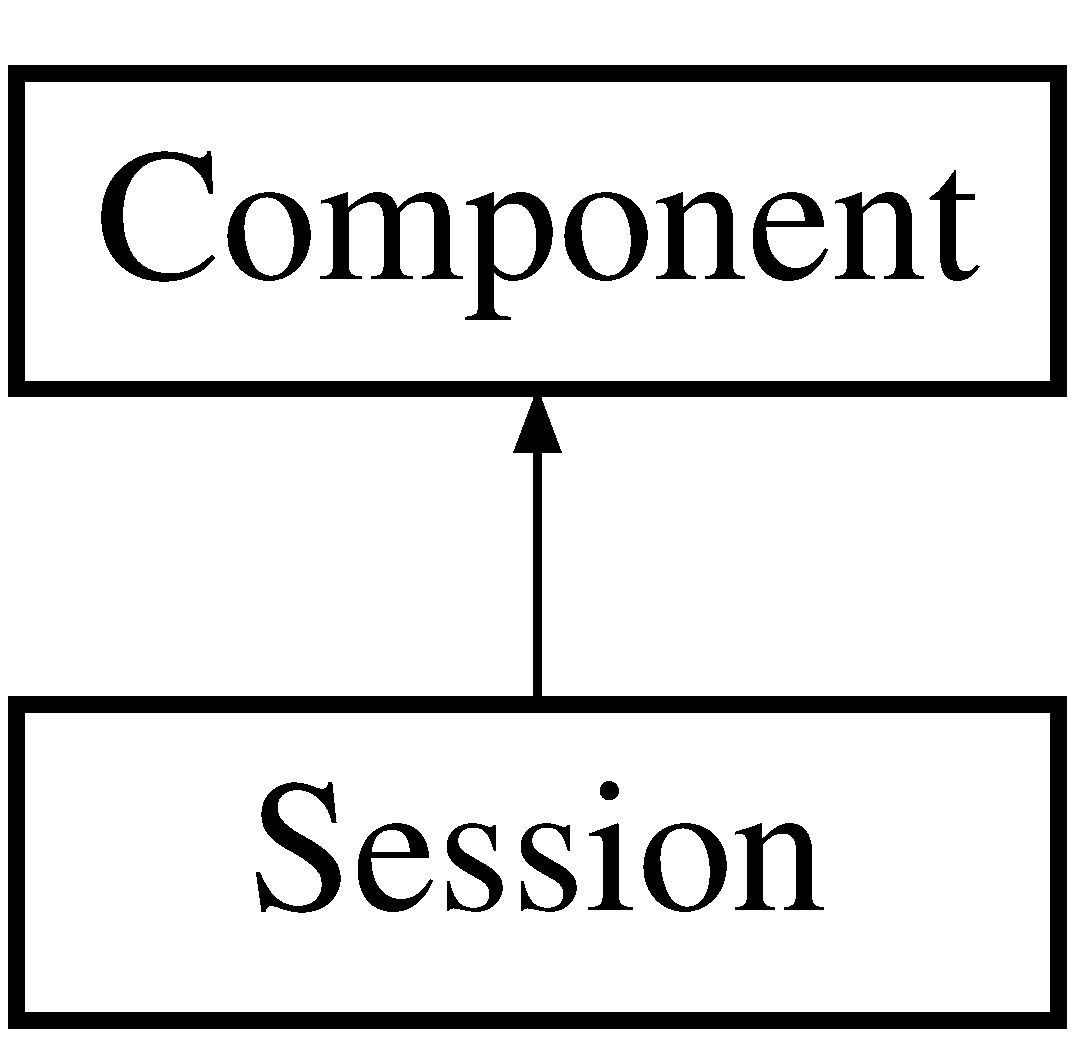
\includegraphics[height=2.000000cm]{classSession}
\end{center}
\end{figure}
\subsection*{Public Member Functions}
\begin{DoxyCompactItemize}
\item 
\hypertarget{classSession_a91bc789717d481ad5b4092fc7de9520c}{
{\bfseries start} ()}
\label{classSession_a91bc789717d481ad5b4092fc7de9520c}

\item 
\hypertarget{classSession_a71c2094d14dec32f7316332ce828ce9c}{
{\bfseries offsetSet} (\$offset, \$value)}
\label{classSession_a71c2094d14dec32f7316332ce828ce9c}

\item 
\hypertarget{classSession_add0611fb94dae2ef4f0c4ee42724a249}{
{\bfseries offsetGet} (\$offset)}
\label{classSession_add0611fb94dae2ef4f0c4ee42724a249}

\item 
\hypertarget{classSession_a984150b4571fcbe8501d3a980d49877a}{
{\bfseries offsetExists} (\$offset)}
\label{classSession_a984150b4571fcbe8501d3a980d49877a}

\item 
\hypertarget{classSession_a2f91fbb41ea4643fb6c83a64f2cfdc74}{
{\bfseries offsetUnset} (\$offset)}
\label{classSession_a2f91fbb41ea4643fb6c83a64f2cfdc74}

\item 
\hypertarget{classSession_a14e1fad994edf0ac73d617774c69dcfa}{
{\bfseries id} ()}
\label{classSession_a14e1fad994edf0ac73d617774c69dcfa}

\item 
\hypertarget{classSession_aaaeaf924cc8f951ae2adf7e182604b3f}{
{\bfseries destroy} ()}
\label{classSession_aaaeaf924cc8f951ae2adf7e182604b3f}

\item 
\hypertarget{classSession_a25b59d4868b28f083630a3d753c11f84}{
{\bfseries addFeedback} (\$message, \$status=0)}
\label{classSession_a25b59d4868b28f083630a3d753c11f84}

\item 
\hypertarget{classSession_ab71f5250f5f910d169ed61643d38fd2c}{
{\bfseries feedback} ()}
\label{classSession_ab71f5250f5f910d169ed61643d38fd2c}

\end{DoxyCompactItemize}
\subsection*{Public Attributes}
\begin{DoxyCompactItemize}
\item 
\hypertarget{classSession_a11be3c09c8b8328f776ab418bd918ba0}{
const {\bfseries cookieName} = '\hyperlink{classSession}{Session}'}
\label{classSession_a11be3c09c8b8328f776ab418bd918ba0}

\end{DoxyCompactItemize}
\subsection*{Protected Member Functions}
\begin{DoxyCompactItemize}
\item 
\hypertarget{classSession_a43eb64d79c4a35638f2d64265de4aa56}{
{\bfseries \_\-init} ()}
\label{classSession_a43eb64d79c4a35638f2d64265de4aa56}

\end{DoxyCompactItemize}
\subsection*{Protected Attributes}
\begin{DoxyCompactItemize}
\item 
\hypertarget{classSession_a4854a1f2ded7eb0c5e9c66f2830f92d6}{
{\bfseries \$\_\-id}}
\label{classSession_a4854a1f2ded7eb0c5e9c66f2830f92d6}

\end{DoxyCompactItemize}


The documentation for this class was generated from the following file:\begin{DoxyCompactItemize}
\item 
Component/Session.php\end{DoxyCompactItemize}

\hypertarget{classValidator}{
\section{Validator Class Reference}
\label{classValidator}\index{Validator@{Validator}}
}
\subsection*{Static Public Member Functions}
\begin{DoxyCompactItemize}
\item 
static \hyperlink{classValidator_a383fabe41373911648b022affce06392}{checkObject} (\$object, \$rules)
\item 
\hypertarget{classValidator_a7dff91acc69f50842aba95ae5ee25608}{
static {\bfseries checkMultiple} (\$values, \$rules, \$object=null)}
\label{classValidator_a7dff91acc69f50842aba95ae5ee25608}

\item 
static \hyperlink{classValidator_a7a1061f984896a168eed57d1d34fb433}{check} (\$value, \$rules, \$object=null)
\item 
\hypertarget{classValidator_aca327f59e0750df211529c61e54974b7}{
static {\bfseries validEmail} (\$value, \$params=array())}
\label{classValidator_aca327f59e0750df211529c61e54974b7}

\item 
\hypertarget{classValidator_abcfda5ed6af8a7338708b77c030aec55}{
static {\bfseries validInteger} (\$value, \$params=array())}
\label{classValidator_abcfda5ed6af8a7338708b77c030aec55}

\item 
\hypertarget{classValidator_ad7430c0c6f3e368ce9b3cb540564de2c}{
static {\bfseries validFloat} (\$value, \$params=array())}
\label{classValidator_ad7430c0c6f3e368ce9b3cb540564de2c}

\item 
\hypertarget{classValidator_ab0d9ddba42a629e59d6a562160b388a4}{
static {\bfseries validRequired} (\$value, \$params=array())}
\label{classValidator_ab0d9ddba42a629e59d6a562160b388a4}

\item 
\hypertarget{classValidator_a0b13d0bb343bf7a3e8b20e99506eac95}{
static {\bfseries validMaxLength} (\$value, \$params=array())}
\label{classValidator_a0b13d0bb343bf7a3e8b20e99506eac95}

\item 
\hypertarget{classValidator_aeacd793244066335aeda16fa1b398228}{
static {\bfseries validMinLength} (\$value, \$params=array())}
\label{classValidator_aeacd793244066335aeda16fa1b398228}

\end{DoxyCompactItemize}
\subsection*{Public Attributes}
\begin{DoxyCompactItemize}
\item 
\hypertarget{classValidator_a692588dd1512dbedfa8b50662191d7ca}{
const {\bfseries BLANK} = '/$^\wedge$$\backslash$s$\ast$\$/'}
\label{classValidator_a692588dd1512dbedfa8b50662191d7ca}

\item 
\hypertarget{classValidator_a9decf4aed87bde755cc40d7851d761cd}{
const {\bfseries VALID\_\-INTEGER} = '/$^\wedge$\mbox{[}-\/+\mbox{]}?$\backslash$d+\$/'}
\label{classValidator_a9decf4aed87bde755cc40d7851d761cd}

\item 
\hypertarget{classValidator_afd5191dafd4099abdd9be1db24173093}{
const {\bfseries VALID\_\-FLOAT} = '/$^\wedge$\mbox{[}-\/+\mbox{]}?$\backslash$d$\ast$$\backslash$.?$\backslash$d+\$/'}
\label{classValidator_afd5191dafd4099abdd9be1db24173093}

\item 
\hypertarget{classValidator_aaa6bc1384d036a033b57b74e9681f6ce}{
const {\bfseries VALID\_\-EMAIL} = '/$\backslash$b\mbox{[}A-\/Z0-\/9.\_\-\%+-\/\mbox{]}+@\mbox{[}A-\/Z0-\/9.-\/\mbox{]}+$\backslash$.\mbox{[}A-\/Z\mbox{]}\{2,4\}$\backslash$b/i'}
\label{classValidator_aaa6bc1384d036a033b57b74e9681f6ce}

\end{DoxyCompactItemize}


\subsection{Member Function Documentation}
\hypertarget{classValidator_a7a1061f984896a168eed57d1d34fb433}{
\index{Validator@{Validator}!check@{check}}
\index{check@{check}!Validator@{Validator}}
\subsubsection[{check}]{\setlength{\rightskip}{0pt plus 5cm}static Validator::check (
\begin{DoxyParamCaption}
\item[{\$}]{ value, }
\item[{\$}]{ rules, }
\item[{\$}]{ object = {\ttfamily null}}
\end{DoxyParamCaption}
)\hspace{0.3cm}{\ttfamily  \mbox{[}static\mbox{]}}}}
\label{classValidator_a7a1061f984896a168eed57d1d34fb433}
Checks a value, returns an array of errors 
\begin{DoxyParams}{Parameters}
\item[{\em mixed}]\$value \item[{\em array}]\$rules \item[{\em object}]\$object An object containing rule callbacks \end{DoxyParams}


Rules will not be checked if the value is blank and not required

\hypertarget{classValidator_a383fabe41373911648b022affce06392}{
\index{Validator@{Validator}!checkObject@{checkObject}}
\index{checkObject@{checkObject}!Validator@{Validator}}
\subsubsection[{checkObject}]{\setlength{\rightskip}{0pt plus 5cm}static Validator::checkObject (
\begin{DoxyParamCaption}
\item[{\$}]{ object, }
\item[{\$}]{ rules}
\end{DoxyParamCaption}
)\hspace{0.3cm}{\ttfamily  \mbox{[}static\mbox{]}}}}
\label{classValidator_a383fabe41373911648b022affce06392}
Validates an object, returning an array of errors 

The documentation for this class was generated from the following file:\begin{DoxyCompactItemize}
\item 
libs/Library/Validator.php\end{DoxyCompactItemize}

\hypertarget{classView}{
\section{View Class Reference}
\label{classView}\index{View@{View}}
}
\subsection*{Public Member Functions}
\begin{DoxyCompactItemize}
\item 
\hypertarget{classView_aff2c8a304801730574b5bc109c482e09}{
{\bfseries \_\-\_\-construct} (\$response)}
\label{classView_aff2c8a304801730574b5bc109c482e09}

\item 
\hyperlink{classView_a82676edf021e4e4e89bd6d4876ad7fb9}{\_\-\_\-get} (\$name)
\item 
\hypertarget{classView_a1dab1e88315e34d6f4c74b75ca12f12d}{
{\bfseries render} (\$data)}
\label{classView_a1dab1e88315e34d6f4c74b75ca12f12d}

\item 
\hypertarget{classView_ad28ba2a16ab546f22dd5a60e65f20d2a}{
{\bfseries partial} (\$partial, \$data=array())}
\label{classView_ad28ba2a16ab546f22dd5a60e65f20d2a}

\item 
\hypertarget{classView_a1e38f96f791a0d264ea794ccd1c7c8ee}{
{\bfseries isAjax} ()}
\label{classView_a1e38f96f791a0d264ea794ccd1c7c8ee}

\item 
\hypertarget{classView_ab4e4860b85376521eff6579b1f386715}{
{\bfseries path} (\$route=null)}
\label{classView_ab4e4860b85376521eff6579b1f386715}

\item 
\hypertarget{classView_a604713b6fdc5d37523d60839652fdcd5}{
{\bfseries webroot} (\$resource= '')}
\label{classView_a604713b6fdc5d37523d60839652fdcd5}

\item 
\hypertarget{classView_acb1fea2da6c574abd3954f1c9271d451}{
{\bfseries modGet} (\$changes=array())}
\label{classView_acb1fea2da6c574abd3954f1c9271d451}

\item 
\hypertarget{classView_a3c6dd7873c2b0bb4e4d9e39638c42bb0}{
{\bfseries ajax} (\$route, \$data=array(), \$method= 'GET')}
\label{classView_a3c6dd7873c2b0bb4e4d9e39638c42bb0}

\item 
\hypertarget{classView_a91dbfe549a40feaacb321d64997461fa}{
{\bfseries layout} (\$layout=null)}
\label{classView_a91dbfe549a40feaacb321d64997461fa}

\end{DoxyCompactItemize}
\subsection*{Protected Member Functions}
\begin{DoxyCompactItemize}
\item 
\hyperlink{classView_afd382c9e42d6c24b8a064b615db7a898}{\_\-renderContent} (\$data)
\item 
\hyperlink{classView_a2cc8578430d33232105f4bab57978e7c}{\_\-findTemplate} ()
\item 
\hyperlink{classView_a0ff5857aa83ff98b3eb7e6067469cd54}{\_\-templatePath} (\$file)
\item 
\hypertarget{classView_ab0a86a216c1ad07e4580a4574f9b32e9}{
{\bfseries \_\-renderFile} (\$\_\-\_\-\_\-file, \$\_\-\_\-\_\-data)}
\label{classView_ab0a86a216c1ad07e4580a4574f9b32e9}

\item 
\hypertarget{classView_abe4a1f48ac5a9a9ebfd7a9292a8db663}{
{\bfseries \_\-helper} (\$name)}
\label{classView_abe4a1f48ac5a9a9ebfd7a9292a8db663}

\end{DoxyCompactItemize}
\subsection*{Protected Attributes}
\begin{DoxyCompactItemize}
\item 
\hypertarget{classView_a9896fc61a6f4aebec58668abf395db23}{
{\bfseries \$\_\-helpers}}
\label{classView_a9896fc61a6f4aebec58668abf395db23}

\item 
\hypertarget{classView_ad18c95369471c2fb61d0741b8d4040de}{
{\bfseries \$\_\-Response}}
\label{classView_ad18c95369471c2fb61d0741b8d4040de}

\item 
\hypertarget{classView_afdee45797fa2902521e300d19383cec8}{
{\bfseries \$\_\-layoutData} = array()}
\label{classView_afdee45797fa2902521e300d19383cec8}

\item 
\hypertarget{classView_a78921c86c8bc1798465462b9f0704e09}{
{\bfseries \$\_\-layout} = 'default'}
\label{classView_a78921c86c8bc1798465462b9f0704e09}

\item 
\hypertarget{classView_aa46abe6eae0fa132506c23fa782c1d5e}{
{\bfseries \$\_\-templateDir}}
\label{classView_aa46abe6eae0fa132506c23fa782c1d5e}

\end{DoxyCompactItemize}


\subsection{Member Function Documentation}
\hypertarget{classView_a82676edf021e4e4e89bd6d4876ad7fb9}{
\index{View@{View}!\_\-\_\-get@{\_\-\_\-get}}
\index{\_\-\_\-get@{\_\-\_\-get}!View@{View}}
\subsubsection[{\_\-\_\-get}]{\setlength{\rightskip}{0pt plus 5cm}View::\_\-\_\-get (
\begin{DoxyParamCaption}
\item[{\$}]{ name}
\end{DoxyParamCaption}
)}}
\label{classView_a82676edf021e4e4e89bd6d4876ad7fb9}
Attempt to load Helpers on-\/demand \hypertarget{classView_a2cc8578430d33232105f4bab57978e7c}{
\index{View@{View}!\_\-findTemplate@{\_\-findTemplate}}
\index{\_\-findTemplate@{\_\-findTemplate}!View@{View}}
\subsubsection[{\_\-findTemplate}]{\setlength{\rightskip}{0pt plus 5cm}View::\_\-findTemplate (
\begin{DoxyParamCaption}
{}
\end{DoxyParamCaption}
)\hspace{0.3cm}{\ttfamily  \mbox{[}protected\mbox{]}}}}
\label{classView_a2cc8578430d33232105f4bab57978e7c}
Attempts to find the template file for rendering. This is based on the request route and the response status. \begin{DoxyReturn}{Returns}
string The path to the template, relative to the views direcetory 
\end{DoxyReturn}
\hypertarget{classView_afd382c9e42d6c24b8a064b615db7a898}{
\index{View@{View}!\_\-renderContent@{\_\-renderContent}}
\index{\_\-renderContent@{\_\-renderContent}!View@{View}}
\subsubsection[{\_\-renderContent}]{\setlength{\rightskip}{0pt plus 5cm}View::\_\-renderContent (
\begin{DoxyParamCaption}
\item[{\$}]{ data}
\end{DoxyParamCaption}
)\hspace{0.3cm}{\ttfamily  \mbox{[}protected\mbox{]}}}}
\label{classView_afd382c9e42d6c24b8a064b615db7a898}
Renders the content template with the data supplied from the controller. If the template file does not exist, the response will be sent as JSON, without a layout. \begin{DoxyReturn}{Returns}
string 
\end{DoxyReturn}
\hypertarget{classView_a0ff5857aa83ff98b3eb7e6067469cd54}{
\index{View@{View}!\_\-templatePath@{\_\-templatePath}}
\index{\_\-templatePath@{\_\-templatePath}!View@{View}}
\subsubsection[{\_\-templatePath}]{\setlength{\rightskip}{0pt plus 5cm}View::\_\-templatePath (
\begin{DoxyParamCaption}
\item[{\$}]{ file}
\end{DoxyParamCaption}
)\hspace{0.3cm}{\ttfamily  \mbox{[}protected\mbox{]}}}}
\label{classView_a0ff5857aa83ff98b3eb7e6067469cd54}
Returns the absolute path to the specified template file. 
\begin{DoxyParams}{Parameters}
\item[{\em string}]\$file \end{DoxyParams}
\begin{DoxyReturn}{Returns}
string the absolute path to the file, or null if it does not exist 
\end{DoxyReturn}


The documentation for this class was generated from the following file:\begin{DoxyCompactItemize}
\item 
libs/View.php\end{DoxyCompactItemize}

\hypertarget{classXRequest}{
\section{XRequest Class Reference}
\label{classXRequest}\index{XRequest@{XRequest}}
}
\subsection*{Public Member Functions}
\begin{DoxyCompactItemize}
\item 
\hyperlink{classXRequest_abf5cb6cee4e104ed2a6fa9cc1659fe79}{\_\-\_\-construct} (\$uri, \$data=array(), \$method= 'GET', \$headers=array())
\item 
\hyperlink{classXRequest_a7cc9ccf8e01f3fd885029d0a04281c75}{\_\-\_\-get} (\$name)
\item 
\hyperlink{classXRequest_afff17e6f3ff03dfb594f801992074389}{execute} ()
\item 
\hyperlink{classXRequest_a0c1a9397c901f52e2cc0f79d6d3aa76b}{handle} ()
\end{DoxyCompactItemize}
\subsection*{Protected Attributes}
\begin{DoxyCompactItemize}
\item 
\hypertarget{classXRequest_a24be959a56bd280ffa08b4a7e3676d88}{
{\bfseries \$\_\-handle}}
\label{classXRequest_a24be959a56bd280ffa08b4a7e3676d88}

\item 
\hypertarget{classXRequest_a5aca604d767ee86e5c66f6b15f71ace9}{
{\bfseries \$\_\-data}}
\label{classXRequest_a5aca604d767ee86e5c66f6b15f71ace9}

\item 
\hypertarget{classXRequest_a549e72fc8aa404e33c671d0bda3bd4e1}{
{\bfseries \$\_\-headers}}
\label{classXRequest_a549e72fc8aa404e33c671d0bda3bd4e1}

\item 
\hypertarget{classXRequest_af1c7a52b0b4b8a1a8d3dd91951cc9020}{
{\bfseries \$\_\-method}}
\label{classXRequest_af1c7a52b0b4b8a1a8d3dd91951cc9020}

\item 
\hypertarget{classXRequest_a936fb5c46a0975b29428a7b1df3d05a5}{
{\bfseries \$\_\-Response}}
\label{classXRequest_a936fb5c46a0975b29428a7b1df3d05a5}

\end{DoxyCompactItemize}


\subsection{Detailed Description}
External \hyperlink{classRequest}{Request} class

This class immitates behaviours of the standard \hyperlink{classRequest}{Request} class, but applies to external requests to sources outside of the current application. 

\subsection{Constructor \& Destructor Documentation}
\hypertarget{classXRequest_abf5cb6cee4e104ed2a6fa9cc1659fe79}{
\index{XRequest@{XRequest}!\_\-\_\-construct@{\_\-\_\-construct}}
\index{\_\-\_\-construct@{\_\-\_\-construct}!XRequest@{XRequest}}
\subsubsection[{\_\-\_\-construct}]{\setlength{\rightskip}{0pt plus 5cm}XRequest::\_\-\_\-construct (
\begin{DoxyParamCaption}
\item[{\$}]{ uri, }
\item[{\$}]{ data = {\ttfamily array()}, }
\item[{\$}]{ method = {\ttfamily 'GET'}, }
\item[{\$}]{ headers = {\ttfamily array()}}
\end{DoxyParamCaption}
)}}
\label{classXRequest_abf5cb6cee4e104ed2a6fa9cc1659fe79}
Constructor. 
\begin{DoxyParams}{Parameters}
\item[{\em string}]\$uri The URI to which the request is made \item[{\em array}]\$data The data to send in the request \item[{\em string}]\$method The request method \item[{\em array}]\$headers \hyperlink{classRequest}{Request} headers \end{DoxyParams}


\subsection{Member Function Documentation}
\hypertarget{classXRequest_a7cc9ccf8e01f3fd885029d0a04281c75}{
\index{XRequest@{XRequest}!\_\-\_\-get@{\_\-\_\-get}}
\index{\_\-\_\-get@{\_\-\_\-get}!XRequest@{XRequest}}
\subsubsection[{\_\-\_\-get}]{\setlength{\rightskip}{0pt plus 5cm}XRequest::\_\-\_\-get (
\begin{DoxyParamCaption}
\item[{\$}]{ name}
\end{DoxyParamCaption}
)}}
\label{classXRequest_a7cc9ccf8e01f3fd885029d0a04281c75}
Immitate read-\/only properties 
\begin{DoxyParams}{Parameters}
\item[{\em string}]\$name \end{DoxyParams}
\begin{DoxyReturn}{Returns}
mixed 
\end{DoxyReturn}
\hypertarget{classXRequest_afff17e6f3ff03dfb594f801992074389}{
\index{XRequest@{XRequest}!execute@{execute}}
\index{execute@{execute}!XRequest@{XRequest}}
\subsubsection[{execute}]{\setlength{\rightskip}{0pt plus 5cm}XRequest::execute (
\begin{DoxyParamCaption}
{}
\end{DoxyParamCaption}
)}}
\label{classXRequest_afff17e6f3ff03dfb594f801992074389}
Executes the request. \begin{DoxyReturn}{Returns}
mixed False if the request fails, or a \hyperlink{classFrawst}{Frawst} object if it's successful. 
\end{DoxyReturn}
\hypertarget{classXRequest_a0c1a9397c901f52e2cc0f79d6d3aa76b}{
\index{XRequest@{XRequest}!handle@{handle}}
\index{handle@{handle}!XRequest@{XRequest}}
\subsubsection[{handle}]{\setlength{\rightskip}{0pt plus 5cm}resource The cURL XRequest::handle (
\begin{DoxyParamCaption}
{}
\end{DoxyParamCaption}
)}}
\label{classXRequest_a0c1a9397c901f52e2cc0f79d6d3aa76b}
Returns the curl file handle used for this request. Only available after \hyperlink{classXRequest_afff17e6f3ff03dfb594f801992074389}{execute()} is invoked. \begin{DoxyReturn}{Returns}
resource 
\end{DoxyReturn}


The documentation for this class was generated from the following file:\begin{DoxyCompactItemize}
\item 
XRequest.php\end{DoxyCompactItemize}

\hypertarget{classXResponse}{
\section{XResponse Class Reference}
\label{classXResponse}\index{XResponse@{XResponse}}
}
\subsection*{Public Member Functions}
\begin{DoxyCompactItemize}
\item 
\hyperlink{classXResponse_af849678ed30158fdafa5262268ac574b}{\_\-\_\-construct} (\$request)
\item 
\hyperlink{classXResponse_a24a0d2be8802d014c8d658f27acbabf3}{\_\-\_\-get} (\$name)
\item 
\hyperlink{classXResponse_a54fe154d0117afb0ab6a5b78e71ea40e}{pullInfo} (\$data)
\item 
\hyperlink{classXResponse_a9cff5d76bbba302e8c71c8d115acc95f}{data} ()
\item 
\hyperlink{classXResponse_a2217ce89a8e77e82af4ffbe824f247f5}{headers} ()
\item 
\hyperlink{classXResponse_af5f8f0b906cc013e23d021796c3b6a74}{header} (\$name)
\item 
\hyperlink{classXResponse_a9d07b3800d366327e85977b602260959}{contentType} (\$encoding=false)
\end{DoxyCompactItemize}
\subsection*{Protected Attributes}
\begin{DoxyCompactItemize}
\item 
\hypertarget{classXResponse_af50c9aade6da0fd92bed4703f8c0de08}{
{\bfseries \$\_\-Request}}
\label{classXResponse_af50c9aade6da0fd92bed4703f8c0de08}

\item 
\hypertarget{classXResponse_a91083c41b254ad9423a56d025490c360}{
{\bfseries \$\_\-data}}
\label{classXResponse_a91083c41b254ad9423a56d025490c360}

\item 
\hypertarget{classXResponse_af76024af526545dfcd82b7c2ad3709ac}{
{\bfseries \$\_\-headers} = array()}
\label{classXResponse_af76024af526545dfcd82b7c2ad3709ac}

\end{DoxyCompactItemize}


\subsection{Detailed Description}
Handles response to external requests. 

\subsection{Constructor \& Destructor Documentation}
\hypertarget{classXResponse_af849678ed30158fdafa5262268ac574b}{
\index{XResponse@{XResponse}!\_\-\_\-construct@{\_\-\_\-construct}}
\index{\_\-\_\-construct@{\_\-\_\-construct}!XResponse@{XResponse}}
\subsubsection[{\_\-\_\-construct}]{\setlength{\rightskip}{0pt plus 5cm}XResponse::\_\-\_\-construct (
\begin{DoxyParamCaption}
\item[{\$}]{ request}
\end{DoxyParamCaption}
)}}
\label{classXResponse_af849678ed30158fdafa5262268ac574b}
Constructor. 
\begin{DoxyParams}{Parameters}
\item[{\em Frawst$\backslash$XRequest}]\hyperlink{classRequest}{Request} that is being responded to \end{DoxyParams}


\subsection{Member Function Documentation}
\hypertarget{classXResponse_a24a0d2be8802d014c8d658f27acbabf3}{
\index{XResponse@{XResponse}!\_\-\_\-get@{\_\-\_\-get}}
\index{\_\-\_\-get@{\_\-\_\-get}!XResponse@{XResponse}}
\subsubsection[{\_\-\_\-get}]{\setlength{\rightskip}{0pt plus 5cm}XResponse::\_\-\_\-get (
\begin{DoxyParamCaption}
\item[{\$}]{ name}
\end{DoxyParamCaption}
)}}
\label{classXResponse_a24a0d2be8802d014c8d658f27acbabf3}
Read-\/only immitation. 
\begin{DoxyParams}{Parameters}
\item[{\em string}]\$name \end{DoxyParams}
\begin{DoxyReturn}{Returns}
mixed 
\end{DoxyReturn}
\hypertarget{classXResponse_a9d07b3800d366327e85977b602260959}{
\index{XResponse@{XResponse}!contentType@{contentType}}
\index{contentType@{contentType}!XResponse@{XResponse}}
\subsubsection[{contentType}]{\setlength{\rightskip}{0pt plus 5cm}XResponse::contentType (
\begin{DoxyParamCaption}
\item[{\$}]{ encoding = {\ttfamily false}}
\end{DoxyParamCaption}
)}}
\label{classXResponse_a9d07b3800d366327e85977b602260959}
Convenience method for getting the response Content-\/Type. 
\begin{DoxyParams}{Parameters}
\item[{\em bool}]\$encoding If false, the content encoding will not be returned \end{DoxyParams}
\begin{DoxyReturn}{Returns}
string The response Content-\/Type 
\end{DoxyReturn}
\hypertarget{classXResponse_a9cff5d76bbba302e8c71c8d115acc95f}{
\index{XResponse@{XResponse}!data@{data}}
\index{data@{data}!XResponse@{XResponse}}
\subsubsection[{data}]{\setlength{\rightskip}{0pt plus 5cm}array {\bf Response} XResponse::data (
\begin{DoxyParamCaption}
{}
\end{DoxyParamCaption}
)}}
\label{classXResponse_a9cff5d76bbba302e8c71c8d115acc95f}
Returns the response data. \begin{DoxyReturn}{Returns}
mixed \hyperlink{classResponse}{Response} data 
\end{DoxyReturn}
\hypertarget{classXResponse_af5f8f0b906cc013e23d021796c3b6a74}{
\index{XResponse@{XResponse}!header@{header}}
\index{header@{header}!XResponse@{XResponse}}
\subsubsection[{header}]{\setlength{\rightskip}{0pt plus 5cm}XResponse::header (
\begin{DoxyParamCaption}
\item[{\$}]{ name}
\end{DoxyParamCaption}
)}}
\label{classXResponse_af5f8f0b906cc013e23d021796c3b6a74}
Returns the value of a response header. 
\begin{DoxyParams}{Parameters}
\item[{\em string}]\$name The name of the header \end{DoxyParams}
\begin{DoxyReturn}{Returns}
string The response header value or null if not set 
\end{DoxyReturn}
\hypertarget{classXResponse_a2217ce89a8e77e82af4ffbe824f247f5}{
\index{XResponse@{XResponse}!headers@{headers}}
\index{headers@{headers}!XResponse@{XResponse}}
\subsubsection[{headers}]{\setlength{\rightskip}{0pt plus 5cm}XResponse::headers (
\begin{DoxyParamCaption}
{}
\end{DoxyParamCaption}
)}}
\label{classXResponse_a2217ce89a8e77e82af4ffbe824f247f5}
\begin{DoxyReturn}{Returns}
array Associative array of response headers 
\end{DoxyReturn}
\hypertarget{classXResponse_a54fe154d0117afb0ab6a5b78e71ea40e}{
\index{XResponse@{XResponse}!pullInfo@{pullInfo}}
\index{pullInfo@{pullInfo}!XResponse@{XResponse}}
\subsubsection[{pullInfo}]{\setlength{\rightskip}{0pt plus 5cm}XResponse::pullInfo (
\begin{DoxyParamCaption}
\item[{\$}]{ data}
\end{DoxyParamCaption}
)}}
\label{classXResponse_a54fe154d0117afb0ab6a5b78e71ea40e}
Pulls response info from the \hyperlink{classRequest}{Request}. 

The documentation for this class was generated from the following file:\begin{DoxyCompactItemize}
\item 
libs/XResponse.php\end{DoxyCompactItemize}

\chapter{Example Documentation}
\hypertarget{form-example}{
\section{form}
}
Associative array of data sent to this request data from a POST request, querystring data from GET


\begin{DoxyCodeInclude}
\end{DoxyCodeInclude}
 
\hypertarget{POST-example}{
\section{POST}
}
The method through which this request was performed '


\begin{DoxyCodeInclude}
\end{DoxyCodeInclude}
 
\printindex
\end{document}
